\documentclass[twoside]{article}

%\usepackage{aistats2022}
% If your paper is accepted, change the options for the package
% aistats2022 as follows:
%
\usepackage[accepted]{aistats2022}
\usepackage{wrapfig}
\usepackage[dvipsnames]{xcolor}
\usepackage{adjustbox}
\usepackage{tcolorbox}
\usepackage{rotating}
\usepackage{dblfloatfix}
\usepackage{xparse}
\usepackage{mathtools}
\usepackage{centernot}
\usepackage{epsfig}
\usepackage{graphicx}
\usepackage{amssymb,amsmath}%showkeys}
\usepackage{enumerate}
\usepackage{verbatim}
%\usepackage{multirow}
\usepackage{multicol}
\usepackage[english]{babel}
\usepackage{color}
\usepackage{float}
\usepackage{hyperref}
\usepackage{tabularx}
\hypersetup{
     colorlinks=true,
     linkcolor=blue,
     citecolor=blue,
     filecolor=blue,
     urlcolor=blue,
}
\usepackage{setspace}
\usepackage{mathrsfs}
\usepackage{multirow}
\usepackage{stackengine}
\usepackage[skip=0pt]{caption}
%\usepackage{rotating}
%\usepackage{pdflscape}
\setlength{\oddsidemargin}{-0.125in} \setlength{\topmargin}{-0.5in}
\setlength{\textwidth}{6.5in} \setlength{\textheight}{9in}
\setlength{\textheight}{9in} \setlength{\textwidth}{6.5in}
\setlength{\topmargin}{-36pt} \setlength{\oddsidemargin}{0pt}
\setlength{\evensidemargin}{0pt} \tolerance=500

%%%%%%%%%%%%%%%%%%%%%%%%%%%%%%%%%%%%%%%%%%
\def\rayL{X}
\def\raybeta{{\cal B}}
\def\rayalpha{\alpha}
\def\raymatern{{\cal M}}

\def\tvacomment#1{\vskip 2mm\boxit{\vskip 2mm{\color{blue}\bf \bf#1} {\color{magenta}\bf \bf -- TVA\vskip 2mm}}\vskip 2mm}
\def\mggcomment#1{\vskip 2mm\boxit{\vskip 2mm{\color{magenta}\bf \bf#1} {\color{black}\bf -- MGG\vskip 2mm}}\vskip 2mm}
%%%%%%%%%%%%%%%%%%%%%%%%%%%%%%%%%%%%%%%%%%

%%%%%%%%%%%%%%%%%%%%%%%%%%%%%%%%%%%%%%%%%%
\def\wt{\widetilde}
\def\diag{\hbox{diag}}
\def\wh{\widehat}
\def\AIC{\hbox{AIC}}
\def\BIC{\hbox{BIC}}
%- Makes the section title start with Appendix in the appendix environment
\newcommand{\Appendix}
{%\appendix
\def\thesection{Appendix~\Alph{section}}
%\def\thesubsection{\Alph{section}.\arabic{subsection}}
\def\thesubsection{A.\arabic{subsection}}
}
\def\diag{\hbox{diag}}
\def\log{\hbox{log}}
\def\bias{\hbox{bias}}
\def\Siuu{\boldSigma_{i,uu}}
\def\dfrac#1#2{{\displaystyle{#1\over#2}}}
\def\VS{{\vskip 3mm\noindent}}
\def\boxit#1{\vbox{\hrule\hbox{\vrule\kern6pt
          \vbox{\kern6pt#1\kern6pt}\kern6pt\vrule}\hrule}}
\def\refhg{\hangindent=20pt\hangafter=1}
\def\refmark{\par\vskip 2mm\noindent\refhg}
\def\naive{\hbox{naive}}
\def\itemitem{\par\indent \hangindent2\parindent \textindent}
\def\var{\hbox{var}}
\def\Corr{\hbox{Corr}}
\def\Corr{\hbox{Corr}}
\def\trace{\hbox{trace}}
\def\refhg{\hangindent=20pt\hangafter=1}
\def\refmark{\par\vskip 2mm\noindent\refhg}
\def\Normal{\hbox{Normal}}
\def\povr{\buildrel p\over\to}
\def\ccdot{{\bullet}}
\def\bse{\begin{eqnarray*}}
\def\ese{\end{eqnarray*}}
\def\be{\begin{eqnarray}}
\def\ee{\end{eqnarray}}
\def\bq{\begin{equation}}
\def\eq{\end{equation}}
\def\bse{\begin{eqnarray*}}
\def\ese{\end{eqnarray*}}
\def\pr{\hbox{pr}}
\def\wh{\widehat}
\def\trans{^{\rm T}}
\def\myalpha{{\cal A}}
\def\th{^{th}}

\newcommand{\bbR}{\mathbb{R}}
\newcommand{\bbX}{\mathbb{X}}
\newcommand{\bI}{\mathbf{I}}
\newcommand{\bM}{\mathbf{M}}
\newcommand{\bX}{\mathbf{X}}
\newcommand{\bY}{\mathbf{Y}}
\newcommand{\bZ}{\mathbf{Z}}
\newcommand{\bA}{\mathbf{A}}
\newcommand{\bB}{\mathbf{B}}
\newcommand{\bC}{\mathbf{C}}
\newcommand{\bD}{\mathbf{D}}
\newcommand{\bF}{\mathbf{F}}
\newcommand{\bG}{\mathbf{G}}
\newcommand{\bP}{\mathbf{P}}
\newcommand{\bR}{\mathbf{R}}
\newcommand{\bS}{\mathbf{S}}
\newcommand{\bU}{\mathbf{U}}
\newcommand{\bV}{\mathbf{V}}
\newcommand{\br}{\mathbf{r}}
\newcommand{\bL}{\mathbf{L}}
\newcommand{\bW}{\mathbf{W}}
\newcommand{\bT}{\mathbf{T}}
\newcommand{\bH}{\mathbf{H}}
\newcommand{\bx}{\mathbf{x}}
\newcommand{\bz}{\mathbf{z}}
\newcommand{\bs}{\mathbf{s}}
\newcommand{\bu}{\mathbf{u}}
\newcommand{\ba}{\mathbf{a}}
\newcommand{\bb}{\mathbf{b}}
\newcommand{\by}{\mathbf{y}}
\newcommand{\bc}{\mathbf{c}}
\newcommand{\bv}{\mathbf{v}}
\newcommand{\bm}{\mathbf{m}}
\newcommand{\bw}{\mathbf{w}}
\newcommand{\bd}{\mathbf{d}}
\newcommand{\bt}{\mathbf{t}}
%\newcommand{\be}{\mathbf{\mathcal{E}}}
\newcommand{\bmu}{\boldsymbol{\mu}}
\newcommand{\bdelta}{\boldsymbol{\delta}}
\newcommand{\bepsilon}{\boldsymbol{\epsilon}}
\newcommand{\balpha}{\boldsymbol{\alpha}}
\newcommand{\bbeta}{\boldsymbol{\beta}}
\newcommand{\bnu}{\boldsymbol{\nu}}
%\newcommand{\btheta}{\boldsymbol{\theta}}
\newcommand{\bLambda}{\boldsymbol{\psi}}
\newcommand{\bSigma}{\boldsymbol{\Sigma}}
\newcommand{\bGamma}{\boldsymbol{\Gamma}}
\newcommand{\bOmega}{\boldsymbol{\Omega}}
\newcommand{\bDelta}{\boldsymbol{\Delta}}
\newcommand{\bgamma}{\boldsymbol{\gamma}}
\newcommand{\blambda}{\boldsymbol{\lambda}}
\newcommand{\bxi}{\boldsymbol{\xi}}
\newcommand{\bomega}{\boldsymbol{\omega}}
\newcommand{\0}{\mathbf{0}}
\newcommand{\1}{\mathbf{1}}
\newcommand*{\QEDB}{\hfill\ensuremath{\square}}
\DeclareRobustCommand{\rchi}{{\mathpalette\irchi\relax}}
\newcommand{\irchi}[2]{\raisebox{\depth}{$#1\chi$}} % inner command, used by \rchi
%\newcommand{\rchi}{\mathscr X}
\newcommand{\argmin}{\operatornamewithlimits{arg\,min}}
\newcommand{\argmax}{\operatornamewithlimits{arg\,max}}
%###################################

\numberwithin{equation}{section}
\newtheorem{thm}{Theorem}[section]
\newtheorem{cor}[thm]{Corollary}
\newtheorem{lem}[thm]{Lemma}
\newtheorem{lemma}[thm]{Lemma}
\newtheorem{ex}{Example}
\newcommand{\bl}{\color{blue}}

\allowdisplaybreaks
\title{On some robust classifiers for high-dimensional data}%, low sample size
% If you set papersize explicitly, activate the following three lines:
\special{papersize = 8.5in, 11in}
\setlength{\pdfpageheight}{11in}
\setlength{\pdfpagewidth}{8.5in}

% If you use natbib package, activate the following three lines:
\usepackage[round]{natbib}
\renewcommand{\bibname}{References}
\renewcommand{\bibsection}{\subsubsection*{\bibname}}

% If you use BibTeX in apalike style, activate the following line:
\bibliographystyle{apalike}

\begin{document}

% If your paper is accepted and the title of your paper is very long,
% the style will print as headings an error message. Use the following
% command to supply a shorter title of your paper so that it can be
% used as headings.
%
%\runningtitle{I use this title instead because the last one was very long}

% If your paper is accepted and the number of authors is large, the
% style will print as headings an error message. Use the following
% command to supply a shorter version of the authors names so that
% they can be used as headings (for example, use only the surnames)
%
%\runningauthor{Surname 1, Surname 2, Surname 3, ...., Surname n}

\twocolumn[

\aistatstitle{On Some Fast And Robust Classifiers For High Dimension, Low Sample Size Data}

\aistatsauthor{Sarbojit Roy \And Jyotishka Ray Choudhury \And Subhajit Dutta }

\aistatsaddress{ {\it Indian Institute of Technology}\\ {\it Kanpur, India}\\ {\it sarbojit@iitk.ac.in} \And {\it Indian Statistical Institute}\\ {\it Kolkata, India}\\ {\it bs1903@isical.ac.in} \And  {\it Indian Institute of Technology}\\ {\it Kanpur, India} \\ {\it duttas@iitk.ac.in}}]

\begin{abstract}
In high dimension, low sample size (HDLSS) settings, \emph{distance concentration} phenomena affects the performance of several popular classifiers which are based on Euclidean distances. The behaviour of these classifiers in high dimensions is completely governed by the first and second order moments of the underlying class distributions. Moreover, the classifiers become useless for such HDLSS data when the first two moments of the competing distributions are equal, or when the moments do not exist. In this work, we propose robust, computationally efficient and tuning-free classifiers applicable in the HDLSS scenario. As the data dimension increases, these classifiers yield \emph{perfect classification} if the one-dimensional marginals of the underlying distributions are different. We establish strong theoretical properties for the proposed classifiers in \emph{ultrahigh-dimensional} settings. Numerical experiments with a wide variety of simulated examples and analysis of real data sets exhibit clear and convincing advantages over existing methods.
\end{abstract}

\section{INTRODUCTION}\label{intro}
Let us consider a classification problem involving two distribution functions $\bF_1$ and $\bF_2$ on $\mathbb{R}^p$ with $p\geq 1$. Suppose $\bX_i=(X_{i1},\ldots, X_{ip})^\top$ and $\bY_j=(Y_{j1},\ldots, Y_{jp})^\top$ are independent and identically distributed (i.i.d.) random vectors following $\bF_1$ and $\bF_2,$ respectively, for $1\le i\le n_1$ and $ 1\le j\le n_2.$ Let $\rchi = \rchi_1\cup \rchi_2$ be the training sample of size $n=n_1+n_2$, where $\rchi_1=\{\bX_{1},\ldots,\bX_{n_1}\}$ and
$\rchi_2=\{\bY_{1},\ldots,\bY_{n_2}\}$. We develop classifiers that yield {\it perfect classification} under fairly general conditions in high dimension, low sample size (HDLSS) settings, where the sample size $n$ remains fixed, but the dimension $p$ increases. A classifier $\delta$ is said to yield {\it perfect classification} in the HDLSS setting if the misclassification probability of $\delta$ goes to 0 as $p\to\infty.$
\begin{tcolorbox}[colback=white]
% \begin{itemize}
% \setlength{\itemindent}{-2em}
\noindent In the classical setting, $p$ is fixed and $n\to\infty$. Information is accumulated as more samples are collected.\newline

\noindent In HDLSS settings, $n$ is fixed while $p\to\infty$. Information is accumulated as  more features are measured.
% \end{itemize}
\end{tcolorbox}
\subsection{Literature Review}
In the HDLSS asymptotic regime, Euclidean distance (ED) based classifiers face some natural drawbacks due to \emph{distance concentration} \citep{aggarwal2001surprising,francois2007concentration}. To give a mathematical exposition of this fact, let $\bmu_j$ and $\Sigma_j$ denote the mean vector and the covariance matrix of $\bF_j$ for $j=1,2$. We assume that the following limits exist:
\vspace{-0.15cm}
\begin{align}\label{limconst1}
\small
%  &\nu_{11} = \frac{1}{p}\lim\limits_{p\to\infty}\bmu_1^\top\bmu_1,\ \nu_{12} = \frac{1}{p}\lim\limits_{p\to\infty}\bmu_1^\top\bmu_2,\nonumber \\
%  &\nu_{22} = \frac{1}{p}\lim\limits_{p\to\infty}\bmu_2^\top\bmu_2,
& \nu^2 = \lim\limits_{p\to\infty}\frac{1}{p}\|\bmu_1-\bmu_2\|^2\text{ and }\nonumber\\
& \sigma_j^2 = \lim\limits_{p\to\infty}\frac{1}{p} tr  (\Sigma_j)\text{ for }  j= 1,2.
%   \sigma_2^2 = \frac{1}{p}\lim\limits_{p\to\infty} tr (\Sigma_2).
\end{align}
Here, $\|\cdot\|$ denotes the Euclidean norm on $\mathbb{R}^p$ and $tr (M)$ denotes the trace of a $p\times p$ matrix $M$. The constants $\nu^2$ and $|\sigma_1^2-\sigma_2^2|$ can be interpreted as asymptotic measures of the difference between locations and scales of $\bF_1$ and $\bF_2$, respectively. \cite{HMN05} studied the consequence of distance concentration on some popular ED based classifiers such as the 1-nearest neighbor (1NN) classifier \citep[][]{hastie2009elements}, average distance (AVG) classifier \citep[][]{CH2009} and support vector machines (SVM) \citep[][]{vapnik1998statistical}. The authors showed that in high dimensions, these methods  are incapable of correctly classifying an observation if the location difference between the competing populations gets masked by their difference in scales, i.e., $\nu^2<|\sigma_1^2-\sigma_2^2|$. \cite{CH2009,dutta2016some} proposed some improved classifiers that yield {\it perfect classification} if $\nu^2>0$, or $\sigma_1^2\neq\sigma_2^2$. However, these improved methods fail in high dimensions when the competing populations have same location and scale, i.e., $\nu^2=0$ and $\sigma_1^2=\sigma_2^2$, or when $\nu^2,\sigma_1^2$ and $\sigma_2^2$ do not exist. The limitations of these methods stem from the fact that they are based on Euclidean distances, and their behavior in the HDLSS asymptotic regime is completely governed by these constants. As a result, ED based classifiers cannot distinguish between populations that do not have differences in their first two moments. On top of that, these classifiers lack robustness since ED is sensitive to outliers. \cite{chan2009robust} proposed a robust version of the NN classifier for high-dimensional data, but it is applicable to a specific type of two class location problem. Other approaches for classifying high-dimensional data include \cite{globerson2005metric,tomavsev2014hubness,weinberger2009distance}. A recent work by \cite{thrampoulidis2020theoretical} discusses the high-dimensional behavior of several classifiers, but under Gaussianity of the underlying distributions. %\textcolor{red}{Several test procedures that deal in HDLSS settings, face similar drawback \citep{baringhaus2010rigid,kim2020robust}}.
\subsection{Motivation}\label{intro.motiv}
\cite{li2020projective} proposed a method for testing equality of two distributions, where the authors considered a new measure of distance between $\bF_1$ and $\bF_2$ as defined below:
\begin{align*}
\hspace{-0.45cm} \tau = {\rm E}\big [ h(\bX_1,\bX_2) +  h(\bY_1,\bY_2) - 2 h(\bX_1,\bY_1)\big ].\hspace{-0.25cm}
\end{align*}
%\vspace{-0.5cm}
Here, $h:\mathbb{R}^p\times \mathbb{R}^p\to [-1,1]$ is given by
\begin{align*}
\hspace{-0.33cm}h(\bu,\bv)=\frac{1}{2\pi}\sin^{-1}\left(\frac{1+\bu^\top\bv}{[(1+\|\bu\|^2)(1+\|\bv\|^2)]^\frac{1}{2}}\right )
\end{align*}
for $\bu,\bv\in\mathbb{R}^p$ with $p\geq 1.$ The authors showed that for a fixed $p$, $\tau=0$ iff $\bF_1=\bF_2$. This property of $\tau$ is useful for distinguishing one distribution from another, and can be utilized in classification problems as well. However, a classifier that directly utilizes $\tau,$ faces certain challenges in the HDLSS setting.

\noindent To motivate the problem, we modify the scale-adjusted average distance (SAVG) classifier \citep{CH2009} by simply replacing the squared Euclidean norm $\|\bu-\bv\|^2$ with $h(\bu,\bv)$ defined above. A formal definition of this modified classifier (henceforth, referred to as $\delta_0$) is given in Section \ref{method}, where we also  discuss how this classifier uses $\tau$ to classify a test observation. %is an estimator of $\tau.$$\delta_0$ %and the associated   is no different than its predecessors. suffers from problems similar to those of the existing ED based methods. This is due to the fact that $\tau$ too is based on EDs.% and inner product of $p$-dimensional vectors.

%It suffers from the same drawback that the other ED based methods have. To show the severity of \emph{distance concentration} in high dimensions,
%We introduce $\delta_0$ here for the reason of motivating our primary interest, i.e., to develop classifiers that achieve \emph{perfect classification} under more general scenarios (when $\nu^2=0$ and $\sigma_1^2=\sigma_2^2$, or the case when these constants do not exist). Let us begin by
Let us now consider the following examples:
\vspace{-0.25cm}
%\begin{small}
\begin{ex}\label{ex1}
 $X_{1k}\stackrel{i.i.d.}{\sim} N(1,1)$ and $Y_{1k}\stackrel{i.i.d.}{\sim} N(1,2),$
\end{ex}
\begin{ex}\label{ex2}
 $X_{1k}\stackrel{i.i.d.}{\sim} N(0,3)$ and $Y_{1k}\stackrel{i.i.d.}{\sim} t_3,$
\end{ex}
%\end{small}
\vspace{-0.25cm}
for $1\le k\le p$. Here, $N(\mu,\sigma^2)$ denotes the univariate Gaussian distribution with mean $\mu\in\mathbb{R}$ and standard deviation $\sigma(>0)$, and $t_{\kappa}$ denotes the standard Student's $t$ distribution with $\kappa(>0)$ degrees of freedom. In Figure \ref{plot0}, we compare the performance of the classifier $\delta_0$ with some popular classifiers like 1NN, the usual SAVG, SVM with the  linear kernel (SVM-LIN) and SVM with the radial basis function (SVM-RBF) kernel. Full details of the simulation study is given in Section \ref{sim}.
\begin{figure}[H]
\vspace{-.1in}
  \centering
    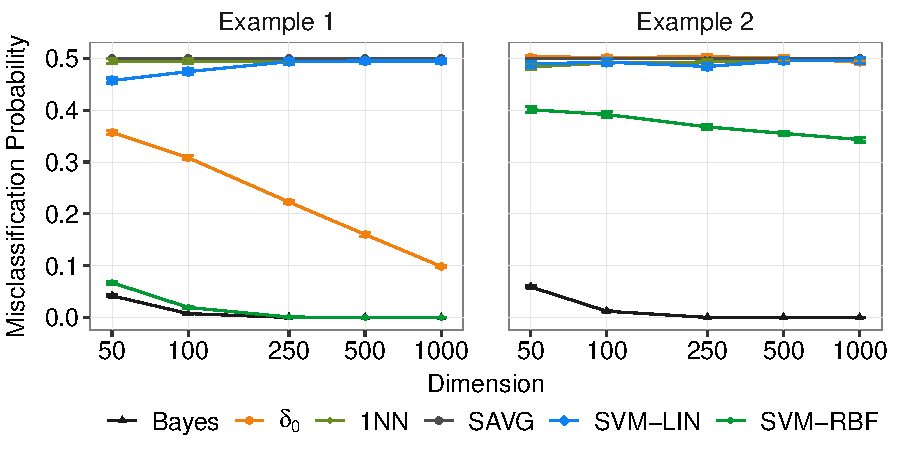
\includegraphics[width = 0.475\textwidth, height = 0.25\textwidth]{intro_plot_split1-2.pdf}
%   \vspace{.3in}
\caption{Average Misclassification Rates (along with Standard Errors) of $\delta_0$ and Some Popular Classifiers Based on 100 Replications.}
  \label{plot0}
\end{figure}
\vspace{-0.5cm}
In the first example, $\nu^2=0$ (since $\bmu_{1}=\bmu_{2}=\1_p$) but $\sigma^2_1=1$ and $\sigma^2_2=2$. The classifier $\delta_0$ indentifies this difference in scales and yields a moderate performance. Whereas existing classifiers (except SVM-RBF) misclassify 50\% of the observations. %whereas the Bayes risk goes to 0 as $p\to\infty$.
SVM-RBF capitalizes on the difference between $\sigma^2_1$ and $\sigma^2_2,$ and perfectly classifies the test observations as dimension increases. {\bf Example 2} poses a more challenging classification problem. Here, we have $\nu^2=0$ (since $\bmu_{1}=\bmu_{2}=\0_p$) and $\sigma_1^2=\sigma_2^2 = 3$, i.e., there is no difference between either of the location and scale parameters. As a result, the classifier $\delta_0$ as well as the existing classifiers fail to correctly classify the test observations. We will revisit these examples again in Sections \ref{d1vsd2} and \ref{sim}.
\subsection{Our Contribution}
In this article, we develop classifiers that are suitable for high dimensional data. The behavior of the proposed classifiers in HDLSS settings do not depend on the existence of the moments. %constants $\nu^2,\sigma_1^2$ and $\sigma_2^2,$or any relationship among them.
If the one-dimensional marginals of the underlying populations are different, then the proposed classifiers are shown to yield {\em perfect classification} in the HDLSS setting.
\vspace{-0.1cm}
\begin{tcolorbox}[colback=white]
The proposed  classifiers
\begin{itemize}
 %\item classify an observation correctly even when the competing class distributions have same location and scale,
 \vspace{-0.2cm}
 \item are robust,
 \vspace{-0.2cm}
 \item computationally fast,
 \vspace{-0.2cm}
 \item free from tuning parameters, and
 \vspace{-0.2cm}
 \item have strong theoretical properties.
\end{itemize}
\end{tcolorbox}
\vspace{-0.1cm}
The rest of the article is organized as follows. In Section \ref{method}, we propose a classifier and further modify it to achieve improved classification accuracy under specific conditions. Asymptotic properties of the proposed classifiers are studied in Section~\ref{asymptotics}. A theoretical result is presented in Section \ref{d1vsd2} to analyze their relative performances. In Section \ref{asym.uh}, we investigate their behavior when both $n$ and $p$ increase. Numerical performance of the proposed classifiers is studied using several simulated data sets in Section \ref{sim}. We also examine the behavior of our classifiers on some real data sets in Section \ref{real}. The article ends with some concluding remarks in Section \ref{conclude}. All proofs and relevant mathematical details are provided in Supplementary \ref{supA}. Additional details of our numerical study, and a link to related {\tt R} codes can be found in Supplementary \ref{supB}.

\section{METHODOLOGY}\label{method}

Let us recall the classifier $\delta_0$ stated in Section \ref{intro.motiv}. Fix $\bz\in\mathbb{R}^p.$ For given random samples $\rchi_1$ and $\rchi_2$ with sizes $n_1$ and $n_2$, respectively, the classifier $\delta_0$ is formally defined as
\begin{align}\label{d0def}
&\delta_0(\bz)=\argmin\limits_{j\in\{1,2\}} L_{j}(\bz),\text{ where }L_{j}(\bz) = T_{jj} - 2T_{j}(\bz),\nonumber\\
&T_{jj}  = \frac{1}{{n_j(n_j-1)}}\mathop{\sum\sum}\limits_{\substack{\bU,\bU^\prime\in\rchi_j,\\\bU\neq\bU^\prime}} h(\bU,\bU^\prime) \text{ and}\nonumber \\
&T_{j}(\bz) =\frac{1}{n_j}\sum\limits_{\bU\in\rchi_j}h(\bU,\bz)\text{ for } j=1,2.
\end{align}
\begin{comment}
Observe that
\begin{align*}
 &\ {\rm E}\ T_{1}(\bZ)\mid \bZ\sim\bF_1=  {\rm E}\ h(\bX_1,\bX_2),\\
 &\ {\rm E}\ T_{2}(\bZ)\mid \bZ\sim\bF_1=  {\rm E}\ h(\bX_1,\bY_1).\\
 Similarly, &\ {\rm E}\ T_{1}(\bZ)\mid \bZ\sim\bF_2=  {\rm E}\ h(\bX_1,\bY_1),\\
 \text{ and }&\ {\rm E}\ T_{2}(\bZ)\mid \bZ\sim\bF_2=  {\rm E}\ h(\bY_1,\bY_2)
\end{align*}
Therefore, it follows from \eqref{taudef} that an unbiased estimator of $\tau$ is $T = T_{11} + T_{22}- 2T_{12}$. We denote the expectations ${\rm E}\ h(\bX_1,\bX_2),{\rm E}\ h(\bX_1,\bY_1), {\rm E}\ h(\bY_1,\bY_2)$ by $\tau_{11} ,\tau_{12}$ and $\tau_{22}$ respectively, and express $\tau$ as $\tau = \tau_{11} + \tau_{22}- 2\tau_{12}$.
\end{comment}

In the previous section, we introduced the constants $\nu^2,\sigma_1^2$ and $\sigma_2^2$. Now, we define $\nu_{jj^\prime} = \lim_{p\to\infty}\bmu_j^\top\bmu_{j^\prime}/p$ for $j,j^\prime\in \{1,2\}$
\begin{comment}
 \begin{align}\label{limconst}
 &\nu_{11} = \frac{1}{p}\lim\limits_{p\to\infty}\bmu_1^\top\bmu_1,\ \nu_{12} = \frac{1}{p}\lim\limits_{p\to\infty}\bmu_1^\top\bmu_2,\nonumber \\
 &\nu_{22} = \frac{1}{p}\lim\limits_{p\to\infty}\bmu_2^\top\bmu_2,
\end{align}
\end{comment}
and further assume the following:
\begin{enumerate}
\item[(i)] There exists a constant $C_0$ such that ${\rm E}[|U_k|^4]<C_0<\infty$ for all $1\le k\le p,$ where $\bU=(U_1,\ldots,U_p)^\top\sim\bF_j$ for $j=1,2$.
\item[(ii)] The constants $\nu_{jj^\prime}$ and $\sigma^2_j$ exist for $ j,j^\prime\in\{1,2\}$.
\end{enumerate}

% \noindent (a). ${\rm E}|U_k|^4<C<\infty$ for all $1\le k\le p$ where $\bU\sim\bF_j$ are finite for $j=1,2$.
%\end{enumerate}
%\vspace{-0.2cm}

Let $\bU$ and $\bV$ be two independent vectors such that $\bU\sim\bF_j$ and $\bV\sim\bF_{j^\prime}$ for $j,j^\prime\in\{1,2\}$. We also assume that the components of the sequence $\{U_kV_k,k\geq 1\}$ are weakly dependent. In particular,
\begin{enumerate}
\item[(iii)] $\mathop{\sum\sum}\limits_{1\leq k<k^\prime\leq p}{\rm Corr}(U_kV_k, U_{k^\prime}V_{k^\prime})=o(p^2)$.
\end{enumerate}

Assumption (iii) is trivially satisfied if the component variables of the underlying populations are independent. It continues to hold with some additional conditions on their dependence structure. For example, (iii) is satisfied when the sequence $\{U_kV_k,k\geq 1\}$ has $\rho$-mixing property \citep{bradley2005basic, HMN05}. Conditions similar to (iii) are frequently considered in the literature for studying high-dimensional behavior of various statistical procedures \citep{ASSYZM18}.

\begin{lemma}\label{tau0def}
Suppose assumptions {\rm (i)-(iii)} are satisfied. For a test observation $\bZ,$ we define $L(\bZ) =L_2(\bZ) - L_1(\bZ).$
\begin{enumerate}[(a)]
\item  $\begin{aligned}[t]&\text{If }\bZ\sim\bF_1,\text{ then }
|L(\bZ) - {\tau}|\stackrel{\rm P}{\to}0\text{ as } p\to\infty .
 \end{aligned}$
\item  $\begin{aligned}[t]&\text{If }\bZ\sim\bF_2,\text{ then }
 |L(\bZ) + {\tau}|\stackrel{\rm P}{\to}0\text{ as } p\to\infty.
 \end{aligned}$
\end{enumerate}
%  \vspace{-0.2cm}
%  \begin{align*}
%  \vspace{-0.2cm}
% &\text{where }\bU\sim\bF_i,\text{ and }\bV\sim\bF_{j}\text{ for }j,j^\prime\in\{1,2\}.
%  \end{align*}
\end{lemma}
Lemma \ref{tau0def} states that if $\bZ\sim\bF_1$ (respectively, $\bZ\sim\bF_2$), then the discriminant corresponding to $\delta_0$ converges in probability to $\tau,$ a positive (respectively, negative) quantity as $p\to\infty$. The misclassification probability of a classifier $\delta$ is defined as $\Delta=\pi_1{\rm P}[\delta(\bZ)=2|\bZ\sim\bF_1]+\pi_2{\rm P}[\delta(\bZ)=1|\bZ\sim\bF_2].$ Here $\pi_j>0$ is the prior probability of $j$-th class for $j=1,2$ with $\pi_1+\pi_2=1.$ %Throughout this article, we will follow this definition of the misclassfication probability $\Delta$.
Let $\Delta_0$ denote the misclassification probability of the classifier $\delta_0.$ The following theorem shows that the asymptotic behavior of $\delta_0$ is governed by the constants $\nu_{jj^\prime}$ and $ \sigma^2_j$ for $j,j^\prime\in\{1,2\}$ in HDLSS settings.
\begin{thm}\label{theorem0}
Suppose that assumptions {\rm (i)-(iii)} are satisfied, and either of the following two conditions hold:
\begin{enumerate}[(a)]
\vspace{-0.35cm}
 \item $\nu_{11}, \nu_{12}$ and $\nu_{22}$ are unequal, %(i.e., $\nu^2>0$),
 \vspace{-0.25cm}
\item $\nu_{11}= \nu_{12} = \nu_{22}\neq 0$ and $\sigma_1^2 \neq \sigma_2^2$.
\vspace{-0.35cm}
\end{enumerate}
For any $\pi_1>0$, $\Delta_0\to 0$ as $p\to\infty $.
\end{thm}
% \vspace{-0.2cm}
% Note that if neither (a) nor (b) is satisfied, then $\tau_0=0$. Consequently, following Lemma \ref{tau0def} we conclude that the discriminant $L_2(\bZ)-L_1(\bZ)$ converges to 0 irrespective of the class label of $\bZ$, and thus $\delta_0$ becomes useless.
It follows from Theorem \ref{theorem0} that if $\bF_1$ and $\bF_2$ differ either in their locations and/or scales, then $\Delta_0$ converges to 0 as dimension increases. Recall {\bf Example \ref{ex1}}, and note that condition $(b)$ of Theorem \ref{theorem0} is satisfied  in this example since $|\sigma^2_1-\sigma^2_2|=1$. In {\bf Example \ref{ex2}}, both $(a)$ and  $(b)$ are violated and  Theorem \ref{theorem0} fails to hold. This gives us a clear explanation why the classifier $\delta_0$ performed well in the first example, but failed in the second one (see Figure \ref{plot0}). We now develop some classifiers whose asymptotic properties are not governed by the constants $\nu_{jj^\prime},$ and $ \sigma^2_j$ for $j,j^\prime\in\{1,2\}.$ The proposed classifiers use differences between the one-dimensional marginals of $\bF_1$ and $\bF_2$, and attain {\it perfect classification} in high dimensions under fairly general conditions.

\subsection{A New Measure of Distance}\label{AoDist}
Let $F_{j,k}$ denote the distribution of the random variable $U_k,$ where $\bU=(U_1,\ldots, U_{p})^\top\sim\bF_j$ for $j=1,2$ and $1\le k\le p.$
%If $\bX=$ $(X_1,\ldots,X_p)^\top\sim\bF_1$ and $\bY=$ $(Y_1,\ldots,Y_p)^\top\sim\bF_2$, then we denote the distribution of $X_k$ and $Y_k$ by $F_{1,k}$ and $F_{2,k}$, respectively, for $1\le k\le p$.
Suppose that $\bX_1,\bX_2\stackrel{i.i.d.}{\sim}\bF_1$ and $\bY_1,\bY_2\stackrel{i.i.d.}{\sim}\bF_2$. Fix $1\le k\le p$ and recall the definition of $\tau$ stated in Section \ref{intro.motiv}. The distance between $F_{1,k}$ and $F_{2,k}$ is given by $\tau_k = {\rm E}\big [ h(X_{1k},X_{2k})-2 h(X_{1k},Y_{1k})+ h(Y_{1k},Y_{2k})\big ]$. Here, $\tau_k\geq 0$ and equality holds iff $F_{1,k}=F_{2,k}.$ We denote the average of these distances by $\bar{\tau}_p=\sum_{k=1}^{p}\tau_k/p$. Clearly,
$\bar{\tau}_p=0$ iff $\tau_k=0$ for all $1\le k\le p$,
% \begin{tcolorbox}[colback = white]
$$\text{i.e., }\bar{\tau}_p=0\text{ iff }F_{1,k}=F_{2,k}\text{ for all }1\le k\le p.$$
% \end{tcolorbox}
This property of $\bar{\tau}_p$ suggests that it can be used as a {\it measure of separation} between $\bF_1$ and $\bF_2$. If $F_{1,k}\neq F_{2,k}$ for some $1\le k\le p,$  then $\bar{\tau}_p$ is strictly positive. This is the fundamental idea that we will use in constructing a new classifier.

Recall the definition of $h$ given in Section \ref{intro.motiv}, and consider
\vspace{-0.25cm}
\begin{align}\label{hbardef}
 & \bar{h}_p(\bu,\bv)= \frac{1}{p}\sum\limits_{k=1}^{p}h(u_k,v_k)\text{ for }\bu,\bv\in\mathbb{R}^p.
 %\text{i.e., }&\ \bar{h}(\bu,\bv)=\frac{1}{2\pi p}\sum\limits_{k=1}^{p}\sin^{-1}\frac{1+u_k v_k}{\sqrt{(1+u^2_k)(1+v^2_k)}}.
\end{align}
Using \eqref{hbardef}, we re-write the definition of $\bar{\tau}_p$ as
\begin{align*}
 &\bar{\tau}_p={\rm E}[ \bar{h}_p(\bX_{1},\bX_{2})-2 \bar{h}_p(\bX_{1},\bY_{1}) +  \bar{h}_p(\bY_{1},\bY_{2})].
\end{align*}
Let $\bar{\tau}_p(1,1),\bar{\tau}_p(1,2)(=\bar{\tau}_p(2,1))$ and $\bar{\tau}_p(2,2)$ denote the quantities ${\rm E} [\bar{h}_p(\bX_{1},\bX_{2})]$, ${\rm E}[\bar{h}_p(\bX_{1},\bY_{1})]$ and ${\rm E}[\bar{h}_p(\bY_{1},\bY_{2})$, respectively. Observe that
\vspace{-0.2cm}
\begin{align}\label{altdeftaubar}
 \bar{\tau}_p=\bar{\tau}_p(1,1)- 2\bar{\tau}_p(1,2) + \bar{\tau}_p(2,2).
\end{align}
Fix $\bz\in\mathbb{R}^p.$ Define the following:
\begin{align}\label{barLdef}
&{\bar{T}}_{jj}  = \frac{1}{n_j(n_j-1)}\mathop{\sum\sum}\limits_{\substack{ \bU,\bU^\prime\in\rchi_j \\ \bU\neq\bU^\prime}}\bar{h}_p(\bU,\bU^\prime),\nonumber\\
&\bar{T}_{j}(\bz) = \frac{1}{n_j}\sum\limits_{\bU\in\rchi_j}\bar{h}_p(\bU,\bz),\nonumber\\
& \bar{L}_j(\bz) = \bar{T}_{jj} - 2\bar{T}_{j}(\bz)\text{ for } j=1,2\nonumber\\
&\text{and }\bar{L}(\bz)=\bar{L}_{2}(\bz) - \bar{L}_{1}(\bz).
\end{align}
% \vspace{-0.25cm}
\noindent It follows from the above definitions that
\begin{align}\label{estexpect}
 &{\rm E}[ \bar{T}_{j}(\bZ)\mid\bZ\sim\bF_{j^\prime}]=\bar{\tau}_p(j,j^\prime)\text{ and}\nonumber \\
 &{\rm E}[ \bar{T}_{jj}]=\bar{\tau}_p(j,j)\text{ for }j,j^\prime\in\{1,2\} .
\end{align}
\noindent Consequently, we obtain
% \vspace{-0.1cm}
\begin{align}\label{motiv}
 &{\rm E}[ \bar{L}(\bZ) \mid\bZ\sim\bF_1] = \bar{\tau}_p\geq 0\text{ and}\nonumber \\
 &{\rm E}[ \bar{L}(\bZ) \mid\bZ\sim\bF_2] = -\bar{\tau}_p\leq 0.
\end{align}
It is clear from this equation that ${\rm E}[\bar{L}(\bZ)]$ indicates whether a test observation $\bZ$ belongs to the first, or the second class. This key observation motivates us to use $\bar{L}(\bZ)$ as the discriminant of our classifier.
\subsubsection{A Classifier Based on $\bar{\tau}_p$}\label{method.taubar}
Using \eqref{motiv}, we propose the following classifier:
\begin{align}\label{delta1def}
 \delta_1(\bz)=\begin{cases}
                1,& \text{ if }\bar{L}(\bz)>0,\\
                2,& \text{ otherwise,}
               \end{cases}
\end{align}
The classifier $\delta_1$ can also be expressed as $\argmin_{j\in\{1,2\}}\bar{L}_j(\bz).$ For given random samples $\rchi_1, \ldots, \rchi_J$ (with $J>2$), we define $ \delta_1(\bz)=\argmin_{1\leq j\leq J}\bar{L}_j(\bz)$, where $\bar{L}_j(\bz),$ $\bar{T}_j(\bz)$ and $\bar{T}_{jj}$ are as defined in \eqref{barLdef} for $1\le j\le J$. The misclassification probability of $\delta_1$ is denoted by $\Delta_1$.

\subsection{Limitations of Using $\bar{\tau}_p$}\label{method.taubarlim}
To classify a test point, the classifier $\delta_1$ leverages on the quantity $\bar{\tau}_p$, the average of distances between $F_{1,k}$ and $F_{2,k}$ for $1\le k\le p.$ However, $\bar{\tau}_p$ has some limitations. Recall that
\begin{align*}
 \bar{\tau}_p& =\ \bar{\tau}_p(1,1) - 2\bar{\tau}_p(1,2) + \bar{\tau}_p(2,2)\\
 &=\ \{\bar{\tau}_p(1,1) - \bar{\tau}_p(1,2)\}+\{\bar{\tau}_p(2,2) - \bar{\tau}_p(1,2)\}.
\end{align*}
Since $\bar{\tau}_p\geq 0$, we always have $\bar{\tau}_p(1,2)\leq \{\bar{\tau}_p(1,1) + \bar{\tau}_p(2,2)\}/2$. Without loss of generality, let us assume that $\bar{\tau}_p(1,1)< \bar{\tau}_p(2,2)$. If $\bar{\tau}_p(1,2)$ lies between $\bar{\tau}_p(1,1)$ and $\bar{\tau}_p(2,2),$ i.e., $\bar{\tau}_p(1,1) < \bar{\tau}_p(1,2)<\bar{\tau}_p(2,2) $, then $\bar{\tau}_p(1,1) - \bar{\tau}_p(1,2)<0$ and $\bar{\tau}_p(2,2) - \bar{\tau}_p(1,2)>0.$ Adding them up may cancel each other. As a result, $\bar{\tau}_p$ may not fully capture the difference between $\bF_1$ and $\bF_2.$ % despite $\bF_{1}$ and $\bF_{2}$ being different.
One way to rectify this problem is to square the two quantities before adding them up. %This will eliminate the possibility of cancellations.
Define
\begin{align*}%\label{psibardef0}
 \bar{\psi}_p = \{\bar{\tau}_p(1,1) - \bar{\tau}_p(1,2)\}^2+\{\bar{\tau}_p(2,2) - \bar{\tau}_p(1,2)\}^2.
\end{align*}
It is easy to check that
$\bar{\psi}_p=0\text{ iff }F_{1,k}=F_{2,k}\text{ for all }1\le k\le p.$ Hence, $\bar{\psi}_p$ can also be viewed as a measure of separation between $\bF_1$ and $\bF_2.$ This new measure can also be expressed as
\begin{align}\label{psibardef}
 \bar{\psi}_p=\frac{1}{2}\big [\bar{\tau}_p^2 +\{\bar{\tau}_p(1,1) - \bar{\tau}_p(2,2)\}^2\big ].\vspace{-0.175cm}
\end{align}
Observe that if $\bar{\tau}_p(1,2)$ lies between $\bar{\tau}_p(1,1)$ and $\bar{\tau}_p(2,2),$ then $|\bar{\tau}_p(1,1)-\bar{\tau}_p(2,2)|> \bar{\tau}_p.$ As a result,
$$\bar{\psi}_p=\frac{1}{2}\big [\bar{\tau}_p^2 +\{\bar{\tau}_p(1,1) - \bar{\tau}_p(2,2)\}^2\big ]> \frac{1}{2}\big [\bar{\tau}_p^2 +\bar{\tau}_p^2]=\bar{\tau}_p^2.$$
On the other hand, if $\bar{\tau}_p(1,2)$ is smaller than both $\bar{\tau}_p(1,1)$ and $\bar{\tau}_p(2,2),$ then $\bar{\psi}_p< \bar{\tau}^2_p.$ If $\bar{\psi}_p> \bar{\tau}^2_p$, then $\bar{\psi}_p$ is a better choice than $\bar{\tau}_p$ in terms of measuring separation between two distributions. %Clearly, $\bar{\tau}_p\ge 1$ implies $\bar{\psi}_p> \bar{\tau}_p,$.
In general, if the underlying distributions $\bF_1$ and $\bF_2$ are such that $\bar{\tau}_p(1,2)>\min\{\bar{\tau}_p(1,1),\bar{\tau}_p(2,2)\},$ then a classifier that utilizes $\bar{\psi}_p$ is shown to have better classification accuracy than the classifier $\delta_1$ (see Section \ref{d1vsd2} for more details). The modification proposed in \eqref{psibardef} is similar to what \cite{biswas2014nonparametric} had suggested for improving the power of some energy based tests for HDLSS data.
\subsubsection{A Classifier Based on $\bar{\psi}_p$}\label{method.improvclass}
We now develop a classifier that leverages the amplified measure of dissimilarity $\bar{\psi}_p.$ First, we estimate $\bar{\tau}_p(1,2)$ as follows:
% \vspace{-0.2cm}
\begin{align}\label{T12def}
{\bar{T}}_{12} =\frac{1}{n_1n_2}\sum\limits_{ i=1}^{n_1}\sum\limits_{ j=1}^{n_2}\bar{h}_p(\bX_i,\bY_j).
\vspace{-0.35cm}
\end{align}
% \vspace{-0.2cm}
%We intend to construct a discriminant that converges to $\bar{\psi}_p$ (respectively, $-\bar{\psi}_p$) as $p\to\infty$ if $\bZ\sim\bF_1$ (respectively, $\bZ\sim\bF_2$).
Fix $\bz\in\mathbb{R}^p$. Define
\begin{align}\label{thetabardef}
\hspace{-0.25cm}\bar{\theta}(\bz) =&\frac{1}{2}\big\{\bar{T}_{11}-2\bar{T}_{12}+\bar{T}_{22}\big\}\big\{\bar{L}_2(\bz)-\bar{L}_1(\bz)\big\}\nonumber \\
 +& \frac{1}{2}\big\{\bar{T}_{22}-\bar{T}_{11}\big\}\big\{\bar{L}_2(\bz)+\bar{L}_1(\bz)+2\bar{T}_{12}\big \}.
\end{align}
We will prove that $|\bar{\theta}(\bZ)|$ is a consistent estimator of $\bar{\psi}_p,$ where $\bZ$ is a test observation. In particular, $\bar{\theta}(\bZ)$ converges in probability to $\bar{\psi}_p$ as $p\to\infty$ if $\bZ\sim\bF_1,$ and to $-\bar{\psi}_p$ if $\bZ\sim\bF_2$ (see Lemma \ref{L2}).
\begin{comment}
Define $\bar{T} = \bar{T}_{11}-2\bar{T}_{12}+\bar{T}_{22}$. From\eqref{estexpect}, we have ${\rm E}[\bar{T}] = \bar{\tau}_p>0$. Also note that ${\rm E}[\bar{L}_2(\bZ)-\bar{L}_1(\bZ)] = \bar{\tau}_p\text{ (resp., }-\bar{\tau}_p)$ if $\bZ\sim\bF_1$ (resp., $\bZ\sim\bF_2$). We show that $\bar{T}\{\bar{L}_2(\bZ)-\bar{L}_1(\bZ)\}$ converges to $\bar{\tau}_p^2\text{ (or, }-\bar{\tau}_p^2)$ as $p\to\infty$, when $\bZ\sim\bF_1\text{ (or, }\bZ\sim\bF_2)$. Similarly, following  \eqref{barLdef}-\eqref{motiv}, we show that $\big\{\bar{T}_{22}-\bar{T}_{11}\big\}\big\{\bar{L}_2(\bZ)+\bar{L}_1(\bZ)+2\bar{T}_{12}\big \}$  converges to $(\bar{\tau}_{22}-\bar{\tau}_{11})^2$ (or, $-(\bar{\tau}_{22}-\bar{\tau}_{11})^2$) as $p\to\infty$, if $\bZ\sim\bF_1$ (or, $\bZ\sim\bF_2$).
Note that one can obtain the following from  \eqref{barLdef} and \eqref{estexpect}:
\begin{align*}
 &{\rm E}[\bar{T}_{11}-2\bar{T}_{12}+\bar{T}_{22}] = \bar{\tau}_p,\\
 &{\rm E}[\bar{T}_{22}-\bar{T}_{11}] = \bar{\tau}_p(2,2) - \bar{\tau}_p(1,1),\\
 &{\rm E}[\bar{L}_2(\bZ)+\bar{L}_1(\bZ) + 2\bar{\tau}_p(1,2)\mid \bZ\sim\bF_1] = \bar{T}_{22}-\bar{T}_{11},\\
 &{\rm E}[\bar{L}_2(\bZ)+\bar{L}_1(\bZ) + 2\bar{\tau}_p(1,2)\mid \bZ\sim\bF_2] = \bar{T}_{11}-\bar{T}_{22}.
\end{align*}
Combining the above equations with \eqref{motiv},
To summarize, $\bar{\theta}(\bZ)$ is expected to take positive (or, negative) values if $\bZ\sim\bF_1$ (or, $\bZ\sim\bF_2$).
\end{comment}
This motivates us to construct the following classifier:
\vspace{-0.1cm}
\begin{align}\label{del2def}
 \delta_2(\bz)=\begin{cases}
                1,& \text{ if }\bar{\theta}(\bz)>0,\\
                2,& \text{ otherwise.}
               \end{cases}
\end{align}
Let $\Delta_2$ denote the misclassfication probability of the classifier $\delta_2.$ Unlike $\delta_1$, the classifier $\delta_2$ cannot be readily extended to deal with $J$ class problems when $J>2$. For multi-class problems, we implement the idea of `majority voting' \citep{friedman2001elements}.% to classify a new observation $\bz$ when $J> 2$.

{\bf Examples 1} and {\bf 2} establish the advantage of using $\delta_2$ over $\delta_1.$ In Figure \ref{plot1}, we see that $\delta_2$ has substantial improvement over $\delta_1$ in terms of misclassfication probability. This improvement stems from the fact
\begin{figure}[H]
  \centering
    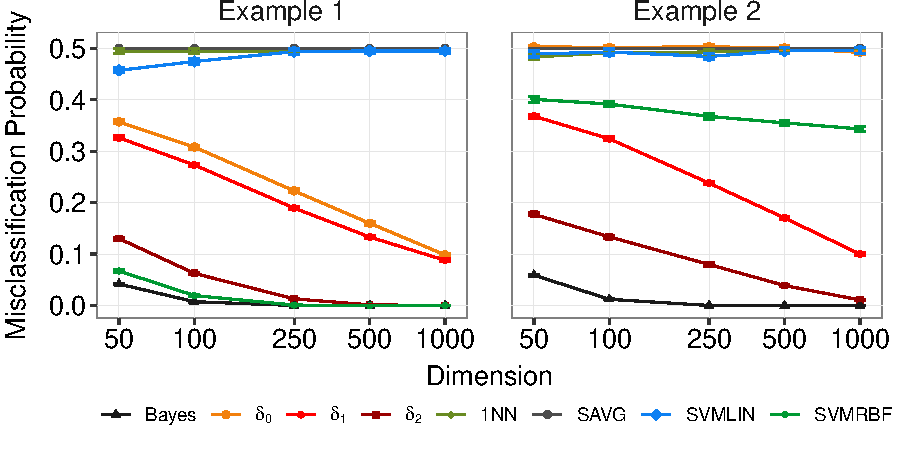
\includegraphics[width = 0.475\textwidth, height = 0.235\textwidth]{section2_plot_split1-2.pdf}
   %\vspace{.3in}
 \caption{Average Misclassification Rates (along with Standard Errors) of the Proposed Classifiers Are Plotted Based on 100 Replications.}
  \label{plot1}
\end{figure}
that $\bar{T}_{12}$ lies between $\bar{T}_{11}$ and $\bar{T}_{22}$ in both examples (see Table \ref{order.d1.d2} in Supplementary \ref{supB}). A theoretical result on the relative performance of these two classifiers is presented in Section \ref{d1vsd2}.

\section{ASYMPTOTIC PROPERTIES}\label{asymptotics}
In HDLSS settings, $n$ is fixed and $p\to\infty$, whereas in the  \emph{ultrahigh-dimensional} setting, $p$ grows simulatenously with $n$. The behavior of the classifiers  $\delta_1$ and $\delta_2$ is investigated in both aymptotic regimes. We first show that the classifiers yield {\it perfect classification} in HDLSS settings under fairly general conditions.
\subsection{Asymptotic Behavior in HDLSS Settings}\label{asymp.HDLSS}
Suppose $\bU$ and $\bV$ are two independent vectors such that $\bU=(U_1,\ldots, U_p)^\top\sim \bF_j$ and $\bV=(V_1,\ldots, V_p)^\top\sim \bF_{j^\prime}$ for $j,j^\prime\in\{1,2\}$. We assume that the component variables are weakly dependent. In particular, we assume
\begin{enumerate}
 \item[A1.] $\mathop{\sum\sum}\limits_{1\leq k<k^\prime\leq p}{\rm Corr}(h(U_k,V_k), h(U_{k^\prime},V_{k^\prime}))=o(p^2)$,
\end{enumerate}
where $h$ is defined in Section \ref{intro.motiv}. Assumption A1 is trivially satisfied if the component variables of the underlying distributions are independently distributed and it continues to hold when the components have weak dependence among them. For example, A1 is satisfied when the sequence $\{h(U_k,V_k),k\geq 1\}$ has $\rho$-mixing property. Note that if the sequences $\{U_k,k\geq 1\}$ and $\{V_k,k\geq 1\}$ have $\rho$-mixing property, then $\{h(U_k,V_k),k\geq 1\}$ has $\rho$-mixing property for every measurable function $h$ (see Theorem 6.6-II of \cite{bradley2007introduction}).

Recall assumption (iii) introduced in Section \ref{method}. Both (iii) and A1 require the component variables to be weakly dependent. However, A1 is weaker between the two since, unlike (iii), it does not require existence of the first and second order moments. Observe that the function $h$ is bounded. Thus, assumption A1 holds even if the underlying distributions are heavy-tailed.

% \vspace{-0.15cm}
\begin{lemma}\label{L2}
 If {\rm A1} is satisfied, then for a test observation $\bZ$, we have
%  \vspace{-0.1cm}
%\begin{small}
\begin{enumerate}[(a)]
\item  $\begin{aligned}[t]&\text{If }\bZ\sim\bF_1,\text{ then }
|\bar{L}(\bZ) - \bar{\tau}_p|\stackrel{\rm P}{\to}0\text{ and}\\
&|\bar{\theta}(\bZ)-\bar{\psi}_p|\stackrel{\rm P}{\to}0\text{ as } p\to\infty .
 \end{aligned}$
%\end{small}
%\vspace{-0.15cm}
\item  $\begin{aligned}[t]&\text{If }\bZ\sim\bF_2,\text{ then }
 |\bar{L}(\bZ) + \bar{\tau}_p|\stackrel{\rm P}{\to}0\text{ and}\\
    &|\bar{\theta}(\bZ)+\bar{\psi}_p|\stackrel{\rm P}{\to}0\text{ as } p\to\infty.
 \end{aligned}$
\end{enumerate}
\end{lemma}
% \vspace{-0.15cm}
This lemma shows that assumption A1 is sufficient for convergence of the discriminants $\bar{L}(\bZ)$ and $\bar{\theta}(\bZ)$. Similar results on distance concentration can be derived for independently distributed sub-Gaussian components (see Theorem 3.1.1 of \cite{vershynin2018high} for further details). Lemma \ref{L2} is stronger than existing results in the sense that it holds even when the components are not necessarily independent, or sub-Gaussian.

Lemma \ref{L2} states that both the discriminants converge in probability to a non-negative value if $\bZ\sim\bF_1$, while they converge in probability to a value which is not positive when $\bZ\sim\bF_2$. Now, we expect $\delta_1$ and $\delta_2$ to yield good performance if $\bar{\tau}_p$ and $\bar{\psi}_p$ do not vanish with increasing dimension. Clearly, $\bar{\tau}_p=\bar{\psi}_p=0$ iff $F_{1,k}=F_{2,k}$ for all $1\le k\le p$. Hence, it is reasonable to assume the following:
\begin{enumerate}
 \item[A2.] $\liminf\limits_{p} \bar{\tau}_p>0$.
\end{enumerate}
A2 implies that the separation between $\bF_1$ and $\bF_2$ is asymptotically non-negligible. Observe that this assumption is satisfied if the component variables of $\bU\sim\bF_j$ are identically distributed for $j=1,2$. In this case, $\tau_{k}=\tau_1>0$ for all $k\ge 1$, making $\bar{\tau}_p(=\tau_1)$ free of $p$. It follows from the definition of $\bar{\psi}_p$ in \eqref{psibardef} that A2 also implies $\liminf_p\bar{\psi}_p>0$.

\subsubsection{Asymptotic Properties of $\delta_1$ and $\delta_2$ in HDLSS Settings}\label{asym.HDLSS.d1d2}

We now discuss the behavior of the classifiers $\delta_1$ and $\delta_2$ in HDLSS settings. We show that under fairly general conditions, the proposed classifiers $\delta_1$ and $\delta_2$ perfectly classify a test observation as the dimension increases.
\begin{thm}\label{d1thm}
 If {\rm A1} and {\rm A2} are satisfied, then for any $\pi_1>0$,
 \begin{enumerate}[(a)]
  \item $\Delta_1\to 0$ as $p\to\infty ,$ and
  \item $\Delta_2\to 0$ as $p\to\infty $.
 \end{enumerate}
\end{thm}
Observe that the asymptotic behavior of the classifiers are no longer governed  by the constants $\nu_{jj^\prime}$ and $\sigma^2_j$ for $j,j^\prime\in\{1,2\}$. In fact, their behavior do not depend on the existence of moments. In this sense, the classifiers $\delta_1$ and $\delta_2$ are robust.
\begin{tcolorbox}[colback=white]
Asymptotic behavior of the proposed classifiers is free of moment conditions.\newline

The classifiers yield {\it perfect classificaton} under quite weak conditions.%an observation if the underlying populations $\bF_1$ and $\bF_2$ have asymptotically non-zero separation and components are weakly dependent.
\end{tcolorbox}
One should observe that assumptions A1 and A2 are fairly general, and Theorem \ref{d1thm} is stronger than what currently exists in the literature.

\subsubsection{Comparison Between $\delta_1$ and $\delta_2$}\label{d1vsd2}
It is clear from Theorem \ref{d1thm} that both the classifiers yield {\it perfect classification} under the same set of assumptions. The next result provides a set of sufficient conditions under which one classifier performs better than the other.

First, let us consider the following assumption:
\begin{enumerate}
 \item[A3.] There exists a $p_0\in\mathbb{N}$ such that $\bar{\tau}_p(1,2)>\min\{\bar{\tau}_p(1,1),\bar{\tau}_p(2,2)\}$ for all $p\ge p_0.$
\end{enumerate}
If assumption A3 is satisfied, then either $\bar{\tau}_p(1,1)-\bar{\tau}_p(1,2)$ or $\bar{\tau}_p(2,2)-\bar{\tau}_p(1,2)$ is positive, while the other one is negative.
So, $\bar{\tau}_p$ may take a small value (recall the discussion in Section \ref{method.taubarlim}). The next result suggests that under such circumstances, $\delta_2$ leads to an improve performance over $\delta_1.$
\begin{thm}\label{cmpr_d1_d2}
If assumptions ${\rm (A1)}-{\rm (A3)}$ are satisfied, then there exists an integer $p^\prime_0$ such that
$$\Delta_{2} \leq \Delta_{1} \text{ for all } p\geq p^\prime_0.$$
\end{thm}
%If $\bar{\tau}_p(1,2)$ and $\min\{\bar{\tau}_p(1,1),\bar{\tau}_p(2,2)\}$ are interchanged in
If the inequality stated in assumption A3 is inverted, then the ordering of $\Delta_1$ and $\Delta_2$ in Theorem \ref{cmpr_d1_d2} is reversed. Note that $\bar{T}_{11} ,\bar{T}_{12}$ and $\bar{T}_{22}$ are unbiased estimators of $\bar{\tau}_p(1,1) ,\bar{\tau}_p(1,2)$ and $\bar{\tau}_p(2,2),$ respectively (see \eqref{estexpect}). We now use these estimators to explain the relative performance of the proposed classifiers. In {\bf Examples 1} and {\bf 2}, $\bar{T}_{12}$ lies in  between $\bar{T}_{11}$ and $\bar{T}_{22}$ (see Table \ref{tab3} in Supplementary \ref{supB}). Following Theorem \ref{cmpr_d1_d2}, we expect $\Delta_2$ to be smaller than $\Delta_1$ in these examples. Figure \ref{plot1} shows that the estimated misclassfication probability of the classifier $\delta_2$ is indeed smaller than that of $\delta_1$ in both examples.

\subsection{Asymptotic Properties of $\delta_1$ and $\delta_2$ for Increasing Sample Size}\label{asym.uh}
In this section, we assess the performance of our classifiers in the {\it ultrahigh-dimensional} asymptotic regime, when the dimension $p\ (\equiv p_n)$ is allowed to grow with $n$ (in non-polynomial order). In particular, we assume the following:
\begin{enumerate}
 \item[A4.] There exists $\beta\ge 0$ such that $\log \ p_n=O(n^\beta).$
\end{enumerate}
Recall that in the classical asymptotic regime, $p$ is fixed and $n\to\infty$. Therefore, the classical setting is a special case of the \emph{ultrahigh-dimensional} regime with $\beta=0$. Also, assume that $\lim_{n\to\infty} n_1/n=\pi_1$.

We first present the `oracle' versions of our classiifiers when $\bF_1$ and $\bF_2$ are known. Fix $\bz\in\mathbb{R}^p.$ The `oracle' version of $\delta_1$ is defined as follows:
\begin{align}\label{oracle1def}
 \delta^0_1(\bz)=\begin{cases}
                1,& \text{ if }\bar{L}^0(\bz)>0,\\
                2,& \text{ otherwise,}
               \end{cases}
\end{align}
where $\bar{L}^0(\bz)=\bar{L}^0_2(\bz)-\bar{L}^0_1(\bz),$ with $\bar{L}^0_j(\bz) = \bar{\tau}_p(j,j) - 2{\rm E}[\bar{h}_p(\bU,\bz)]$ for $\bU\sim\bF_j$ and $ j=1,2.$ Similarly, we define $\delta^0_2$, the `oracle' version of $\delta_2$ as follows:
\begin{align}\label{oracle2def}
 &\delta^0_2(\bz)=\begin{cases}
                1,& \text{ if }\bar{\theta}^0(\bz)>0,\\
                2,& \text{ otherwise,}
               \end{cases}
\end{align}
where $2\bar{\theta}^0(\bz) =\bar{\tau}_p\bar{L}^0(\bz)+ \big\{\bar{\tau}_p(2,2)-\bar{\tau}_p(1,1)\big\} \times \big\{\bar{L}^0_2(\bz)+\bar{L}^0_1(\bz)+2\bar{\tau}_p(1,2)\big \}.\nonumber$ Note that $\bar{L}(\bz)$ and $\bar{\theta}(\bz)$ (defined in \eqref{barLdef} and \eqref{thetabardef}) are in fact estimators of $\bar{L}^0(\bz)$ and $\bar{\theta}^0(\bz),$ respectively. %Therefore, $\delta_j$ is an estimator of $\delta^0_j$ for $j=1,2.$ %Naturally, the due to error in estimation. Needless to say, it follows from Theorem \ref{d1thm} and \ref{d2thm} that $\Delta_i\to 0$ as $p\to\infty$ for $i=1,2.$\newline

Let $\Delta^0_j$ denote the misclassification probability of the classifier $\delta^0_j$ for $ j=1,2.$ In this section, we derive an upper bound on the difference $\Delta_j-\Delta^0_j$ for $j=1,2.$ Furthermore, we show that in the classical setting (i.e., $p$ is fixed), if the competing distributions are absolutely continuous, then $\Delta_j-\Delta^0_j$ converges to 0 for $j=1,2$ as $n\to\infty.$ We first look into convergence results for the discriminants $\bar{L}(\bz)$ and $\bar{\theta}(\bz).$ %The following lemma presents the rates at which the discriminants $\bar{L}(\bz)$ and $\bar{\theta}(\bz)$ converge in probability to their respective population counterparts, i.e, $\bar{L}^0(\bz)$ and $\bar{\theta}^0(\bz)$ as $n$ increases.
\begin{lemma}\label{exbdLtheta}
Suppose assumption {\rm A4} is satisfied for some $0\le \beta <1.$ For any $\pi_1 >0$ and $0<\gamma <(1-\beta)/2$, there exist positive constants $B_0$ and $B_1$ such that
\vspace{-0.25cm}
\begin{enumerate}[(a)]
 \item $ {\rm P}\big [|\bar{L}(\bz) - \bar{L}^0(\bz)|>n^{-\gamma}  \big]\leq O\left (e^{-B_0\{ n^{1-2\gamma}-n^\beta\}}\right ),$
 \item ${\rm P}\big [|\bar{\theta}(\bz) - \bar{\theta}^0(\bz)|>n^{-\gamma} \big]\leq O\left ( e^{-B_1\{ n^{1-2\gamma}-n^\beta\}}\right )$
\end{enumerate}
\vspace{-0.25cm}
for all $\bz\in\mathbb{R}^{p}.$
%  \vspace{-0.2cm}
% \end{small}
% \vspace{-0.5cm}
\end{lemma}
\vspace{-0.25cm}
Since $1-2\gamma>\beta,$ we have $e^{-\{n^{1-2\gamma}-n^\beta\}}\to 0$ as $n\to\infty.$ The above result shows that $|\bar{L}(\bz)-\bar{L}^0(\bz)|$ and $|\bar{\theta}(\bz)-\bar{\theta}^0(\bz)|$ converge to 0 at an exponential rate as $n$ increases. Using Lemma \ref{exbdLtheta}, we have the next result.
%\subsubsection{Large Sample Behavior of $\delta_1$ and $\delta_2$}\label{asym.uh.d1d2}
%In HDLSS asymptotic regime, we assumed that the distance between $\bF_1$ and $\bF_2$ does not vanish with increasing dimension. In ultrahigh-dimensional setting, we relax the condition and assume the following:

%A4. There exist $0<\alpha_1<(1-\beta)/2$ such that $1/\bar{\tau}_{p_n}=o(n^{\alpha_1})$.

%A4 allows $\bar{\tau}_{p_n}$ to decrease to 0, but at a rate slower than $n^{-\alpha_1}$ for an $0<\alpha_1<(1-\beta)/2$.
%\vspace{-0.1cm}
\begin{thm}\label{d1thmUH}
Suppose assumption {\rm A4} is satisfied for some $0\le \beta <1.$ For any $\pi_1 >0$ and $0<\gamma <(1-\beta)/2$, there exist positive constants $B_0$ and $B_1$ such that
 \vspace{-0.25cm}
 \begin{enumerate}[(a)]
  \item $ \Delta_1-\Delta^0_1\\
  \leq O\left (e^{-B_0\{n^{1-2\gamma}-n^\beta\}}\right )+ P\big [|\bar{L}^0(\bZ)|<n^{-\gamma}\big ],$
  \item $ \Delta_2-\Delta^0_2\\
  \leq O\left (e^{-B_1\{n^{1-2\gamma}-n^\beta\}}\right )+P\big [|\bar{\theta}^0(\bZ)|<n^{-\gamma}\big ].$
 \end{enumerate}
\end{thm}
\begin{comment}
Theorem \ref{d1thmUH} provides an upper bound to the difference between misclassification probabilities of the proposed classifiers and its corresponding oracle versions.
\begin{cor}\label{classical} If assumption {\rm A4} is satisfied with $\beta=0$ and $\bF_1,\bF_2$ are absolutely continuous, then $\Delta_1-\Delta^0_1$ and $\Delta_2-\Delta^0_2$ converge to 0 as $n\to\infty.$
\end{cor}
\end{comment}
Clearly, $e^{-B_0 \{n^{1-2\gamma}-n^{\beta}\}}$ and $e^{-B_1\{ n^{1-2\gamma}-n^\beta\}}$ converge to 0 as $n\to\infty$ for all $0<\gamma<(1-\beta)/2.$ Additionally, if ${\rm P}[|\bar{L}^0(\bZ)|< n^{-\gamma}]$ and ${\rm P}[|\bar{\theta}^0(\bZ)|< n^{-\gamma}]$ go to 0, then Theorem \ref{d1thmUH} suggests that $\Delta_{j} - \Delta^0_j\to 0$ as $n\to\infty$ for $j=1,2.$ Consider the classical setting when $p$ is fixed (i.e., $\beta=0$). If $\bF_1$ and $\bF_2$ are absolutely continuous, then ${\rm P}[|\bar{L}^0(\bZ)|< n^{-\gamma}]$ and ${\rm P}[|\bar{\theta}^0(\bZ)|< n^{-\gamma}]$ go to 0 as $n\to\infty.$
\begin{figure*}[b]
%\vspace{.3in}
  \centering
    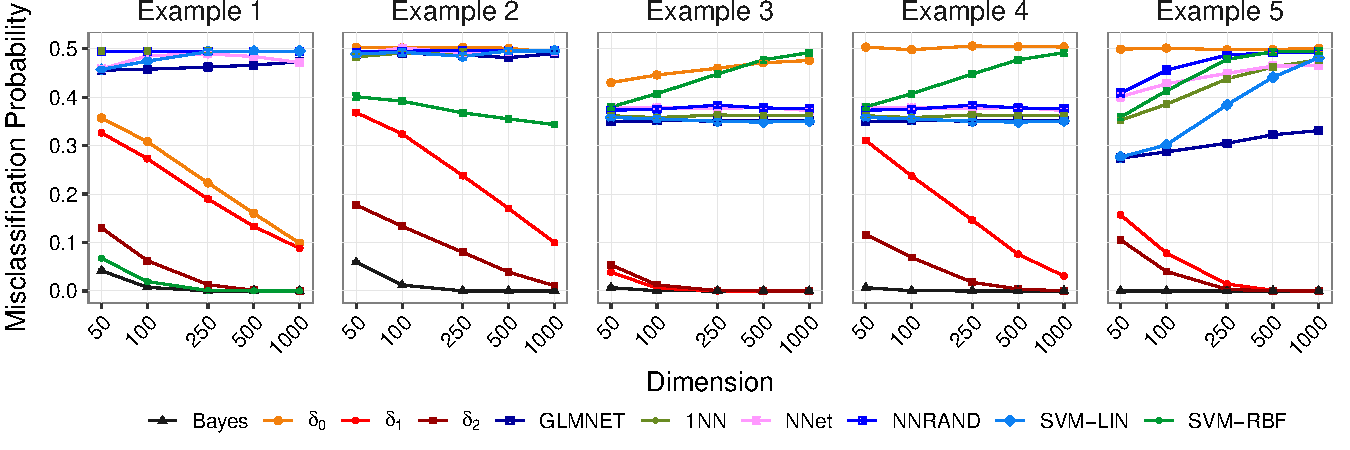
\includegraphics[width = \textwidth, height = 0.3\textwidth]{simu_plot_wide.pdf}
  %\vspace{0.05cm}
  \caption{Average Misclassification Rates (along with Standard Errors) Based on 100 Repetitions for Different Classifiers Are Plotted for Fixed $n\ (=40)$ and Increasing Values of $p$.}
  \label{completesim}
\end{figure*}
Suppose, A4 is satisfied for $\beta>0$, i.e., $p$ grows with $n$. One can prove that if assumptions A1 and A2 are satisfied, then ${\rm P}[|\bar{L}^0(\bZ)|< n^{-\gamma}]$ and ${\rm P}[|\bar{\theta}^0(\bZ)|< n^{-\gamma}]$ go to 0 as $\min\{n,p_n\}\to\infty$. Moreover, $\Delta^0_1$ and $\Delta^0_{2}$ decay to 0 under the same set of conditions. As a result, $\Delta_{j}\to 0\text{ as }\min\{n,p_n\}\to\infty\text{ for }j=1,2.$ The mathematical arguments for proving this convergence are quite similar to that of the proof of Theorem \ref{d1thm}.
\subsection{Computational Complexity}
Computing $\bar{T}_{jj^\prime}$ and $\bar{T}_j(\bz)$ for $\bz\in\mathbb{R}^p$ requires $O(n^2p)$ and $O(np)$ operations, respectively, for $j,j^\prime\in\{1,2\}$. Thus, the overall complexity of classifying an observation using $\delta_1$ and $\delta_2$ is $O(n^2p)$. Clearly, the complexity scales linearly with $p$. This makes the methods advantageous when the classification problem is particularly high-dimensional. The average time taken by these classifiers to classify a test observation is reported in Table \ref{order.d1.d2} of Supplementary \ref{supB}. %It clearly shows the advantage of using $\delta_1$ and $\delta_2$ over some popular classifiers.
\begin{comment}

\begin{tcolorbox}[colback=white]
Computing $\bar{T}_{jj^\prime}$ and $\bar{T}_j(\bz),\ \bz\in\mathbb{R}^p$ require $O(n^2p)$ and $O(np)$ operations, respectively, for $j,j^\prime\in\{1,\ldots, J\}$. Overall complexity is $O(n^2p)$. It increases linearly with respect to $p$ and makes the methods advantageous in analyzing high-dimensional data sets.
\end{tcolorbox}
\end{comment}
%Recall that $\log p_n \leq $Note that $\{n^{1-2\alpha_1}-n^\beta, n\geq 1\}$ is an increasing sequence since $\alpha_1<(1-\beta)/2$ (due to A3). Therefore, $\exp\{-B_2\{n^{1-2\alpha_1}-n^\beta\}\}=o(1)$ and consequently, under absolute continuity of $\bF_1$ and $\bF_2,$ Theorem \ref{d1thmUH} suggests that $\Delta_1-\Delta^0_1$ converges to 0 as $n\to\infty.$

%A5. There exist $0<\alpha_2<(1-\beta)/4$ such that $1/\bar{\tau}_{p_n}=o(n^{\alpha_2})$.

%Again, since $1-4\alpha_2>\beta$ due to A5, $\{n^{1-4\alpha_2}-n^\beta,n\geq 1\}$ is an increasing sequence and subsequently, $\exp\{-B_3\{n^{1-4\alpha_2}-n^\beta\}\}=o(1)$.
\begin{comment}
 \begin{tcolorbox}[colback=white]
  \textcolor{red}{Misclassfication probabilities converge to 0 even if the dimension grows faster than a polynomial of any degree of $n$.}\newline

  \noindent \textcolor{red}{Decaying rate of the misclassfication probabilities are exponential in $n$.}
\end{tcolorbox}
\end{comment}

% but under sub-gaussianity of random variables.% , i.e., A4 abd A5 are satisfied. Then the classifiers can still achieve {\it perfect classification} due to Theorem \ref{d1thmUH} and \ref{d2thmUH}.
\section{SIMULATION STUDY}\label{sim}
In this section, we analyze some simulated data sets to compare the classifiers $\delta_0,\delta_1$ and $\delta_2$ with some popular classifiers like GLMNET \citep{hastie2009elements}, the usual 1NN, NN based on the random projection method (NN-RAND) \citep{deegalla2006reducing}, neural networks (NNET) \citep{bishop1995neural}, SVM-LIN and SVM-RBF. All numerical exercises are performed on an Intel Xeon Gold 6140 CPU (2.30GHz, 2295 Mhz) using the  statistical software {\tt R}. Details about the packages used and parameters related to implementation of the popular classifiers are provided in Supplementary \ref{supB}.

Recall {\bf Examples \ref{ex1}} and {\bf \ref{ex2}} introduced in Section \ref{intro}. Three more examples are considered to compare the performances of these classifiers.
\vspace{-0.15cm}
\begin{ex}\label{ex3}
 $X_{1k}\stackrel{i.i.d.}{\sim} C(0,1)$ and $Y_{1k}\stackrel{i.i.d.}{\sim} C(1,1)$,
\end{ex}
\vspace{-0.15cm}
\begin{ex}\label{ex4}
$X_{1k}\stackrel{i.i.d.}{\sim} C(0,1)$ and $Y_{1k}\stackrel{i.i.d.}{\sim} C(0,2)$,
\end{ex}
\vspace{-0.15cm}
\begin{ex}\label{ex5}
 $X_{1k}$ $\stackrel{i.i.d.}{\sim}$ ${\rm Par}(1,1)$ and $Y_{1k}\stackrel{i.i.d.}{\sim}{\rm Par}(1.25,1)$,
\end{ex}
\vspace{-0.15cm}
for $1\le k\le p$. Here, $C(\mu,\sigma)$ denotes the Cauchy distribution with location $\mu\in\mathbb{R}$ and scale $\sigma>0$, while ${\rm Par}(\theta,s)$ denotes the Pareto distribution with $\theta>0$ and scale $s>0$.

{\bf Examples \ref{ex3}}, {\bf \ref{ex4}} and {\bf \ref{ex5}} correspond to a location, scale and  location-scale problem, respectively. All three examples involve heavy-tailed distributions. %$\bF_1$ and $\bF_2$ in Examples 1-4 are symmetric about $\0$, while in Example 5 they are positively-skewed.
In each example, we simulated data for $p=50$, $100$, $250$, $500$ and $1000$. The training sample was formed with $20$ observations from each class and a test set of size $200$ ($100$ from each class) was used. This process was repeated $100$ times to estimate the misclassification probabilities, which are reported in Table \ref{simtab} of Supplementary \ref{supA} along with their standard errors.

The performance of $\delta_0$ in {\bf Examples 1} and {\bf 2} was already discussed in Section \ref{method}. %The misclassification probability of $\delta_0$ decreases in this example as dimension increases. However, in {\bf Examples 2}-{\bf 5}, the performance of $\delta_0$ is quite poor as it misclassifies 50\% of the test observations. Recall Theorem \ref{theorem0} and note that the condition (b) is satisfied in {\bf Example 1} since $\nu_{11}=\nu_{12}=\nu_{22}=1$ and $|\sigma^2_1-\sigma^2_2|=1.$ Also, assumptions {\rm (i)-(iii)} are satisfied, and the theorem holds. On the other hand, $\nu_{11}=\nu_{12}=\nu_{22}=0$ and $|\sigma^2_1-\sigma^2_2|=0$ in {\bf Example 2}, violating both (a) and (b). Thus, Theorem \ref{theorem0} does not hold and $\delta_0$ fails.
Figure \ref{completesim} shows that $\delta_0$ fails miserably in {\bf Examples 3}-{\bf 5}. Observe that assumption (iii) is violated for these examples since the competing distributions are heavy-tailed. Consequently, Theorem \ref{theorem0} fails to hold and we observe poor performance of $\delta_0$ in these examples.

\noindent The classifiers $\delta_1$ and $\delta_2$ lead to promising results in all examples. Assumption A1 is satisfied in these examples since the component variables are independently distributed. Also, the marginals are identical, i.e., $F_{1,k}=F_{1,1}$ and $F_{2,k}=F_{2,1}$ for all $1\le k\le p.$ Thus, $\bar{\tau}_p\ (=\tau_1>0)$ is free of $p$. Hence, A2 is satisfied and Theorem \ref{d1thm} holds for all the examples. % both $n$ and

Figure \ref{completesim} shows that the misclassification probability of $\delta_2$ is smaller than that of $\delta_1$ in {\bf Examples 1}, {\bf 2}, {\bf 4} and {\bf 5}. Whereas, $\delta_1$ outperformed $\delta_2$ in {\bf Example 3}. Recall that the relative performance of these classifiers is goverened by the ordering among $\bar{T}_{11},\ \bar{T}_{12},$ and $\bar{T}_{22}$ (see the discussion in Section \ref{d1vsd2}). %Following Theorem \ref{cmpr_d1_d2}, we estimated $\bar{\tau}_p(1,1),\ \bar{\tau}_p(1,2),$ and $\bar{\tau}_p(2,2)$ by $\bar{T}_{11},\ \bar{T}_{12},$ and $\bar{T}_{22},$ respectively, for all examples and found that
We observed that $\bar{T}_{12}< \min\{\bar{T}_{11},\bar{T}_{22}\}$ in {\bf Example 3} while $\bar{T}_{12}> \min\{\bar{T}_{11},\bar{T}_{22}\}$ in the other examples (see Table \ref{order.d1.d2} of Supplementary \ref{supB}). These numerical findings are consistent with our claim in Theorem \ref{cmpr_d1_d2}.

In general, all the popular classifiers exhibited poor performance (except for a few instances). In {\bf Example 1}, only SVM-RBF identified the difference between scales of the competing populations and yielded {\it perfect classification}. The rest of the methods failed miserably and misclassified nearly 50\% of the test observations. In {\bf Example 2}, none of the classifiers had satisfactory results since in HDLSS settings, they are unable to discriminate between populations with same location and scale. In {\bf Examples 3}-{\bf 5}, the competing distributions are heavy-tailed and we observe deteriorating performances of all the popular classifiers.

\section{REAL DATA ANALYSIS}\label{real}
We study the performance of the proposed classifiers in two real data sets, namely, {\tt Computers} and  {\tt SmoothSubspace} available at the UCR Time Series Archive \citep[see][]{UCRArchive2018}. These data sets have {\it fixed training} and {\it test sets}. For our analysis, we combined the training and test data. We randomly selected $50\%$ of the observations from the combined set to form a new set of training observations, while keeping the proportions of observations from different classes consistent. The remaining observations were considered as the test set. This procedure was repeated $100$ times to obtain stable estimates of the misclassification probabilities. %over different splits of the data set

\noindent The {\tt Computers} (say, {\tt Comp}) data contains readings on electricity consumption from households in UK, sampled in two-minute intervals over a month. Each observation is of length 720 making the data high-dimensional. Classes are `Desktop' and `Laptop' with 250 (125 training and 125 test) samples in each. From Table \ref{realtab}, we observe that $\delta_0$ performed quite poorly, misclassifying almost half of the test observations. The mislassification probability of $\delta_2$ is smaller than that of $\delta_1$ in this data. To understand the relative performance of the classifiers $\delta_1$ and $\delta_2,$ we computed $\bar{T}_{11}=0.972$, $\bar{T}_{12}=1.043$, and $\bar{T}_{22}=1.155.$ Observe that $\bar{T}_{12}$ lies in between $\bar{T}_{11}$ and $\bar{T}_{22}$. As discussed in Section \ref{d1vsd2}, this relationship among $\bar{T}_{11},\bar{T}_{12}$ and $\bar{T}_{22}$ explains the superior performance of $\delta_2$ over $\delta_1.$ In fact, $\delta_2$ outperformed all the classifiers. The regularized classifier GLMNET secured the third position with a competitive performance. It was closely followed by SVM-RBF, whereas 1NN, NNRAND, NNET and SVM-LIN misclassified more than 40\% of the observations.

\noindent The second data set {\tt SmoothSubspace} (say, {\tt SSub}) is about testing the ability of a clustering algorithm to extract smooth subspaces for clustering time series data. This data set has 3 classes with 100 (50 train and 50 test) observations each. The observations have dimension 15. We observe in Table \ref{realtab} that the classifier $\delta_0$ misclassified more than 18\% of the test observations. It also perfromed the worst among all the classifiers. $\delta_1$ yielded the lowest misclassfication rate, while $\delta_2$ had the second best performance. We computed $\bar{T}_{11}=1.384$, $\bar{T}_{22}=1.378$, $\bar{T}_{33}=1.386$, $\bar{T}_{12}=1.340$, $\bar{T}_{13}=1.326$, and $\bar{T}_{23}=1.314$. Observe that $\bar{T}_{jj^\prime}<\min\{\bar{T}_{jj},\bar{T}_{j^\prime j^\prime}\}$ for all $ j\neq j^\prime $. These inequalities justify why the classifier $\delta_1$ outperformed $\delta_2$ in this data set.
%i.e., both $\bar{T}_{jj} - \bar{T}_{jj^\prime}$ and $\bar{T}_{j^\prime j^\prime}-\bar{T}_{j j}$ are positive for all $1\leq j\neq j^\prime \leq 3$.Thus, squaring the differences to amplify the measure of separation between $\bF_j$ and $\bF_{j^\prime}$ becomes unneccessary for all $j\neq j^\prime$.
Among the existing methods, NNET had the worst classfication accuracy. The linear classifiers GLMNET and SVM-LIN also performed very poorly, while non-linear classifiers like 1NN, NNRAND and SVM-RBF yielded improved misclassfication rates. In particular, SVM-RBF yielded the lowest misclassification rate among the popular classifiers, closely followed by NN-RAND. However, their misclassification probabilities are six times worse than that of $\delta_1$.
\begin{table}[h]%[9]{l}{\linewidth}
\scriptsize
\caption{\small Average Misclassification Rates of Classifiers (in \%)  with Standard Errors in Parentheses}
\label{realtab}
\setlength{\tabcolsep}{1pt} % Default value:    6pt
\vspace{3pt}
\begin{tabular}{ccccccccccccc}
\hline
Data  & $\delta_0$ & $\delta_1$ & $\delta_2$ & GLM & 1NN   & NN    & NNet  & SVM & SVM \\
&&&&NET&&RAND&&LIN&RBF\\ \hline %\{$J$, $p$, $n$\}
{\tt Comp}   & 47.09      & 36.40           & {\bf 35.47}           & 39.10  & 42.67 & 42.04 & 46.80 & 46.16  & 39.95  \\
            $J=2$ & (0.24)       & (0.22)            & (0.21)  & (0.24)   & (0.28)  & (0.27)  & (0.28)  & (0.34)   & (0.27)   \\ %\hline \{2, 750, 250\}
{\tt SSub} &  18.15      & {\bf 1.05}            & 1.33            & 13.35  & 8.71  & 7.09  & 16.19 & 10.79  & 6.35   \\
          $J=3$ & (0.27)       & (0.06)            & (0.08)            & (0.28)   & (0.20)  & (0.22)  & (0.44)  & (0.28)   & (0.19)   \\ \hline %\{3, 15, 150\}
\end{tabular}
\vspace{-0.1in}
\end{table}%\vspace{-0.1in}

\section{CONCLUDING REMARKS}\label{conclude}
In this article, we have developed some classifiers that utilize the difference between one-dimensional marginals of the underlying distributions to classify new data points. We have proved that the misclassification probability of these classifiers go to zero (i.e., {\it perfect classification}) in the HDLSS asymptotic regime under very general conditions. The proposed classifiers also have strong theoretical properties in  \emph{ultrahigh-dimensional} settings. They yield {\it perfect classification} even when the competing distributions are heavy-tailed. Furthermore, the proposed methods are free from tuning parameters. Using several simulated and real data sets, we have demonstrated promising performance of our classifiers.

%\noindent 
Suppose that the underlying distributions have identical one-dimensional marginals, and discriminatory information comes from joint distributions of the components. Under such circumstances, discriminants of the proposed classifiers need to be modified in a way such that they capture this difference between joint distributions (see \cite{roy2022generalizations}). 
%This requires further modification of the proposed classifiers.
%theoretical analysis which is out of scope of this article.  %A recent work by \cite{dedieu2019error} discusses error bounds of sparse classifiers in high dimensions.

Another aspect is handling the sparse signal setting. In our theoretical investigations, assumption A2 corresponds to the case when the number of components carrying discriminatory information scales as $p$. This assumption can be relaxed further. In particular, if the variables are weakly dependent, then Theorem \ref{d1thm} continues to hold if the number of informative components scales as $p^\alpha$ (for some $1/2<\alpha\le 1$). However, in practice, one whould be interested in capturing sparsity in a data dependent way and modify the classifier accordingly. This is a topic of future research. % (see \cite{SBG2020} for more details)

%\newpage %~\newpage
\acknowledgments

We thank the reviewers for their careful reading of an earlier version of the article and providing us with helpful comments. We would also like to thank Purushottam Kar and Soham Sarkar for their valuable inputs which improved this article.

\bibliography{citation}
% Supplementary material: To improve readability, you must use a single-column format for the supplementary material.

%%%%%%%%%%%%%%%%%%%%%%%%%%%%%%%%%%%
%%%%%% SUPPLEMENT  %%%%%%
%%%%%%%%%%%%%%%%%%%%%%%%%%%%%%%%%%%

\clearpage
\appendix
\thispagestyle{empty}
\onecolumn
\makesupplementtitle
\section{MATHEMATICAL DETAILS AND PROOFS}\label{supA}
%\begin{tcolorbox}[colback = white]
We will use the following definitions in our proofs presented below.
\begin{enumerate}
 \item $a_n=o(b_n)$ as $n\to\infty$ implies that for every $\epsilon>0$ there exists an $N\in\mathbb{N}$ such that $|a_n/b_n|<\epsilon$ for all $n\geq N$.
 \item $a_n=O(b_n)$ as $n\to\infty$ implies that there exist $M>0$ and $N\in\mathbb{N}$ such that $|a_n/b_n|<M$ for all $n\geq N$.
\end{enumerate}
%\end{tcolorbox}
\vspace{0.5cm}
% \emph{Results up to Theorem \ref{cmpr_d1_d2} in HDLSS asymptotic regime are derived for a fixed $n$ and $p\to\infty$}.\newline
\begin{lemma}\label{C0}
Suppose $\bU\sim\bF_j$ and $\bV\sim\bF_{j^\prime}$ for $j,j^\prime\in\{1,2\}$ and $\bU,\bV$ are independent. If assumptions (i)-(iii) are satisfied, then $$\left |h(\bU,\bV)- \frac{1}{2\pi}\sin^{-1}\left (\frac{\nu_{jj^\prime}}{\big [(\sigma_j^2 + \nu_{jj})(\sigma_{j^\prime}^2 + \nu_{j^\prime j^\prime})\big ]^{\frac{1}{2}}}\right )\right |\stackrel{\rm P}{\to}0\text{ as }p\to\infty.$$
\end{lemma}

\noindent {\bf Proof of Lemma \ref{C0}}
We have assumed in (ii) that the limiting constants $\nu_{jj^\prime},$ and $\sigma^2_j$ exist for $j,j^\prime\in\{1,2\}.$ Fix $\epsilon>0$. Now, observe that
\begin{align*}
\ {\rm P}\bigg [\bigg |\frac{1}{p}\bU^\top\bV - \nu_{jj^\prime}\bigg |>\epsilon\bigg ]
=&\ {\rm P}\bigg [\bigg |\frac{1}{p}\bU^\top\bV - \frac{1}{p}\bmu_j^\top\bmu_{j^\prime} + \frac{1}{p}\bmu_j^\top\bmu_{j^\prime} - \nu_{jj^\prime}\bigg |>\epsilon\bigg ]\\
\leq &\ {\rm P}\bigg [\bigg |\frac{1}{p}\bU^\top\bV - \frac{1}{p}\bmu_j^\top\bmu_{j^\prime}\bigg |>\frac{\epsilon}{2}\bigg ] + {\rm I}\bigg [\bigg |\frac{1}{p}\bmu_j^\top\bmu_{j^\prime} - \nu_{jj^\prime}\bigg |>\frac{\epsilon}{2}\bigg ]\ [\text{using the union bound}].
\end{align*}
Since $\lim_{p\to\infty}\bmu_j^\top\bmu_{j^\prime}=\nu_{jj^\prime}$, there exists $p_0\in\mathbb{N}$ such that ${\rm I}\left [\left |\frac{1}{p}\bmu_j^\top\bmu_{j^\prime} - \nu_{jj^\prime}\right |>\frac{\epsilon}{2}\right ]=0$ for all $p\geq p_0$. So, we get $${\rm P}\bigg [\bigg |\frac{1}{p}\bU^\top\bV - \nu_{jj^\prime}\bigg |>\epsilon\bigg ]\leq {\rm P}\bigg [\bigg |\frac{1}{p}\bU^\top\bV - \frac{1}{p}\bmu_j^\top\bmu_{j^\prime}\bigg |>\frac{\epsilon}{2}\bigg ]\text{ for all }p\ge p_0.$$
Observe that
\begin{align}\label{ref1}
&\ {\rm P}\bigg [\bigg |\frac{1}{p}\bU^\top\bV - \frac{1}{p}\bmu_j^\top\bmu_{j^\prime}\bigg |>\frac{\epsilon}{2}\bigg ]\\
= &\ {\rm P}\left [\bigg |\frac{1}{p}\sum_{k=1}^p U_{k}V_k - \frac{1}{p}\sum_{k=1}^p {\rm E}[ U_{k}]{\rm E}[V_k]\bigg |>\frac{\epsilon}{2}\right]\nonumber\\
\leq &\ \frac{4}{\epsilon^2}{\rm Var}\bigg [\frac{1}{p}\sum_{k=1}^p U_{k}V_{k}\bigg ]\ [\text{using Chebyshev's inequality}]\nonumber \\
=&\ \frac{4}{\epsilon^2 p^2}\sum_{k=1}^p {\rm Var}\big [U_{k}V_{k})\big ]
 +\frac{8}{\epsilon^2 p^2}\mathop{\sum\sum}_{1\leq k< k^\prime\leq p} {\rm Cov}\left(U_{k}V_{k},U_{k^\prime}V_{k^\prime}\right)\nonumber \\
\leq &\ \frac{4}{\epsilon^2 p^2}\sum_{k=1}^p {\rm E}\big [U^2_{k}V^2_{k})\big ]
 +\frac{8}{\epsilon^2 p^2}\mathop{\sum\sum}_{1\leq k< k^\prime\leq p} {\rm Corr}\left(U_{k}V_{k},U_{k^\prime}V_{k^\prime}\right)\sqrt{{\rm E}\big [U^2_{k}V^2_{k})\big ]\ {\rm E}\big [U^2_{k^\prime}V^2_{k^\prime})\big ]}\nonumber \\
 \leq &\ \frac{4C}{\epsilon^2 p}
 +\frac{8C}{\epsilon^2 p^2}\mathop{\sum\sum}_{1\leq k< k^\prime\leq p} {\rm Corr}\left(U_{k}V_{k},U_{k^\prime}V_{k^\prime}\right)\ [\text{for some }C<\infty\ (\text{due to (i)})]\nonumber \\
 =&\ o(1)\text{ as }p\to\infty\ [\text{using (iii)}].
\end{align}
Therefore, ${\rm P}\left [\left |\frac{1}{p}\bU^\top\bV - \nu_{jj^\prime}\right |>\epsilon\right ]\leq {\rm P}\left [\left |\frac{1}{p}\bU^\top\bV - \frac{1}{p}\bmu_j^\top\bmu_{j^\prime}\right |>\frac{\epsilon}{2}\right ] =o(1)$ for $\bU\sim\bF_j$ and $\bV\sim\bF_{j^\prime}$ with $j,j^\prime\in\{1,2\}$ as $p\to\infty$.

Following similar arguments, one can also prove that (as $p\to\infty$),
\begin{align*}
&\ {\rm P}\left [\left |\frac{1}{p}\|\bU\|^2 - \frac{1}{p}{\rm E}[\|\bU\|^2]\right |>\epsilon\right ]\leq o(1)\\
\Rightarrow &\ {\rm P}\left [\left |\frac{1}{p}\|\bU\|^2 - \frac{1}{p}\left \{\|\bmu_i\|^2 + tr (\Sigma_j)\right \}\right |>\epsilon\right ]\leq o(1)\\
\Rightarrow &\ {\rm P}\left [\left |\frac{1}{p}\|\bU\|^2 - \left \{\nu_{jj} + \sigma^2_j\right \}\right |>\epsilon\right ]\leq o(1)\ [\lim_{p\to\infty}\|\bmu_j\|^2/p=\nu_{jj}\text{ and }\lim_{p\to\infty}tr (\Sigma_j)/p=\sigma^2_j].
\end{align*}
Using the continuous mapping theorem (repeatedly), we obtain
$$\sin (2\pi h(\bU,\bV))=\frac{1+\bU^\top\bV}{\sqrt{(1+\|\bU\|^2)(1+\|\bV\|^2)}}=\frac{\frac{1}{p}+\frac{\bU^\top\bV}{p}}{\sqrt{\left (\frac{1}{p}+\frac{\|\bU\|^2}{p}\right )\left(\frac{1}{p}+\frac{\|\bV\|^2}{p}\right)}}\stackrel{\rm P}{\to}\frac{\nu_{jj^\prime}}{\sqrt{(\sigma^2_j+\nu_{jj})(\sigma^2_{j^\prime}+\nu_{j^\prime j^\prime})}}$$ as $p\to\infty$. Consequently, we have $h(\bU,\bV)\stackrel{\rm P}{\to}\frac{1}{2\pi}\sin^{-1}\left \{\frac{\nu_{jj^\prime}}{\sqrt{(\sigma^2_j+\nu_{jj})(\sigma^2_{j^\prime}+\nu_{j^\prime j^\prime})}}\right\}$ as $p\to\infty$.

Hence, the proof. \hfill\QEDB\newline

Define $\tau_{ii}=\frac{1}{2\pi}\sin^{-1}\left \{\frac{\nu_{ii}}{(\sigma^2_i + \nu_{ii})}\right\}$ for $i=1,2$ and $\tau_{12}=\frac{1}{2\pi}\sin^{-1}\left \{\frac{\nu_{12}}{\sqrt{(\sigma^2_1 + \nu_{11})(\sigma^2_2 + \nu_{22})}}\right\}$. Lemma \ref{tau0def} suggests that $h(\bU,\bV)\stackrel{\rm P}{\to}\tau_{jj^\prime}$ as $p\to\infty$, where $\bU\sim\bF_j$, $\bV\sim\bF_{j^\prime}$ for $j,j^\prime\in\{1,2\}$ and $\bU,\bV$ are independent.
\begin{cor}\label{L0}
 For $j,j^\prime\in\{1,2\}$, if assumptions {\rm (i)-(iii)} are satisfied, then
 \begin{enumerate}[(a)]
  \item $|T_{jj^\prime}-\tau_{jj^\prime}|\stackrel{\rm P}{\to}0$ as $p\to\infty $, and
  \item if $\bZ\sim \bF_{j^\prime}$, then $|T_{j}(\bZ)-\tau_{jj^\prime}|\stackrel{\rm P}{\to}0$ as $p\to\infty $.
 \end{enumerate}
\end{cor}
\noindent {\bf Proof of Corollary \ref{L0}}
\begin{enumerate}[(a)]
 \item Fix $\epsilon>0$. It follows from Lemma \ref{tau0def} that
\begin{align}\label{ref1}
{\rm P}\big [\big |T_{11} - \tau_{11}\big |>\epsilon\big ]
= &\ {\rm P} \bigg [\bigg |\frac{1}{n_1(n_1-1)}\mathop{\sum\sum}\limits_{1\leq i\neq j\leq n_1}\left\{{h}(\bX_{i},\bX_{j})-\tau_{11}\right\}\bigg |>\epsilon \bigg]\nonumber\\
\leq &\ {\rm P} \bigg [\frac{1}{n_1(n_1-1)}\mathop{\sum\sum}\limits_{1\leq i\neq j\leq n_1}\left |{h}(\bX_{i},\bX_{j}) -\tau_{11}\right |>\epsilon \bigg]\nonumber \\
\leq &\ \mathop{\sum\sum}\limits_{1\leq i\neq j\leq n_1}{\rm P} \left [\left |{h}(\bX_{i},\bX_{j}) -\tau_{11}\right |>\epsilon \right]\nonumber\\
=&\ n_1(n_1-1)o(1)=\ o(1)\text{ as }p\to\infty\ [\text{$n_1$ is fixed}].
\end{align}
Therefore, $|T_{11}-\tau_{11}|\stackrel{\rm P}{\to}0$ as $p\to\infty$. Similarly, $|T_{12}-\tau_{12}|$ and $|T_{22}-\tau_{22}|$ also converge in probability to 0 as $p\to\infty$.
\item Fix $\epsilon>0$. Let $\bU\in\rchi_i$ (i.e., $\bU\sim\bF_j$) and $\bZ\sim\bF_{j^\prime}$ for $j,j^\prime\in\{1,2\}$. Since $n_j$ is fixed for $j\in\{1,2\}$, using Lemma \ref{tau0def}, we have
\begin{align}\label{ref3}
{\rm P}\big [\big |T_{j}(\bZ) - \tau_{jj^\prime}\big |>\epsilon\mid\bZ\sim\bF_{j^\prime}\big ]
=&\  {\rm P}\left [\left |\left \{\frac{1}{n_j}\sum_{\bU\in\rchi_j}\big \{h(\bU,\bZ) - {\rm E}[h(\bU,\bZ)\mid\bZ\sim\bF_{j^\prime}]\big \}\right \}\right |>\epsilon\bigg |\bZ\sim\bF_{j^\prime} \right ]\nonumber\\
\leq &\ {\rm P}\left [\frac{1}{n_j}\sum_{\bU\in\rchi_j}\left |h(\bU,\bZ) - {\rm E}[h(\bU,\bZ)\mid\bZ\sim\bF_{j^\prime}]\right |>\epsilon \bigg |\bZ\sim\bF_{j^\prime}\right ]\nonumber \\
\leq &\ \sum_{\bU\in\rchi_j}{\rm P}\left [\left |h(\bU,\bZ) - {\rm E}[h(\bU,\bZ)\mid\bZ\sim\bF_{j^\prime}]\right |>\epsilon \mid\bZ\sim\bF_{j^\prime}\right ]\nonumber \\
\leq &\ n_jo(1)=o(1)\text{ as }p\to\infty\ [ n_j\text{ is fixed].}
\end{align}
\end{enumerate}
Hence, the proof. \hfill \QEDB\newline

Recall the definition of $\tau_0$ given as follows:
\begin{align*}
 &\ \tau_0 = \frac{1}{2\pi}\sin^{-1}\left \{\frac{\nu_{11}}{(\sigma^2_1 + \nu_{11})}\right\}+ \frac{1}{2\pi}\sin^{-1}\left \{\frac{\nu_{22}}{(\sigma^2_2 + \nu_{22})}\right\}- \frac{1}{\pi}\sin^{-1}\left \{\frac{\nu_{12}}{\sqrt{(\sigma^2_1 + \nu_{11})(\sigma^2_2 + \nu_{22})}}\right\}\\
 \text{i.e., }&\ \tau_0=\tau_{11}+\tau_{22}-2\tau_{12}.
\end{align*}
If $\nu_{11}=\nu_{12}=\nu_{22}=0$, then $\tau_0=0$. Also, if $\nu_{11}=\nu_{12}=\nu_{22}$ and $\sigma^2_1=\sigma^2_2$, then $\tau_0=0$.
\begin{comment}
 \begin{cor}\label{C0}
 Suppose assumptions {\rm (i)-(iii)} are satisfied. Let $\bZ$ be a test observation.
%  \vspace{-0.1cm}
%\begin{small}
\begin{enumerate}[(a)]
\item  $\begin{aligned}[t]&\text{If }\bZ\sim\bF_1,\text{ then }
|L_2(\bZ)- L_1(\bZ) - \tau_0|\stackrel{\rm P}{\to}0\text{ as } p\to\infty .
 \end{aligned}$
%\end{small}
%\vspace{-0.15cm}
\item  $\begin{aligned}[t]&\text{If }\bZ\sim\bF_2,\text{ then }
 |L_2(\bZ)- L_1(\bZ) + \tau_0|\stackrel{\rm P}{\to}0\text{ as } p\to\infty.
 \end{aligned}$
\end{enumerate}
\end{cor}
\end{comment}

\noindent {\bf Proof of Lemma \ref{tau0def}}
\begin{enumerate}[(a)]
 \item First of all, we have $|L(\bz)-\tau|\leq |L(\bz)-\tau_0|+|\tau-\tau_0|$ using triangle inequality for all $\bz\in\mathbb{R}^p.$

 Now, observe that $L(\bZ) = L_2(\bZ)- L_1(\bZ)= \{T_{22}-2T_2(\bZ)\}- \{T_{11} - 2T_1(\bZ)\}.$ If $\bZ\sim\bF_1$, then it follows from Corollary \ref{L0} that $$L(\bZ)\stackrel{\rm P}{\to}\{\tau_{22} - 2 \tau_{12}\} -\{ \tau_{11}-2\tau_{11}\}=\tau_{11}  + \tau_{22}- 2 \tau_{12}=\tau_0 \text{ as }p\to\infty.$$

 It follows from Lemma \ref{C0} that $h(\bX_1,\bX_2)\stackrel{\rm P}{\to}\tau_{11},h(\bX_1,\bY_1)\stackrel{\rm P}{\to}\tau_{12}$ and $h(\bY_1,\bY_2)\stackrel{\rm P}{\to}\tau_{22}$ as $p\to\infty.$ Since, $h$ is a bounded function, using the Dominated Convergence Theorem, we have  ${\rm E}[h(\bX_1,\bX_2)]\to\tau_{11},{\rm E}[h(\bX_1,\bY_1)]\to\tau_{12}$ and ${\rm E}[h(\bY_1,\bY_2)]\to\tau_{22}$ as $p\to\infty.$ Therefore, $\tau = {\rm E}[h(\bX_1,\bX_2)] + {\rm E}[h(\bX_1,\bX_2)] -2{\rm E}[h(\bX_1,\bX_2)]\to \tau_{11}+\tau_{22}-2\tau_{12}=\tau_0$ as $p\to\infty.$ Thus, $|L(\bZ)-\tau|\stackrel{\rm P}{\to}0$ as $p\to\infty.$
 \item The arguments for the proof of this part are similar to part (a), and we skip it.
\end{enumerate}
Hence, the proof. \hfill\QEDB\newline

\noindent {\bf Proof of Theorem \ref{theorem0}}

Recall that the prior probability of an observation $\bZ$ belonging to the $j$-th class is given by $\pi_j$ for $j=1,2$ with $\pi_1+\pi_2=1$. The misclassification probability of $\delta_0$ is as follows:
\begin{align}\label{ref501}
{\rm P}[\delta_0(\bZ)\neq \text{ true label of }\bZ]
 =&\ \pi_1 {\rm P}[\delta_0(\bZ)=2\mid \bZ\sim\bF_1] + \pi_2{\rm P}[\delta_0(\bZ)=1\mid \bZ\sim\bF_2]\nonumber \\
 =&\ \pi_1 {\rm P}[L_2(\bZ)\leq L_1(\bZ)\mid \bZ\sim\bF_1]+ \pi_2{\rm P}[L_2(\bZ)> L_1(\bZ)\mid \bZ\sim\bF_2].
\end{align}
We have assumed that either $(a)\ \nu_{11},\nu_{12},\nu_{22}$ are unequal, or $(b)\ \nu_{11}=\nu_{12}=\nu_{22}\neq 0$, and $\sigma_1^2=\sigma_2^2$ holds. As a consequence, $\tau_0$ is strictly positive. Fix $0<\epsilon<\tau_0$. Now, we have
\begin{align}\label{ref502}
{\rm P}\big [L_2(\bZ)\leq L_1(\bZ)\mid \bZ\sim\bF_1\big ]
&\ \leq {\rm P}\big [L_2(\bZ)- L_1(\bZ)\leq \tau_0-\epsilon\mid \bZ\sim\bF_1\big ]\nonumber \\
&\ \leq {\rm P}\big [L_2(\bZ)- L_1(\bZ)- \tau_0 \leq -\epsilon\mid \bZ\sim\bF_1\big ]\nonumber \\
&\ \leq {\rm P}\big [|L_2(\bZ)- L_1(\bZ) - \tau_0|>\epsilon\mid \bZ\sim\bF_1\big ]\nonumber\\
&\ =o(1)\text{ as }p\to\infty\ [\text{using Corollary \ref{C0}}(a)].
\end{align}
Similarly,
\begin{align}\label{ref503}
{\rm P}\big [L_2(\bZ)> L_1(\bZ)\mid \bZ\sim\bF_2\big ]
\leq &\ {\rm P}\big [L_2(\bZ)- L_1(\bZ)> -\tau_0+\epsilon\mid \bZ\sim\bF_2\big ]\nonumber \\
\leq &\ {\rm P}\big [L_2(\bZ)- L_1(\bZ)+ \tau_0 > \epsilon\mid \bZ\sim\bF_2\big ]\nonumber \\
\leq &\ {\rm P}\big [|L_2(\bZ)- L_1(\bZ) + \tau_0|>\epsilon\mid \bZ\sim\bF_2\big ]\nonumber\\
=&\ o(1)\text{ as }p\to\infty\ [\text{using Corollary \ref{C0}}(b)].
\end{align}
Combining  \eqref{ref501}, \eqref{ref502} and \eqref{ref503}, we get ${\rm P}[\delta_0(\bZ)\neq \text{ true label of }\bZ]=o(1)$ as $p\to\infty$.\hfill\QEDB\newline

\begin{lemma}\label{L.2}
  For $j,j^\prime\in\{1,2\}$, if {\rm A1} is satisfied, then
 \begin{enumerate}[(a)]
  \item $|\bar{T}_{jj^\prime}-\bar{\tau}_p(j,j^\prime)|\stackrel{\rm P}{\to}0$ as $p\to\infty $, and
  \item if $\bZ\sim \bF_j$, then $|\bar{T}_{j^\prime}(\bZ)-\bar{\tau}_p(j,j^\prime)|\stackrel{\rm P}{\to}0$ as $p\to\infty $.
 \end{enumerate}
\end{lemma}
\noindent {\bf Proof of Lemma \ref{L.2}}
\begin{enumerate}[(a)]
 \item Recall the definitions of $\bar{T}_{11}$ and $\bar{\tau}_p(1,1)$ given in \eqref{barLdef} and \eqref{estexpect}, respectively. Fix $\epsilon>0$. We have
\begin{align}\label{ref1}
&\ {\rm P}\big [\big |\bar{T}_{11} - \bar{\tau}_p(1,1)\big |>\epsilon\big ]\nonumber\\
= &\ {\rm P} \bigg [\bigg |\frac{1}{n_1(n_1-1)}\mathop{\sum\sum}\limits_{1\leq i\neq j\leq n_1}\bar{h}_p(\bX_{i},\bX_{j})-{\rm E}\left [\bar{h}_p(\bX_{1},\bX_{2})\right ]\bigg |>\epsilon \bigg]\nonumber\\
= &\ {\rm P} \bigg [\bigg |\frac{1}{p}\sum_{k=1}^p \frac{1}{n_1(n_1-1)}\mathop{\sum\sum}\limits_{1\leq i\neq j\leq n_1}{h}(X_{ik},X_{jk})-\frac{1}{p}\sum_{k=1}^p {\rm E}\left [ h(X_{1k},X_{2k})\right ]\bigg |>\epsilon \bigg]\ [\text{using the definition of }\bar{h}_p]\nonumber\\
= &\ {\rm P} \bigg [\bigg |\frac{1}{n_1(n_1-1)}\mathop{\sum\sum}\limits_{1\leq i\neq j\leq n_1}\frac{1}{p}\sum_{k=1}^p {h}(X_{ik},X_{jk}) -\frac{1}{p}\sum_{k=1}^p {\rm E}\left [ h(X_{1k},X_{2k})\right ]\bigg |>\epsilon \bigg]\nonumber \\
\leq &\ {\rm P} \bigg [\frac{1}{n_1(n_1-1)}\mathop{\sum\sum}\limits_{1\leq i\neq j\leq n_1}\bigg |\frac{1}{p}\sum_{k=1}^p {h}(X_{ik},X_{jk}) -\frac{1}{p}\sum_{k=1}^p {\rm E}\left [ h(X_{1k},X_{2k})\right ]\bigg |>\epsilon \bigg]\ [\text{using  triangle inequality}]\nonumber \\
\leq &\ \mathop{\sum\sum}\limits_{1\leq i\neq j\leq n_1}{\rm P} \bigg [\bigg |\frac{1}{p}\sum_{k=1}^p \big \{{h}(X_{ik},X_{jk}) -{\rm E}\left [ h(X_{1k},X_{2k})\right ]\big \}\bigg |>\epsilon \bigg]\ [\text{using the union bound}]\nonumber \\
\leq &\ \mathop{\sum\sum}\limits_{1\leq i\neq j\leq n_1} \frac{1}{\epsilon^2}{\rm Var}\bigg [\frac{1}{p}\sum_{k=1}^p h(X_{ik},X_{jk})\bigg ]\ [\text{using Chebyshev's inequality}].
\end{align}
Now, we will show that ${\rm Var}\left [\sum_{k=1}^p h(X_{ik},X_{jk})/p\right ]$ converges to 0 for all $i\neq j$ as $p\to\infty.$

Fix $1\leq i,j\leq n_1$ with $i\neq j$. Observe that
\begin{align}\label{ref2}
\hspace{-0.5cm}{\rm Var}\bigg [\frac{1}{p}\sum_{k=1}^p h(X_{ik},X_{jk})\bigg ]
=\ \frac{1}{p^2}\sum_{k=1}^p {\rm Var}\big [h(X_{ik},X_{jk})\big ]
 +\frac{2}{p^2}\mathop{\sum\sum}_{1\leq k< k^\prime\leq p} {\rm Cov}\left(h(X_{ik},X_{jk}),h(X_{ik^\prime},X_{jk^\prime})\right).
\end{align}
Since $0\leq h\leq 1,$ we have $ {\rm Var}\big [h(X_{ik},X_{jk})\big ]\leq 1$ for all $1\le k\le p.$ Using the inequality ${\rm Cov}(X,Y)\leq {\rm Corr}(X,Y)\sqrt{{\rm E}(X^2){\rm E}(Y^2)}$ and the boundedness of $h$, we get
\begin{align*}
{\rm Cov}\left(h(X_{ik},X_{jk}),h(X_{ik^\prime},X_{jk^\prime})\right)\leq {\rm Corr}\left(h(X_{ik},X_{jk}),h(X_{ik^\prime},X_{jk^\prime})\right)\text{ for all }1\leq k<k^\prime\leq p.
\end{align*}
Since A1 is satisfied, from \eqref{ref2} we obtain
\begin{align*}
{\rm Var}\bigg [\frac{1}{p}\sum_{k=1}^p h(X_{ik},X_{jk})\bigg ]
\leq \frac{1}{p} +\frac{2}{p^2}\mathop{\sum\sum}_{1\leq k< k^\prime\leq p} {\rm Corr}\left(h(X_{ik},X_{jk}),h(X_{ik^\prime},X_{jk^\prime})\right)
= o(1)\text{ as }p\to\infty.
\end{align*}
It now follows from \eqref{ref1} that $|\bar{T}_{11}-\bar{\tau}_p(1,1)|\stackrel{\rm P}{\to}0$ as $p\to\infty.$ Following similar arguments, one can show that if A1 is satisfied, then both $|\bar{T}_{12}-\bar{\tau}_p(1,2)|$ and $|\bar{T}_{22}-\bar{\tau}_p(2,2)|$ converge in probability to 0 as $p\to\infty$.

\item Fix $\epsilon>0,$ and recall the definitions of $\bar{T}_{1}(\bZ)$ and $\bar{\tau}_p(1,1)$. We have
\begin{align}\label{ref3}
&\ {\rm P}\big [\big |\bar{T}_{1}(\bZ) - \bar{\tau}_p(1,1)\big |>\epsilon\mid \bZ\sim\bF_1\big ]\nonumber \\
= &\ {\rm P}\left [\bigg |\frac{1}{p}\sum_{k=1}^p T_{1k}(Z_k) - \frac{1}{p}\sum_{k=1}^p {\rm E}\left [ h(X_{1k},X_{2k})\right ]\bigg |>\epsilon\Big | \bZ\sim\bF_1 \right ]\nonumber \\
= &\ {\rm P}\bigg [\bigg |\frac{1}{p}\sum_{k=1}^p \frac{1}{n_1}\sum_{i=1}^{n_1}\big \{h(X_{ik},Z_k) - {\rm E}[h(X_{1k},Z_k)\mid \bZ\sim\bF_1]\big \}\bigg |>\epsilon\Big | \bZ\sim\bF_1 \bigg ]\nonumber \\
= &\ {\rm P}\bigg [\bigg |\frac{1}{n_1}\sum_{i=1}^{n_1}\frac{1}{p}\sum_{k=1}^p\big \{h(X_{ik},Z_k) - {\rm E}[h(X_{1k},Z_k)\mid \bZ\sim\bF_1]\big \}\bigg |>\epsilon\Big | \bZ\sim\bF_1 \bigg ]\nonumber \\
\leq &\ {\rm P}\bigg [\frac{1}{n_1}\sum_{i=1}^{n_1}\bigg |\frac{1}{p}\sum_{k=1}^p\big \{h(X_{ik},Z_k) - {\rm E}\left [h(X_{1k},Z_k)\mid \bZ\sim\bF_1\right ]\big \}\bigg |>\epsilon\Big | \bZ\sim\bF_1 \bigg ]\ [\text{using triangle inequality}]\nonumber \\
\leq &\ \sum_{i=1}^{n_1}{\rm P}\bigg [\bigg |\frac{1}{p}\sum_{k=1}^p\big \{h(X_{ik},Z_k) - {\rm E}\left [h(X_{1k},Z_k)\mid \bZ\sim\bF_1\right ]\big \}\bigg |>\epsilon\Big | \bZ\sim\bF_1 \bigg ]\ [\text{using the union bound}]\nonumber \\
\leq &\ \sum_{i=1}^{n_1}\frac{1}{\epsilon^2}{\rm Var}\bigg [\frac{1}{p}\sum_{k=1}^p h(X_{ik},Z_k)\Big | \bZ\sim \bF_1\bigg ]\ [\text{using Chebyshev's inequality}]\nonumber \\
=&\  \sum_{i=1}^{n_1}\frac{1}{\epsilon^2}{\rm Var}\bigg [\frac{1}{p}\sum_{k=1}^p h(X_{ik},X^\prime_k)\bigg ],
\end{align}
where $\bX^\prime=(X^\prime_1,\ldots, X^\prime_p)^\top\sim\bF_1$ and it is independent of $\rchi_1.$ Using the boundedness of $h$ and assumption A1, we have shown in part (a) of Lemma \ref{L2} that ${\rm Var}\big [\frac{1}{p}\sum_{k=1}^p h(X_{ik},X^\prime_k)\big ]=o(1)$ as $p\to\infty$. Since $n_1$ is fixed, $\sum_{i=1}^{n_1}{\rm Var}\big [\frac{1}{p}\sum_{k=1}^p h(X_{ik},X^\prime_k)\big ]=o(1)$ as $p\to\infty$. Therefore, it follows from \eqref{ref3} that $\big |\bar{T}_{1}(\bZ) - \bar{\tau}_p(1,1)\big |$ converges in probability to 0 as $p\to\infty$ (when $\bZ\sim\bF_1$).

Following similar arguments, one can prove that $
{\rm P}\big[\big |\bar{T}_{2}(\bZ) - \bar{\tau}_p(1,2)\big |>\epsilon\mid\bZ\sim\bF_1\big ],\ {\rm P}\big[\big |\bar{T}_{1}(\bZ) - \bar{\tau}_p(1,2)\big |>\epsilon\mid\bZ\sim\bF_2\big ]$ and ${\rm P}\big[\big |\bar{T}_{2}(\bZ) - \bar{\tau}_p(2,2)\big |>\epsilon\mid\bZ\sim\bF_2\big ]$ also converge to 0 as $p\to\infty.$
\end{enumerate}
Hence, the proof. \hfill \QEDB\newline

\noindent {\bf Proof of Lemma \ref{L2}}

Recall that $\bar{L}_1(\bZ) = \bar{T}_{11} - 2\bar{T}_{1}(\bZ),\ \tilde{L}_{2}(\bZ) = \bar{T}_{22} - 2\bar{T}_{2}(\bZ)$ and
\begin{align}\label{ref6}
 \bar{\theta}(\bZ) =&\ \frac{1}{2}\bar{T}(\bar{L}_2(\bZ)-\bar{L}_1(\bZ)) + \frac{1}{2}(\bar{T}_{22}-\bar{T}_{11})(\bar{L}_2(\bZ)+\bar{L}_1(\bZ)+2\bar{T}_{12})\nonumber \\
 =&\ \frac{1}{2}\big \{(\bar{T}_{11}-2\bar{T}_{12}+\bar{T}_{22})\times (\bar{L}_2(\bZ)-\bar{L}_1(\bZ))\big \}\nonumber \\
  +&\ \frac{1}{2}\big \{(\bar{T}_{22}-\bar{T}_{11})\times (\bar{T}_{22} - 2\bar{T}_2(\bZ) + \bar{T}_{11} - 2\bar{T}_1(\bZ)+2\bar{T}_{12})\big \}.
\end{align}
Let us denote $\bar{L}_2(\bZ)-\bar{L}_1(\bZ)$ by $\bar{L}(\bZ)$ and $\bar{T}_{22} - 2\bar{T}_2(\bZ) + \bar{T}_{11} - 2\bar{T}_1(\bZ)+2\bar{T}_{12}$ by $\bar{S}(\bZ)$.
\begin{align}\label{ref7}
\hspace{-1.75in}
\text{We can write }\bar{\theta}(\bZ) = \frac{1}{2}\big \{(\bar{T}_{11}-2\bar{T}_{12}+\bar{T}_{22})\times \bar{L}(\bZ)\big \}
 +\frac{1}{2}\big \{(\bar{T}_{22}-\bar{T}_{11})\times \bar{S}(\bZ)\big \}.
\end{align}
\begin{enumerate}[(a)]
 \item Fix $\epsilon >0.$ Now,
\begin{align}\label{ref4}
 &\ {\rm P}\big [|\bar{L}(\bZ) - \bar{\tau}_p|>\epsilon\mid \bZ\sim\bF_1\big ]= {\rm P}\big [|\bar{L}_2(\bZ)- \bar{L}_1(\bZ) - \bar{\tau}_p|>\epsilon\mid \bZ\sim\bF_1\big ]\nonumber \\
 =&\ {\rm P}\big [|\{\bar{T}_{22} - 2\bar{T}_2(\bZ)- \bar{T}_{11} + 2\bar{T}_1(\bZ)\}
 - \{\bar{\tau}_p(1,1) - 2\bar{\tau}_p(1,2) +\bar{\tau}_p(2,2)\}|>\epsilon\mid \bZ\sim\bF_1\big ]\nonumber \\
 \leq &\ {\rm P}\big [|\{\bar{T}_{22} - 2\bar{T}_2(\bZ)- \bar{T}_{11} + 2\bar{T}_1(\bZ)\}- \{2\bar{\tau}_p(1,1) -\bar{\tau}_p(1,1) - 2\bar{\tau}_p(1,2) +\bar{\tau}_p(2,2)\}|>\epsilon\mid \bZ\sim\bF_1\big ]\nonumber \\
 \leq &\ {\rm P}\left [|\bar{T}_{11}-\bar{\tau}_p(1,1)|>\frac{\epsilon}{4}\right ] + {\rm P}\left [|\{\bar{T}_{22} - \bar{\tau}_p(2,2)|>\frac{\epsilon}{4}\right ]\nonumber \\
  +&\ {\rm P}\left [2|\bar{T}_2(\bZ)- \bar{\tau}_p(1,2)|>\frac{\epsilon}{4}\mid \bZ\sim\bF_1\right ]+ {\rm P}\left [2|\bar{T}_1(\bZ) - \bar{\tau}_p(1,1)|>\frac{\epsilon}{4}\mid \bZ\sim\bF_1\right ]\nonumber \\
 =&\ o(1)\text{ as }p\to\infty\ [\text{using Lemma \ref{L.2}}].
\end{align}
Therefore, if $\bZ\sim\bF_1$, then $|\bar{L}(\bZ) - \bar{\tau}_p|\stackrel{\rm P}{\to}0$ as $p\to\infty$. Next, we use the continuous mapping theorem and Lemma \ref{L.2} to obtain that if $\bZ\sim\bF_1,$ then
\begin{align*}
& |\{\bar{T}_{11}-2\bar{T}_{12}+\bar{T}_{22}\}- \bar{\tau}_p|\stackrel{\rm P}{\to}0,\\
& |\{\bar{T}_{22}-\bar{T}_{11}\}- \{\bar{\tau}_p(2,2)-\bar{\tau}_p(1,1)\}|\stackrel{\rm P}{\to}0\text{ and }\\
  & |\bar{S}(\bZ)-\{\bar{\tau}_p(2,2)-\bar{\tau}_p(1,1)\}|\stackrel{\rm P}{\to}0\ \text{ as }p\to\infty.
%  &|S_1(\bZ)+\bar{\tau}_p|\stackrel{\rm P}{\to}0,\text{ and }
%  \ |S_2(\bZ)+(\bar{\tau}_p(2,2)- \bar{\tau}_p(1,1))\stackrel{\rm P}{\to}0,\text{ if }\bZ\sim\bF_2,
\end{align*}

Using the continuous mapping theorem once again, we conclude from \eqref{ref7} that if $\bZ\sim\bF_1$, then
\begin{align}\label{ref8}
 &\ \left |\bar{\theta}(\bZ) - \left \{\frac{1}{2}\bar{\tau}_p^2 + \frac{1}{2}(\bar{\tau}_p(2,2)-\bar{\tau}_p(1,1))^2\right \}\right |\stackrel{\rm P}{\to}0
 \Rightarrow  \left |\bar{\theta}(\bZ) - \bar{\psi}_p\right |\stackrel{\rm P}{\to}0\text{ as }p\to\infty.
%  &\ |\bar{\theta}(\bZ) + \{\frac{1}{2}\bar{\tau}^2 + \frac{1}{2}(\bar{\tau}_p(2,2)-\bar{\tau}_p(1,1))^2\}|\stackrel{\rm P}{\to}0,\text{ if }\bZ\sim\bF_2,
\end{align}

\item The arguments for the proof of this part are similar to part (a), and we skip it.
% Following similar arguments, one can show that for every $\epsilon >0$, ${\rm P}\big [|\bar{L}_2(\bZ)- \bar{L}_1(\bZ) + \bar{\tau}|>\epsilon\mid \bZ\sim\bF_2\big ]=o(1).$
\end{enumerate}
\hfill\QEDB\newline
\noindent {\bf Proof of Theorem \ref{d1thm}}
% \noindent Recall that the prior probability of an observation $\bZ$ belonging to the first class is given by $\pi_1\ (0<\pi_1<1)$.
\begin{enumerate}[(a)]
 \item The misclassification probability of the classifier $\delta_1$ can be written as
\begin{align}\label{ref5}
 {\rm P}[\delta_1(\bZ)\neq \text{ true label of }\bZ]
 =&\ {\rm P}[\delta_1(\bZ)=2, \bZ\sim\bF_1] + {\rm P}[\delta_1(\bZ)=1, \bZ\sim\bF_2]\nonumber \\
 =&\ \pi_1 {\rm P}[\delta_1(\bZ)=2\mid \bZ\sim\bF_1] + \pi_2{\rm P}[\delta_1(\bZ)=1\mid \bZ\sim\bF_2]\nonumber \\
 =&\ \pi_1 {\rm P}[\bar{L}(\bZ)\leq 0\mid \bZ\sim\bF_1]+ \pi_2{\rm P}[\bar{L}(\bZ)> 0\mid \bZ\sim\bF_2].
\end{align}
Since A2 is satisfied (i.e., $\liminf_{p}\bar{\tau}_p>0$), we can choose $\epsilon>0 $ such that $\epsilon <\bar{\tau}_p$ for all $p\geq p_0$ for some $p_0\in\mathbb{N}.$ Therefore, we have
\begin{align*}
{\rm P}\big [\bar{L}(\bZ)\leq 0\mid \bZ\sim\bF_1\big ]
&\ \leq {\rm P}\big [\bar{L}(\bZ)\leq \bar{\tau}_p-\epsilon\mid \bZ\sim\bF_1\big ]\\
&\ \leq {\rm P}\big [\bar{L}(\bZ)- \bar{\tau}_p \leq -\epsilon\mid \bZ\sim\bF_1\big ]
\leq {\rm P}\big [|\bar{L}(\bZ) - \bar{\tau}_p|>\epsilon\mid \bZ\sim\bF_1\big ]
\end{align*}
for all $p\geq p_0$. Now, it follows from part (a) of Lemma \ref{L2} that ${\rm P}\big [\bar{L}(\bZ)\leq 0\mid \bZ\sim\bF_1\big ]=o(1)$ as $p\to\infty$.
Similarly,
\begin{align*}
{\rm P}\big [\bar{L}(\bZ)> 0\mid \bZ\sim\bF_2\big ]
\leq &\ {\rm P}\big [\bar{L}(\bZ)> -\bar{\tau}_p+\epsilon\mid \bZ\sim\bF_2\big ]\\
\leq &\ {\rm P}\big [\bar{L}(\bZ)+ \bar{\tau}_p > \epsilon\mid \bZ\sim\bF_2\big ]
\leq {\rm P}\big [|\bar{L}(\bZ) + \bar{\tau}_p|>\epsilon\mid \bZ\sim\bF_2\big ]
\end{align*}
for all $p\geq p_0$. Since ${\rm P}\big [|\bar{L}(\bZ) + \bar{\tau}_p|>\epsilon\mid \bZ\sim\bF_2\big ]=o(1)$ as $p\to\infty$ (using part (b) of Lemma \ref{L2}), ${\rm P}\big [\bar{L}(\bZ)> 0\mid \bZ\sim\bF_2\big ]=o(1)$ as $p\to\infty$. Consequently, it follows from \eqref{ref5} that ${\rm P}[\delta_1(\bZ)\neq \text{ true label of }\bZ]=\pi_1 o(1) + \pi_2o(1)=o(1)$ as $p\to\infty$.
\item Firstly, observe that
\begin{align*}
\ \liminf\limits_{p}\bar{\tau}_p>0
\Rightarrow  \liminf\limits_{p}\frac{1}{2}\bar{\tau}_p^2>0
\Rightarrow &\ \liminf\limits_{p}\frac{1}{2}\left \{\bar{\tau}_p^2 + (\bar{\tau}_p(2,2) - \bar{\tau}_p(1,1))^2\right \}=\liminf_p\bar{\psi}_p>0.
\end{align*}
Thus, if A2 is satisfied, then $\liminf_p\bar{\psi}_p>0.$ Now, let us consider the misclassfication probability of $\delta_2.$
\begin{align}\label{ref9}
 {\rm P}[\delta_2(\bZ)\neq \text{ true label of }\bZ]
 =&\ {\rm P}[\delta_2(\bZ)=2, \bZ\sim\bF_1] + {\rm P}[\delta_2(\bZ)=1, \bZ\sim\bF_2]\nonumber \\
 =&\ \pi_1 {\rm P}[\delta_2(\bZ)=2\mid \bZ\sim\bF_1]+ \pi_2{\rm P}[\delta_2(\bZ)=1\mid \bZ\sim\bF_2]\nonumber \\
 =&\ \pi_1 {\rm P}[\bar{\theta}(\bZ)\leq 0\mid \bZ\sim\bF_1]+ \pi_2{\rm P}[\bar{\theta}(\bZ)> 0\mid \bZ\sim\bF_2].
\end{align}
The arguments for the rest of the proof are similar to part (a), and we skip it.
\begin{comment}
Since $\liminf_p\bar{\psi}_p>0$, we can choose $\epsilon>0 $ such that $\epsilon <\bar{\psi}_p$ for all $p\geq p_1$ for some $p_1\in\mathbb{N}.$ Therefore,
\begin{align*}
{\rm P}\big [\bar{\theta}(\bZ)\leq 0\mid \bZ\sim\bF_1\big ]\leq &\ {\rm P}\big [\bar{\theta}(\bZ)\leq \bar{\psi}_p-\epsilon\mid \bZ\sim\bF_1\big ]\\
\leq &\ {\rm P}\big [\bar{\theta}(\bZ)- \bar{\psi}_p \leq -\epsilon\mid \bZ\sim\bF_1\big ]
\leq {\rm P}\big [|\bar{\theta}(\bZ) - \bar{\psi}_p|>\epsilon\mid \bZ\sim\bF_1\big ]\text{ for all }p\geq p_1.
\end{align*}
Therefore, it follows from part(a) of Lemma \ref{L2} that ${\rm P}\big [\bar{\theta}(\bZ)\leq 0\mid \bZ\sim\bF_1\big ]=o(1)$ as $p\to\infty$.
Similarly,
\begin{align*}
{\rm P}\big [\bar{\theta}(\bZ)> 0\mid \bZ\sim\bF_2\big ]
\leq &\ {\rm P}\big [\bar{\theta}(\bZ)> -\bar{\psi}_p+\epsilon\mid \bZ\sim\bF_1\big ]\\
\leq &\ {\rm P}\big [\bar{\theta}(\bZ)+ \bar{\psi}_p > \epsilon\mid \bZ\sim\bF_2\big ]
\leq {\rm P}\big [|\bar{\theta}(\bZ) + \bar{\psi}_p|>\epsilon\mid \bZ\sim\bF_2\big ]\text{ for all }p\geq p_1,
\end{align*}
implying that ${\rm P}\big [\bar{\theta}(\bZ)> 0\mid \bZ\sim\bF_2\big ]=o(1)$ as $p\to\infty$ (using part (b) of Lemma \ref{L2}). As a result, Using \eqref{ref9} we get ${\rm P}[\delta_2(\bZ)\neq \text{ true label of }\bZ]=\pi_1o(1) + \pi_2o(1)=o(1)$ as $p\to\infty$.
\end{comment}
\end{enumerate}
%Hence, the proof.
\hfill\QEDB\newline

% {\bf Mathematical details for the results in HDLSS asymptotic regime ends here.}

\noindent {\bf Proof of Theorem \ref{cmpr_d1_d2}}

% \vspace{0.1in}
\noindent In assumption A3, we have assumed that there exists a $p_0$ such that $\bar{\tau}_p(1,2)$ lies between $\bar{\tau}_p(1,1)$ and $\bar{\tau}_p(2,2)$ for all $p\ge p_0.$ Without loss of generality, let us assume that $\bar{\tau}_p(1,1)<\bar{\tau}_p(2,2).$ As a result,
\begin{align}\label{compd1d2.ref1}
 \bar{\tau}_p<\bar{\tau}_p(2,2)-\bar{\tau}_p(1,1)\text{ for all }p\ge p_0.
\end{align}

Recall that
\begin{align*}
 &\Delta_{1} = {\rm P}[\delta_{1}(\bZ)\neq \text{ true label of }\bZ]
=\pi_1\ {\rm P}[\bar{L}(\bZ)\leq 0|\bZ\sim \bF_1] + \pi_2\ {\rm P}[\bar{L}(\bZ)> 0|\bZ\sim \bF_2],\text{ and }\\
&\Delta_{2} = {\rm P}[\delta_{2}(\bZ)\neq \text{ true label of }\bZ]
=\pi_1\ {\rm P}[\bar{\theta}(\bZ)\leq 0|\bZ\sim \bF_1] + \pi_2\ {\rm P}[\bar{\theta}(\bZ)> 0|\bZ\sim \bF_2].
\end{align*}
\noindent It follows from \eqref{compd1d2.ref1} that
\begin{align*}
 {\rm P}[\bar{\theta}(\bZ)\leq 0|\bZ \sim \bF_1]
=&\ {\rm P}[\bar{\tau}_p\bar{L}(\bZ)+\{\bar{\tau}_p(2,2)-\bar{\tau}_p(1,1)\}\bar{S}(\bZ)\leq 0|\bZ\sim \bF_1] \\
\leq &\  {\rm P}[\bar{\tau}_p\{\bar{L}(\bZ)+\bar{S}(\bZ)\}\leq 0|\bZ\sim \bF_1]\ \text{for all }p\ge p_0.
\end{align*}
Consequently, for all $p\ge p_0,$ we have the following:
\begin{align}\label{thm3.5}
&\ {\rm P}[\bar{\theta}(\bZ)\leq 0|\bZ \sim \bF_1]\nonumber \\
\leq &\ {\rm P}[\bar{L}(\bZ)+\bar{S}(\bZ)\leq 0|\bZ\sim \bF_1]\ \ (\text{since }\bar{\tau}_p>0)\nonumber \\
=&\ {\rm P}[\bar{L}(\bZ)\leq -\bar{S}(\bZ) |\bZ\sim \bF_1]\nonumber \\
=&\ {\rm P}[\bar{L}(\bZ)\leq -\bar{S}(\bZ), \bar{S}(\bZ)\ge 0 |\bZ\sim \bF_1]+{\rm P}[\bar{L}(\bZ)\leq -\bar{S}(\bZ), \bar{S}(\bZ)< 0 |\bZ\sim \bF_1]\nonumber \\
\le &\ {\rm P}[\bar{L}(\bZ)\leq  0 |\bZ\sim \bF_1]+{\rm P}[\bar{S}(\bZ)< 0 |\bZ\sim \bF_1].
\end{align}

Similarly, one can show that
\begin{align}\label{thm3.5.1}
{\rm P}[\bar{\theta}(\bZ)>0|\bZ \sim \bF_2]\leq {\rm P}[\bar{L}(\bZ)>  0 |\bZ\sim \bF_2]+{\rm P}[\bar{S}(\bZ)> 0 |\bZ\sim \bF_2]\text{ for all }p\ge p_0.
\end{align}
Adding the two inequalities in \eqref{thm3.5} and \eqref{thm3.5.1}, we obtain
\begin{align}\label{d1d2comp.1}
 \Delta_2\leq \Delta_1 + \pi_1{\rm P}[\bar{S}(\bZ)> 0 |\bZ\sim \bF_1] + \pi_2 {\rm P}[\bar{S}(\bZ)> 0 |\bZ\sim \bF_2]\text{ for all }p\ge p_0.
\end{align}
Now, it follows from  part (a) of Lemma \ref{L2} that for $\bZ \sim \bF_1,$
$\big |\bar{S}(\bZ)-\{\bar{\tau}_p(2,2)-\bar{\tau}_p(1,1)\}\big|\stackrel{{\rm P}}{\to}0\text{ as }p\to\infty.$ Therefore, for any $\epsilon_1>0$ and $\epsilon_2>0,$ there exists a $\tilde{p}_1(\epsilon_1,\epsilon_2)$ such that for all $p\geq \tilde{p}_1(\epsilon_1,\epsilon_2)$
\begin{align*}
 &\ {\rm P}\left [\big |\bar{S}(\bZ)-\{\bar{\tau}_p(2,2)-\bar{\tau}_p(1,1)\}\big|>\epsilon_1\big | \bZ\sim F_1\right ]<\epsilon_2\\
 \Rightarrow &\ {\rm P}\left [\bar{S}(\bZ)-\{\bar{\tau}_p(2,2)-\bar{\tau}_p(1,1)\}<-\epsilon_1\big | \bZ\sim F_1\right ]<\epsilon_2\\
 \Rightarrow &\ {\rm P}\left [\bar{S}(\bZ) <  \{\bar{\tau}_p(2,2)-\bar{\tau}_p(1,1)\}-\epsilon_1\big | \bZ\sim F_1\right ]<\epsilon_2.
\end{align*}
We have already assumed that $\bar{\tau}_p(2,2)>\bar{\tau}_p(1,1)$ for all $p\geq p_0.$ Define $\lambda_0 = \lim\inf_p \big \{\bar{\tau}_p(2,2)-\bar{\tau}_p(1,1) \big \}$. It follows from \eqref{compd1d2.ref1} that $\lambda_0\ge \lim\inf_p\bar{\tau}_p.$ Consequently, using  assumption A2, we have $\lambda_0 > 0$. Hence, it is clear from the above inequality that for any  $0<\epsilon_1 < \lambda_0$,
$${\rm P}[\bar{S}(\bZ)< 0\big | \bZ\sim F_1]<\epsilon_2\text{ for all }p\geq \max\{\tilde{p}_1(\epsilon_1,\epsilon_2),p_0\}.$$
Following similar arguments, one can show that for any $0<\epsilon<\lambda_0,$ we have
$${\rm P}[\bar{S}(\bZ)> 0\big | \bZ\sim F_2]<\epsilon_2\text{ for all }p\geq \max\{\tilde{p}_1(\epsilon_1,\epsilon_2),p_0\}.$$
Now, it follows from \eqref{d1d2comp.1} that for any  $0<\epsilon_1 < \lambda_0,$
\begin{align*}
&\ \Delta_{2}\leq \Delta_{1}+\epsilon_2\text{ for all }p\geq \max\{\tilde{p}_2(\epsilon_1,\epsilon_2),p_0\},\\
\Rightarrow &\ \Delta_{2} \leq \Delta_{1}\text{ for all }p\geq p^\prime_0=\max\{\tilde{p}_2(\epsilon_1,\epsilon_2),p_0\}\  [\text{since }\epsilon_2>0\text{ is arbitrary}].
\end{align*}
This completes the proof.\hfill\QEDB\newline

% {\it The following results are derived for ultrahigh-dimensional settings, where $n$ goes to infinity and $p(=p_n)$ is assumed to be an increasing function of $n$. In particular, we assume} $\log\ p_n=O(n^\beta)$ {\it for some }$0\leq \beta<1$.
\begin{comment}
\begin{lemma}\label{supplemma}
Suppose ${\rm P}[|X_n - a_0|>\epsilon] = O(a_n(\epsilon))$ and ${\rm P}[Y_n - b_0|>\epsilon] = O(b_n(\epsilon))$ such that  $a_n(\epsilon)=o(b_n(\epsilon))$ for all $\epsilon >0.$ Then
${\rm P}[|X_nY_n - a_0b_0|>\epsilon] = O(b_n(\epsilon))$ for all $0<\epsilon< \max\{|a_0|,|b_0|\}.$
\end{lemma}

\noindent {\bf Proof}:
Let  and $c_0=\max\{|a_0|,|b_0|\}.$ From the triangle inequality we have
\begin{align*}
 &\ |X_nY_n - a_0b_0|\leq |X_nY_n - b_0X_n - a_0Y_n + a_0b_0| + |b_0||X_n-a_0|+|a_0||Y_n-b_0|\\
 \Rightarrow &\ |X_nY_n - a_0b_0|\leq |X_n-a_0||Y_n - b_0| + |b_0||X_n-a_0|+|a_0||Y_n-b_0|\\
 \Rightarrow &\ |X_nY_n - a_0b_0|\leq |X_n-a_0||Y_n - b_0| + c_0(|X_n-a_0|+|Y_n-b_0|).
\end{align*}
Therefore, $|X_n-a_0|\leq \epsilon$ and $|Y_n-b_0|\leq \epsilon$ implies that $|X_nY_n - a_0b_0|\leq \epsilon^2 + 2c_0\epsilon$. We choose $M(\epsilon, c_0)$ such that $M(\epsilon, c_0)>2+\epsilon/c_0.$ Therefore, $\epsilon^2 + 2c_0\epsilon\leq Mc_0\epsilon$ for some $M>2c_0,$ i.e., $0<\epsilon<M-2c_0$ with $M>2c_0.$  Now,
\begin{align*}
&\ {\rm P}[|X_n-a_0|\leq \epsilon,|Y_n-b_0|\leq \epsilon]\leq {\rm P}[|X_nY_n - a_0b_0|\leq \epsilon^2+2c_0\epsilon]\\
 \text{i.e., }&\ {\rm P}[|X_n-a_0|\leq \epsilon,|Y_n-b_0|\leq \epsilon]\leq {\rm P}[|X_nY_n - a_0b_0|\leq M\epsilon]\\
 \text{i.e., }&\ {\rm P}[|X_nY_n - a_0b_0|>M\epsilon]\leq {\rm P}[|X_n-a_0|> \epsilon] + {\rm P}[|Y_n-b_0|> \epsilon]\\
 \text{i.e., }&\ {\rm P}[|X_nY_n - a_0b_0|>M\epsilon]\leq O(a_n(\epsilon)) +O(b_n(\epsilon))\\
 \text{i.e., }&\ {\rm P}[|X_nY_n - a_0b_0|>M\epsilon]\leq O(b_n(\epsilon)),\ [\text{since } a_n(\epsilon) = o(b_n(\epsilon))]\\
 \text{i.e., }&\ {\rm P}[|X_nY_n - a_0b_0|>\epsilon]\leq O(b_n(\epsilon/M))=O(b_n(\epsilon)).
\end{align*}
Therefore, ${\rm P}[|X_n-a_0|\leq \epsilon,|Y_n-b_0|\leq \epsilon]\leq O(b_n(\epsilon))$ for $0<\epsilon<M-2c_0.$ Choosing $M=3c_0$ completes the proof.\hfill\QEDB\newline
\end{comment}

Let us define the following statistics:
\begin{align}\label{compdef}
 & {T}_{11k} = \frac{1}{n_1(n_1-1)}\mathop{\sum\sum}\limits_{1\leq i\neq j\leq n_1}{h}(X_{ik},X_{jk}), \ \ {T}_{12k} =\frac{1}{n_1n_2}\sum\limits_{ i=1}^{n_1}\sum\limits_{ j=1}^{n_2}{h}(X_{ik},Y_{jk})\text{ and}\nonumber \\
 & {T}_{22k} = \frac{1}{n_2(n_2-1)}\mathop{\sum\sum}\limits_{1\leq i\neq j\leq n_2}{h}(Y_{ik},Y_{jk})\text{ for } 1\le k\le p_n.
\end{align}
Also, for $\bz=(z_1,\ldots,z_{p_n})^\top\in\mathbb{R}^{p_n},$ we define
\begin{align}\label{compdefz}
 & T_{1k}(z_k) = \frac{1}{n_1}\sum\limits_{i=1}^{n_1}h(X_{ik},z_k),\ \ T_{2k}(z_k) = \frac{1}{n_2}\sum\limits_{j=1}^{n_2}h(Y_{jk},z_k),\ \ L_{1k}(Z_k) = T_{11k} - 2T_{1k}(z_k)\text{ and }\nonumber \\
 & L_{2k}(z_k) = T_{22k} - 2T_{2k}(z_k)\text{ for } 1\le k\le p_n.
\end{align}

Observe that the estimators of $\bar{\tau}_{11},\bar{\tau}_{12}$ and $\bar{\tau}_{22}$ defined in \eqref{barLdef} can be expressed as follows:
\begin{align*}
 & \bar{T}_{11} = \frac{1}{n_1(n_1-1)p_n}\sum\limits_{k=1}^{p_n}\mathop{\sum\sum}\limits_{1\leq i\neq j\leq n_1}{h}(X_{ik},X_{jk}),\ \ \bar{T}_{12} = \frac{1}{n_1n_2 p_n}\sum\limits_{k=1}^{p_n}\sum\limits_{ i=1}^{n_1}\sum\limits_{ j=1}^{n_2}{h}(X_{ik},Y_{jk})\text{ and }\\
 & \bar{T}_{22} = \frac{1}{n_2(n_2-1)p_n}\sum\limits_{k=1}^{p_n}\mathop{\sum\sum}\limits_{1\leq i\neq j\leq n_1}{h}(Y_{ik},Y_{jk}),\\
\text{i.e., }&\ {\bar{T}}_{11} = \frac{1}{p_n}\sum\limits_{k=1}^{p_n} T_{11k},\
 {\bar{T}}_{12} = \frac{1}{p_n}\sum\limits_{k=1}^{p_n} T_{12k}\text{ and }
 {\bar{T}}_{22}  = \frac{1}{p_n}\sum\limits_{k=1}^{p_n} T_{22k}.
\end{align*}
%$\bar{\mathcal{T}}$ is estimated by $\bar{T}= \bar{T}_{11} - 2\bar{T}_{12} + \bar{T}_{22}$.
Similarly, for $\bz\in\mathbb{R}^{p_n}$, we can write
\begin{align*}
&\ \bar{T}_{1}(\bz) = \frac{1}{p_n}\sum\limits_{k=1}^{p_n}T_{1k}(z_k)\ \text{and } \bar{T}_{2}(\bz) = \frac{1}{p_n}\sum\limits_{k=1}^{p_n}T_{2k}(z_k).
\end{align*}
Recall the definitions of $\bar{L}_1(\bz),\bar{L}_2(\bz)$ and $\bar{\theta}(\bz)$ given in \eqref{ref6}. We now derive upper bounds on the rates of convergence of these random variables. \newline

First, we present the bounded differences inequality that will be used to derive concentration bounds.

Given vectors $\bx,\bx^\prime\in\mathbb{R}^n$ and an index $l\in\{1,\ldots,n\}$, we define a new vector $\bx^{\backslash l}\in\mathbb{R}^n$ as follows:
\begin{align}\label{bdddiffprop}
 \bx^{\backslash l}=\begin{cases}
x_j,& \text{if } j\neq l,\\
x^{\prime}_l, &           \text{if } j= l.
\end{cases}
\end{align}
With this notation, we say that $f:\mathbb{R}^n\to\mathbb{R}$ satisfies the bounded difference inequality with parameters $(M_1,\ldots, M_n)^\top$ if
$$|f(\bx)-f(\bx^{\backslash l})|\leq M_l\text{ for each }l=1,\ldots,n\text{ and for all }\bx,\bx^\prime\in\mathbb{R}^n.$$

\begin{lemma}\label{bdddiffineq}
\citep[page 37]{wainwright2019high} Suppose that $f$ satisfies the bounded difference property \eqref{bdddiffprop} with parameters $(M_1,\ldots, M_n)^\top$ and that the random vector $\bU = (U_1,\ldots, U_n)^\top$ has independent components. Then,
$${\rm P}\left[\left|f(\bU)-{\rm E}[f(\bU)]\right|>\epsilon\right ]\leq 2e^{-\frac{2\epsilon^2}{\sum_{l=1}^nM_l^2}}\text{ for all }\epsilon>0.$$
\end{lemma}

Using Lemma \ref{bdddiffineq}, we first derive the rates of convergence of $\bar{T}_{jj^\prime}$ and $\bar{T}_i(\bz)$ for $j,j^\prime\in\{1,2\}$ and $ \bz\in\mathbb{R}^{p_n}$.

\begin{lemma}\label{supplemm2}
Fix $0<\gamma<1/2$. There exist positive constants $a_{jj^\prime},b_{j}$ for $j,j^\prime\in\{1,2\}$ such that
\begin{enumerate}[(a)]
 \item ${\rm P}\big [|\bar{T}_{jj^\prime}-\bar{\tau}_p(j,j^\prime)|>n^{-\gamma} \big]\leq O(p_n e^{-a_{ij} n^{1-2\gamma}})$ and
 \item ${\rm P}\big [|\bar{T}_{i}(\bz)-{\rm E}[\bar{T}_{i}(\bz)]|>n^{-\gamma}]\leq O(p_n e^{-b_{i} n^{1-2\gamma}})\text{ for all }\bz\in\mathbb{R}^{p_n}$.
\end{enumerate}
\end{lemma}

\noindent {\bf Proof of Lemma \ref{supplemm2}}
\begin{enumerate}[(a)]
 \item Fix $k\in\{1,\ldots,p_n\}$. Recall the definitions of ${T}_{11k},{T}_{22k}$ and ${T}_{12k}$ in \eqref{compdef} and note that the first two random variables are one sample U-statistics with kernel of order 2, while the third random variable is a two sample U-statistic with kernel of order (1,1).

The random vector $\mathcal{X}_k=(X_{1k},\ldots,X_{n_1k})^\top$ has independent components. Observe that the random variable $T_{11k}$ is a function of $\mathcal{X}_k)$, say  $f(\mathcal{X}_k).$ Since $|h|<1,$ for any given co-ordinate $l\in\{1,\ldots, n_1\}$, we have
\begin{align*}
 |f(\mathcal{X}_k)-f(\mathcal{X}_k^{\backslash l})|&\leq \frac{2}{n_1(n_1-1)}\sum\limits_{j\neq l}\left |h(X_{jk},X_{lk})-h(X_{jk},X^\prime_{lk})\right |\leq 2(n_1-1)\frac{2}{n_1(n_1-1)}=\frac{4}{n_1}.
\end{align*}
So, the bounded difference property holds with parameter $M_l=4/n_1$ in each coordinate. We conclude from Lemma \ref{bdddiffineq} that
\begin{align}\label{0X}
 {\rm P}\big [|{T}_{11k}-{\rm E}[{T}_{11k}]|>n^{-\gamma} \big]\leq 2e^{- \frac{n_1 n^{-2\gamma}}{8}}.
\end{align}
Since $\lim_{n\to\infty}n_1/n=\pi_1<1$, there exist  constants $a_{11}>0$ and $N\in\mathbb{N}$ such that
\begin{align}\label{1X}
 {\rm P}[|{T}_{11k} - {\rm E}[{T}_{11k}]|\geq n^{-\gamma}]\leq 2e^{-{a_{11} n^{1-2\gamma}}}\text{ for all }n\geq N.
\end{align}
Clearly, \eqref{1X} is true for all $1\le k\le p_n$. So, we have
\begin{align}\label{ref11}
 &\ {\rm P}[|{T}_{11k} - {\rm E}[ {T}_{11k}]|\geq n^{-\gamma}]\leq O\left (e^{-{a_{11} n^{1-2\gamma}}}\right )\text{ for all }1\le k\le p_n\nonumber \\
 \Rightarrow &\ \sum\limits_{k=1}^{p_n}{\rm P}[|{T}_{11k} - {\rm E}[ {T}_{11k}]|\geq n^{-\gamma}]\leq O\left (p_n e^{-{a_{11} n^{1-2\gamma}}}\right )\nonumber \\
 \Rightarrow &\ {\rm P}\bigg [\frac{1}{p_n}\sum\limits_{k=1}^{p_n}|{T}_{11k} - {\rm E}[ {T}_{11k}]|\geq n^{-\gamma} \bigg]\leq O\left (p_n e^{-{a_{11} n^{1-2\gamma}}}\right )\nonumber \\
 \Rightarrow &\ {\rm P}\bigg [\bigg |\frac{1}{p_n}\sum\limits_{k=1}^{p_n}({T}_{11k} - {\rm E}[ {T}_{11k}])\bigg |\geq n^{-\gamma} \bigg]\leq O\left (p_n e^{-{a_{11} n^{1-2\gamma}}}\right )\nonumber \\
 \Rightarrow &\ {\rm P} \left [ \left |\bar{T}_{11} - \bar{\tau}_p(1,1)) \right |\geq n^{-\gamma} \right ]\leq O\left (p_n e^{-{a_{11} n^{1-2\gamma}}}\right )\ \left [\sum_{k=1}^{p_n}{\rm E}[ {T}_{11k}]/p_n = \bar{\tau}_{p_n}(1,1)\right ].
\end{align}

Following similar arguments, it can be shown that there exist positive constants $a_{12}$ and $a_{22}$ such that
\begin{align}\label{ref12}
{\rm P}\big [|\bar{T}_{12}-\bar{\tau}_p(1,2)|>n^{-\gamma} \big]\leq O(p_n e^{-a_{12} n^{1-2\gamma}})\text{ and } {\rm P}\big [|\bar{T}_{22}-\bar{\tau}_p(2,2)|>n^{-\gamma} \big]\leq O(p_n e^{-a_{22} n^{1-2\gamma}}).
\end{align}

 \item Recall the definition of $\bar{T}_{1}(\bz)$ from \eqref{compdefz} and observe that for each $\bz\in\mathbb{R}^{p_n},$ we have the following:
 \begin{align}\label{nref5}
    &\  {\rm P}\left [|\bar{T}_{1}(\bz)-{\rm E}[\bar{T}_{1}(\bz)]|>n^{-\gamma} \right ]\nonumber \\
     = &\  {\rm P}\left [\left |\frac{1}{p_n}\sum\limits_{k=1}^{p_n}T_{1k}(z_k)-\frac{1}{p_n}\sum\limits_{k=1}^{p_n}{\rm E}[T_{1k}(z_k)]\right |>n^{-\gamma}\right ]\nonumber \\
     \leq &\  {\rm P}\left [\frac{1}{p_n}\sum\limits_{k=1}^{p_n}\left |T_{1k}(z_k)-{\rm E}[T_{1k}(z_k)]\right |>n^{-\gamma} \right ]\nonumber \\
     \leq &\  \sum\limits_{k=1}^{p_n}{\rm P}\left [\left |T_{1k}(z_k)-{\rm E}[T_{1k}(z_k)]\right |>n^{-\gamma} \right ]\nonumber \\
     \leq &\  \sum\limits_{k=1}^{p_n}{\rm P}\left [\left |\frac{1}{n_1}\sum\limits_{i=1}^{n_1}h(X_{ik},z_k)-\frac{1}{n_1}\sum\limits_{i=1}^{n_1}{\rm E}[h(X_{ik},z_k)]\right |>n^{-\gamma}\right ]\nonumber \\
     = &\  \sum\limits_{k=1}^{p_n}{\rm P}\left [\left |\frac{1}{n_1}\sum\limits_{i=1}^{n_1}\left \{ h(X_{ik},z_k)-{\rm E}[h(X_{ik},z_k)]\right \}\right |>n^{-\gamma}\right ].
\end{align}
Here, $\sum_{i=1}^{n_1}h(X_{ik},z_k)/n_1$ is an average of independently distributed random variables for each $\bz\in\mathbb{R}^{p_n}$. Using Hoeffding's inequality, we obtain the following:
\begin{align}\label{nref6}
    &\ P\left [\left |\frac{1}{n_1} \sum_{i=1}^{n_1}\left \{h(X_{ik},z_k) - {\rm E}[h(X_{ik},z_k)]\right \}\right |> n^{-\gamma}\right ]\leq \ 2e^{-2n_1n^{-2\gamma}}\text{ for all }1\leq k\leq p_n\nonumber \\
    \Rightarrow &\ \sum\limits_{k=1}^{p_n} P\left [\left |\frac{1}{n_1} \sum_{i=1}^{n_1}\left \{ h(X_{ik},z_k) - {\rm E}[h(X_{ik},z_k)]\right \}\right |> n^{-\gamma}\right ]\leq \ 2p_ne^{-2n_1n^{-2\gamma}}\nonumber \\
    \Rightarrow &\ \sum\limits_{k=1}^{p_n} P\left [\left |\frac{1}{n_1} \sum_{i=1}^{n_1}\left \{ h(X_{ik},z_k) - {\rm E}[h(X_{1k},z_k)]\right \}\right |> n^{-\gamma}\right ]= O\left (p_n e^{-b_1n^{1-2\gamma}}\right )\text{ for some }b_1>0.
\end{align}
Combining \eqref{nref5} and \eqref{nref6}, for every $\bz\in\mathbb{R}^{p_n},$ we obtain
\begin{align*}
&\ {\rm P}\left [|\bar{T}_{1}(\bz)-{\rm E}[\bar{T}_{1}(\bz)]|>n^{-\gamma} \right ]\leq O\left (p_n e^{-b_1 n^{1-2\gamma}}\right )\text{ for some }b_1>0.
\end{align*}
Similarly, one can show that there exists a constant $b_2>0$ such that
$${\rm P}\left [|\bar{T}_{2}(\bz)-{\rm E}[\bar{T}_{2}(\bz)]|>n^{-\gamma} \right ]\leq O\left (p_n e^{-b_2 n^{1-2\gamma}}\right ).$$
\end{enumerate}
Hence, the proof.\hfill\QEDB

\begin{lemma}\label{supplemma}
Suppose ${\rm P}[|X_n - a_0|>\epsilon] = O(p_n e^{-M_1 n \epsilon^2})$ and ${\rm P}[Y_n - b_0|>\epsilon] = O(p_n e^{-M_2 n \epsilon^2})$ for all $\epsilon >0$ where $\max\{|a_0|,|b_0|\}> 0$ and $M_1,M_2$ are positive constants. Then, there exists a positive constant $M_3$ such that
${\rm P}[|X_nY_n - a_0b_0|>\epsilon] = O(p_n e^{-M_3 n \epsilon^2})$ for all $\epsilon>0.$
\end{lemma}

\noindent {\bf Proof}:
Define $c_0=\max\{|a_0|,|b_0|\}.$ Using triangle inequality, we get
\begin{align*}
 &\ |X_nY_n - a_0b_0|\leq |X_nY_n - b_0X_n - a_0Y_n + a_0b_0| + |b_0||X_n-a_0|+|a_0||Y_n-b_0|\\
 \Rightarrow &\ |X_nY_n - a_0b_0|\leq |X_n-a_0||Y_n - b_0| + |b_0||X_n-a_0|+|a_0||Y_n-b_0|\\
 \Rightarrow &\ |X_nY_n - a_0b_0|\leq |X_n-a_0||Y_n - b_0| + c_0(|X_n-a_0|+|Y_n-b_0|).
\end{align*}
Therefore, $|X_n-a_0|\leq \epsilon$ and $|Y_n-b_0|\leq \epsilon$ implies that $|X_nY_n - a_0b_0|\leq \epsilon^2 + 2c_0\epsilon$. We choose $M$ such that $M>2+\epsilon/c_0.$ Therefore, $\epsilon^2 + 2c_0\epsilon\leq Mc_0\epsilon.$ Now,
\begin{align*}
&\ {\rm P}[|X_n-a_0|\leq \epsilon,|Y_n-b_0|\leq \epsilon]\leq {\rm P}[|X_nY_n - a_0b_0|\leq \epsilon^2+2c_0\epsilon]\\
\Rightarrow &\ {\rm P}[|X_n-a_0|\leq \epsilon,|Y_n-b_0|\leq \epsilon]\leq {\rm P}[|X_nY_n - a_0b_0|\leq Mc_0 \epsilon]\\
\Rightarrow &\ {\rm P}[|X_nY_n - a_0b_0|>Mc_0 \epsilon]\leq {\rm P}[|X_n-a_0|> \epsilon] + {\rm P}[|Y_n-b_0|> \epsilon]\\
\Rightarrow &\ {\rm P}[|X_nY_n - a_0b_0|>Mc_0 \epsilon]\leq O(p_n e^{- M_1 n \epsilon^2}) + O(p_n e^{-M_2 n \epsilon^2})\\
\Rightarrow &\ {\rm P}[|X_nY_n - a_0b_0|>Mc_0 \epsilon]\leq O(p_n e^{-\min\{M_1,M_2\} n \epsilon^2})\\
\Rightarrow &\ {\rm P}[|X_nY_n - a_0b_0|>\epsilon]\leq O(p_n e^{-\frac{\min\{M_1,M_2\}}{Mc_0} n \epsilon^2}).
\end{align*}
Therefore, ${\rm P}[|X_n-a_0|\leq \epsilon,|Y_n-b_0|\leq \epsilon]\leq O(p_n e^{-\frac{\min\{M_1,M_2\}}{Mc_0} n \epsilon^2})$ for all $\epsilon>0$ with $M>2+c_0/\epsilon.$ Hence, the proof.\hfill\QEDB\newline

\noindent {\bf Proof of Lemma \ref{exbdLtheta}}
\begin{enumerate}[(a)]
 \item Fix $\bz\in\mathbb{R}^{p_n}$ and recall the definitions of $\bar{L}(\bz)$ and $\bar{L}_0(\bz)$ given in Section \ref{asym.uh}. For any $0<\gamma<1/2$, we have \begin{align}\label{convdisc.1}
        &\ {\rm P}\left [|\bar{L}(\bz)- \bar{L}^0(\bz) |>n^{-\gamma}\right ]\nonumber \\
        = &\ {\rm P}\left [|\bar{L}_2(\bz)- \bar{L}_1(\bz)- \bar{L}^0_2(\bz) + \bar{L}^0_1(\bz) |>n^{-\gamma}\right ]\nonumber \\
        = &\ {\rm P}\left [|\bar{T}_{22}- 2\bar{T}_{2}(\bz)-\bar{T}_{11}+ 2\bar{T}_{1}(\bz)- \bar{\tau}_{p_n}(2,2) + 2{\rm E}[\bar{h}_{p_n}(\bY_1,\bz)] - \bar{\tau}_{p_n}(1,1) + 2{\rm E}[\bar{h}_{p_n}(\bX_1,\bz)] |>n^{-\gamma}\right ]\nonumber \\
        \leq &\ {\rm P}\left [|\bar{T}_{11} - \bar{\tau}_{p_n}(1,1) |>\frac{n^{-\gamma}}{4}\right ] + {\rm P}\left [|\bar{T}_{22}- \bar{\tau}_{p_n}(2,2)|>\frac{n^{-\gamma}}{4}\right ] \nonumber \\
        +&\  {\rm P}\left [|\bar{T}_{1}(\bz)- {\rm E}[\bar{h}_{p_n}(\bX_1,\bz)]|>\frac{n^{-\gamma}}{2}\right ] + {\rm P}\left [|\bar{T}_{2}(\bz)- {\rm E}[\bar{h}_{p_n}(\bY_1,\bz)]|>\frac{n^{-\gamma}}{2}\right ]\nonumber \\
        =&\ {\rm P}_1 +{\rm P}_2 +{\rm P}_3 +{\rm P}_4.
       \end{align}
       We already proved in part (a) of Lemma \ref{supplemm2} that ${\rm P}_1\leq O\left (p_ne^{-a^*_{11}n^{1-2\gamma}}\right )$ and ${\rm P}_2\leq O\left (p_ne^{-a^*_{22}n^{1-2\gamma}}\right )$ for some positive constants $a^*_{11}$ and $a^*_{22}.$ Now, let us consider the term ${\rm P}_3.$ Observe that
\begin{align*}
 {\rm P}_3  = &\ {\rm P}\left [|\bar{T}_{2}(\bz)- {\rm E}[\bar{h}_{p_n}(\bX_1,\bz)]|>\frac{n^{-\gamma}}{2}\right ] =\ {\rm P}\left [|\bar{T}_{1}(\bz)- {\rm E}[\bar{T}_{1}(\bz)]|>\frac{n^{-\gamma}}{2}\right ]
\end{align*}
It is shown in part (b) of Lemma \ref{supplemm2} that $${\rm P}\left [\left |\bar{T}_{1}(\bz)- {\rm E}[\bar{T}_{1}(\bz)]\right |>\frac{n^{-\gamma}}{2}\right ]\leq O\left( p_n e^{-b^*_1 n^{1-2\gamma}}\right )\text{ for some positive constant }b^*_1.$$
Therefore, ${\rm P}_3\leq O\left( p_n e^{-b^*_1 n^{1-2\gamma}}\right ).$ Similarly, ${\rm P}_4\leq O\left( p_n e^{-b^*_2 n^{1-2\gamma}}\right )$ for some positive constant $b^*_2.$ It follows from \eqref{convdisc.1} that
\begin{align*}
 &\ {\rm P}\left [|\bar{L}(\bz)- \bar{L}^0(\bz) |>n^{-\gamma}\right ]\\
 \leq &\ O\left (p_ne^{-a^*_{11}n^{1-2\gamma}}\right ) + O\left (p_ne^{-a^*_{22}n^{1-2\gamma}}\right )+O\left( p_n e^{-b^*_1 n^{1-2\gamma}}\right ) + O\left( p_n e^{-b^*_2 n^{1-2\gamma}}\right )\\
 =&\ O\left (p_ne^{-B^*_0 n^{1-2\gamma}}\right ),\text{ where }B^*_0 = \min\{a^*_{11},a^*_{22},b^*_{1},b^*_{2}\}.
\end{align*}
Recall that there exist $M>0$ and $N\in\mathbb{N}$ such that
\begin{align*}
p_n\le e^{Mn^\beta}
\Rightarrow  p_ne^{-B^*_0 n^{1-2\gamma}}\le e^{-\{B^*_0 n^{1-2\gamma}-Mn^\beta\}}
\Rightarrow  p_ne^{-B^*_0 n^{1-2\gamma}}\le e^{-B_0\{ n^{1-2\gamma}-n^\beta\}}
\end{align*}
for all $n\ge N,$ where $B_0=\min\{B^*_0,M\}.$ Therefore, ${\rm P}\left [|\bar{L}(\bz)- \bar{L}^0(\bz) |>n^{-\gamma}\right ]\leq O\left (e^{-B_0\{ n^{1-2\gamma}-n^\beta\}}\right ).$
\item Now, we derive a rate of convergence for the random variable $\bar{\theta}(\bz)-\bar{\theta}^0(\bz)$ for $\bz\in\mathbb{R}^{p_n}.$ As defined in \eqref{ref6}, we have $$\bar{\theta}(\bz) = \frac{1}{2}\big \{(\bar{T}_{11}-2\bar{T}_{12}+\bar{T}_{22})\times \bar{L}(\bz)\big \}
 +\frac{1}{2}\big \{(\bar{T}_{22}-\bar{T}_{11})\times \bar{S}(\bz)\big \},$$
 where $\bar{L}(\bz) = \bar{T}_{22} - 2\bar{T}_2(\bz) - \bar{T}_{11} + 2\bar{T}_1(\bz)$ and $\bar{S}(\bz) = \bar{T}_{22} - 2\bar{T}_2(\bz) + \bar{T}_{11} - 2\bar{T}_1(\bz)+2\bar{T}_{12}$.
 Further, $\bar{\theta}^0(\bz)$ is defined as
 \begin{align*}
  \bar{\theta}^0(\bz) = &\frac{\bar{\tau}_{p_n}}{2}\left \{\bar{\tau}_{p_n}(2,2)-2{\rm E}[\bar{h}_{p_n}(\bY_1,\bz)-\bar{\tau}_{p_n}(1,1)+2{\rm E}[\bar{h}_{p_n}(\bX_1,\bz)]\right \}\\
  +&\ \frac{1}{2}(\bar{\tau}_{p_n}(2,2)-\bar{\tau}_{p_n}(1,1))\{\bar{\tau}_{p_n}(2,2)-2{\rm E}[\bar{h}_{p_n}(\bY_1,\bz)]+\bar{\tau}_{p_n}(1,1)-2{\rm E}[\bar{h}_{p_n}(\bX_1,\bz)]+2\bar{\tau}_{p_n}(1,2)\}\\
  \Rightarrow\bar{\theta}^0(\bz) = &\frac{\bar{\tau}_{p_n}}{2}{\rm E}[\bar{L}(\bz)]+\frac{1}{2}(\bar{\tau}_{p_n}(2,2)-\bar{\tau}_{p_n}(1,1)){\rm E}[\bar{S}(\bz)].
 \end{align*}
 Note that ${\rm E}[\bar{T}_{11}-2\bar{T}_{12}+\bar{T}_{22}]=\bar{\tau}_{p_n}$ and ${\rm E}[\bar{T}_{22}-\bar{T}_{11}]=\bar{\tau}_{p_n}(2,2)-\bar{\tau}_{p_n}(1,1).$ It follows from part (a) of Lemma \ref{supplemm2} that there exist positive constants $c_1$ and $c_2$ such that
\begin{align}\label{ref16}
 &\ {\rm P}\big [|\{\bar{T}_{11}-2\bar{T}_{12}+\bar{T}_{22}\}- \bar{\tau}_{p_n}|>n^{-\gamma}\big ]\leq O\left (p_ne^{-c_1 n^{1-2\gamma}}\right )\text{ and }\nonumber \\
 &\
 {\rm P}\big [|\{\bar{T}_{22}-\bar{T}_{11}\}- \{\bar{\tau}_{p_n}(2,2)-\bar{\tau}_{p_n}(1,1)\}|>n^{-\gamma}\big ]\leq O\left (p_ne^{-c_2 n^{1-2\gamma}}\right ).
\end{align}
Part (b) of Lemma \ref{supplemm2} suggests that there exist positive constants $c_3$ and $c_4$ such that
\begin{align}\label{ref17}
 &{\rm P}\big [|\bar{L}(\bz)-{\rm E}[\bar{L}(\bz)]|>n^{-\gamma}\big ]\leq O\left (p_ne^{-c_3 n^{1-2\gamma}}\right )\text{ and }\nonumber \\
 &{\rm P}\big [|\bar{S}(\bz)-{\rm E}[\bar{S}(\bz)]|>n^{-\gamma}\big ]\leq O\left (p_ne^{-c_4 n^{1-2\gamma}}\right )\text{ for all }\bz\in\mathbb{R}^{p_n}.
\end{align}
Now, for $\bz\in\mathbb{R}^{p_n},$ we have
\begin{align}\label{ref18}
\hspace{-0.5cm}{\rm P}\left [\left |\bar{\theta}(\bz)-\bar{\theta}^0(\bz)\right |>n^{-\gamma}\right ]
\leq &\ {\rm P}\left [\left |\frac{1}{2}\big \{(\bar{T}_{11}-2\bar{T}_{12}+\bar{T}_{22}) \ \bar{L}(\bz)\big \}-\frac{\bar{\tau}_{p_n}}{2}{\rm E}[\bar{L}(\bz)]\right |>\frac{n^{-\gamma}}{2}\right ]\nonumber \\
+&\ {\rm P}\left [\left |\frac{1}{2}\big \{(\bar{T}_{22}-\bar{T}_{11})\ \bar{S}(\bz)\big \}-\frac{1}{2}\{\bar{\tau}_{p_n}(2,2)-\bar{\tau}_{p_n}(1,1)\}{\rm E}[\bar{S}(\bz)]\right |>\frac{n^{-\gamma}}{2}\right ].
\end{align}
% Observe that $0\leq \bar{\tau}_{p_n}\leq 4$, and $0\leq |\bar{\tau}_{p_n}(1,1)-\bar{\tau}_{p_n}(2,2)|\leq 2$.
Combining \eqref{ref16} and \eqref{ref17} with Lemma \ref{supplemma}, we conclude that there exists a constant $c_{10}$ such that
\begin{align}\label{E1}
 {\rm P}\left [\left |\frac{1}{2}\big \{(\bar{T}_{11}-2\bar{T}_{12}+\bar{T}_{22})\times \bar{L}(\bz)\big \}-\frac{\bar{\tau}_{p_n}}{2}{\rm E}[\bar{L}(\bz)]\right |>\frac{n^{-\gamma}}{2}\right ]\leq O(p_n e^{-c_{10} n^{1-2\gamma}}).
\end{align}
Similarly, there exists a constant $c_{11}>0$ such that
\begin{align}\label{E2}
 {\rm P}\left [\left |\frac{1}{2}\big \{(\bar{T}_{22}-\bar{T}_{11})\times \bar{S}(\bz)\big \}-\frac{1}{2}\{\bar{\tau}_{p_n}(2,2)-\bar{\tau}_{p_n}(1,1)\}{\rm E}[\bar{S}(\bz)]\right |>\frac{n^{-\gamma}}{2}\right ]\leq O(p_n e^{-c_{11} n^{1-2\gamma}}).
\end{align}
Define $B^*_1 = \min\{c_{10},c_{11}\}$. Now, it follows from \eqref{ref18}, \eqref{E1} and \eqref{E2} that $${\rm P}\big [|\bar{\theta}(\bz) - \bar{\theta}^0(\bz)|>n^{-\gamma} \big]\leq O(p_n e^{-B^*_1 n^{1-2\gamma}})\text{ for all }\bz\in\mathbb{R}^{p_n}.$$
Since there exist $M>0$ and $N\in\mathbb{N}$ such that
\begin{align*}
&\ p_n\le e^{Mn^\beta}
%\Rightarrow &\ p_ne^{-B^*_1 n^{1-2\gamma}}\le e^{-\{B^*_1 n^{1-2\gamma}-Mn^\beta\}}\text{ for all }n\ge N\\
\Rightarrow  p_ne^{-B^*_1 n^{1-2\gamma}}\le e^{-B_1\{ n^{1-2\gamma}-n^\beta\}}\text{ for all }n\ge N,
\end{align*}
where $B_1=\min\{B^*_1,M\}.$ Therefore, ${\rm P}\left [|\bar{L}(\bz)- \bar{L}^0(\bz) |>n^{-\gamma}\right ]\leq O\left (e^{-B_1\{ n^{1-2\gamma}-n^\beta\}}\right )$ for all $\bz\in\mathbb{R}^{p_n}.$
\end{enumerate}
Hence, the proof.
\hfill \QEDB\newline

\noindent {\bf Proof of Theorem \ref{d1thmUH}}

Let $l_{\bZ}$ denote the true class label of $\bZ$ with ${\rm P}[l_{\bZ}=j]=\pi_j,$ where $\pi_1+\pi_2=1.$ Therefore, $\bZ\mid l_{\bZ}=1\sim\bF_1$ and $\bZ\mid l_{\bZ}=2\sim\bF_2.$ The unconditional distribution of $\bZ$ is defined as $\bH(\bz)=\pi_1\bF_1(\bz)+\pi_2\bF_2(\bz)$ for $ \bz\in\mathbb{R}^{p_n}.$
\begin{enumerate}[(a)]
\item Recall that the misclassification probabilities of $\delta_{1}$ and $\delta^0_{1}$ are defined as $\Delta_1 = {\rm P}[\delta_{1}(\bZ)\neq l_{\bZ}]\text{ and } \Delta^0_{1} = {\rm P}[\delta^0_{1}(\bZ)\neq l_{\bZ}],\text{ respectively.}$ Now,
\begin{align}\label{nref11}
    &\ \Delta_{1} - \Delta^0_{1}\nonumber \\
    =&\ {\rm P}[\delta_1(\bZ)\neq l_{\bZ}]- {\rm P}[\delta^0_{1}(\bZ)\neq l_{\bZ}]\nonumber\\
    =&\ \int \left \{{\rm P}[\delta_1(\bz)\neq l_{\bz}]- {\rm P}[\delta^0_{1}(\bz)\neq l_{\bz}]\right \}\ d\bH(\bz)\nonumber\\
    =&\ \int \left \{{\rm P}[\delta^0_{1}(\bz)= l_{\bz}]- {\rm P}[\delta_1(\bz)= l_{\bz}]\right\}\ d\bH(\bz)\nonumber\\
    =&\ \int \big \{I[\delta^0_{1}(\bz)=1]{\rm P}[ l_{\bz}=1] + I[\delta^0_{1}(\bz)=0]{\rm P}[ l_{\bz}=0]-{\rm P}[\delta_1(\bz)=1]{\rm P}[ l_{\bz}=1] + {\rm P}[\delta_1(\bz)=0]{\rm P}[ l_{\bz}=0]\big \}\ d\bH(\bz)\nonumber\\
    =&\ \int \big \{(I[\delta^0_{1}(\bz)=1] - {\rm P}[\delta_1(\bz)=1]){\rm P}[ l_{\bz}=1] + (I[\delta^0_{1}(\bz)=0] - {\rm P}[\delta_1(\bz)=0]){\rm P}[ l_{\bz}=0]\big \}\ d\bH(\bz)\nonumber\\
    =&\ \int (I[\delta^0_{1}(\bz)=1] - E\big [I[\delta_1(\bz)=1]\big ])(2{\rm P}[ l_{\bz}=1]-1)\ d\bH(\bz)\nonumber\\
    \leq &\ \int \big |E\big [I[\delta^0_{1}(\bz)=1] - I[\delta_1(\bz)=1]\big ]\big |\ |2{\rm P}[ l_{\bz}=1]-1|\ d\bH(\bz)\nonumber\\
    = &\ \int E\big [|I[\delta^0_{1}(\bz)=1] - I[\delta_1(\bz)=1]|\big ]\ d\bH(\bz)\nonumber\\
    = &\ \int E\big [I[\delta^0_{1}(\bz)\neq \delta_1(\bz)]\big ]\ d\bH(\bz)\nonumber\\
    = &\ \int {\rm P}[\delta^0_{1}(\bz)\neq \delta_1(\bz)]\ d\bH(\bz)\nonumber\\
    = &\ \int {\rm P}[\bar{L}(\bz)\leq 0,\bar{L}^0(\bz)> 0]\ d\bH(\bz)+\ \int {\rm P}[\bar{L}(\bz)> 0,\bar{L}^0(\bz)\leq 0]\ d\bH(\bz)\nonumber \\
    =&\ P_1 + P_2.
\end{align}
Consider the first term. For any $\gamma>0,$ we have the following:
\begin{align}\label{nref12}
    P_1 &= \int {\rm P}[\bar{L}(\bz)\leq 0,\bar{L}^0(\bz)> 0]\ d\bH(\bz)\nonumber\\
    &= \int {\rm P}[\bar{L}(\bz)\leq 0,\bar{L}^0(\bz)> 0, |\bar{L}(\bz)-\bar{L}^0(\bz)|\leq n^{-\gamma}]\ d\bH(\bz) \nonumber \\
    &\hspace{2in}+\ \int {\rm P}[\bar{L}(\bz)\leq 0,\bar{L}^0(\bz)> 0, |\bar{L}(\bz)-\bar{L}^0(\bz)|> n^{-\gamma}]\ d\bH(\bz)\nonumber\\
    &\leq \int {\rm P}[\bar{L}(\bz)\leq 0,\bar{L}^0(\bz)> 0, |\bar{L}(\bz)-\bar{L}^0(\bz)|\leq n^{-\gamma}]\ d\bH(\bz) +\ \int {\rm P}[|\bar{L}(\bz)-\bar{L}^0(\bz)|> n^{-\gamma}]\ d\bH(\bz)\nonumber\\
    &= P_{11}(\gamma) + \ \int {\rm P}[|\bar{L}(\bz)-\bar{L}^0(\bz)|> n^{-\gamma}]\ d\bH(\bz).
\end{align}
Note that
\begin{align}\label{nref13}
    P_{11}(\gamma) =& \int {\rm P}[\bar{L}(\bz)\leq 0,\bar{L}^0(\bz)> 0, |\bar{L}(\bz)-\bar{L}^0(\bz)|\leq n^{-\gamma}]\ d\bH(\bz) \nonumber\\
    =& \int {\rm P}[\bar{L}(\bz)\leq 0,\bar{L}^0(\bz)> 0, -\bar{L}(\bz)+\bar{L}^0(\bz)\leq n^{-\gamma}]\ d\bH(\bz) \nonumber\\
    \leq & \int {\rm P}[\bar{L}^0(\bz)\leq n^{-\gamma}, \bar{L}^0(\bz)>0,\bar{L}(\bz)\leq 0]\ d\bH(\bz)\nonumber\\
%     \leq & \int {\rm P}[\bar{L}^0(\bz)\leq n^{-\gamma}, \bar{L}^0(\bz)>0,\bar{L}(\bz)\leq 0\ d\bH(\bz)\nonumber\\
    \leq & \int {\rm P}[\bar{L}^0(\bz)\leq n^{-\gamma}, \bar{L}^0(\bz)>0]\ d\bH(\bz)= {\rm P}[0<\bar{L}^0(\bZ)\leq n^{-\gamma}].
\end{align}
Combining \eqref{nref12} and \eqref{nref13}, we have
\begin{align}\label{nrefP1}
    P_1 \leq {\rm P}[0<\bar{L}^0(\bZ)\leq n^{-\gamma}] + \ \int {\rm P}[|\bar{L}(\bz)-\bar{L}^0(\bz)|> n^{-\gamma}]\ d\bH(\bz).
\end{align}

Following similar arguments, we can write $P_2$ as
\begin{align}\label{nrefP2}
    P_2 &= \int {\rm P}[\bar{L}^0(\bz)\leq 0,\bar{L}(\bz)> 0]\ d\bH(\bz)\nonumber\\
    &\leq \int {\rm P}[\bar{L}^0(\bz)\leq 0,\bar{L}(\bz)> 0, |\bar{L}^0(\bz)-\bar{L}(\bz)|\leq n^{-\gamma}]\ d\bH(\bz) +\ \int {\rm P}[|\bar{L}^0(\bz)-\bar{L}(\bz)|> n^{-\gamma}]\ d\bH(\bz)\nonumber\\
    &= \int {\rm P}[\bar{L}^0(\bz)\leq 0,\bar{L}(\bz)> 0, |\bar{L}^0(\bz)-\bar{L}(\bz)|\leq n^{-\gamma}]\ d\bH(\bz) +\ \int {\rm P}[|\bar{L}(\bz)-\bar{L}^0(\bz)|> n^{-\gamma}]d\bH(\bz)\nonumber\\
    &\leq \int {\rm P}[\bar{L}^0(\bz)\leq 0,\bar{L}(\bz)> 0, -\bar{L}^0(\bz)+\bar{L}(\bz)\leq n^{-\gamma}]\ d\bH(\bz) +\ \int {\rm P}[|\bar{L}(\bz)-\bar{L}^0(\bz)|> n^{-\gamma}]d\bH(\bz)\nonumber\\
    &\leq \int {\rm P}[-n^{\gamma}<\bar{L}^0(\bz)\leq 0]\ d\bH(\bz) +\ \int {\rm P}[|\bar{L}(\bz)-\bar{L}^0(\bz)|> n^{-\gamma}]d\bH(\bz)\nonumber\\
    &=\ {\rm P}[-n^{-\gamma}<\bar{L}^0(\bZ)\leq 0] + \ \int {\rm P}[|\bar{L}(\bz)-\bar{L}^0(\bz)|> n^{-\gamma}]d\bH(\bz).
\end{align}

Combining \eqref{nref11}, \eqref{nrefP1} and \eqref{nrefP2}, we obtain
\begin{align*}
    \Delta_{1} - \Delta^0_1\leq {\rm P}[|\bar{L}^0(\bZ)|< n^{-\gamma}] + 2\int {\rm P}[|\bar{L}(\bz)-\bar{L}^0(\bz)|> n^{-\gamma}]d\bH(\bz)\text{ for all }\gamma >0.
\end{align*}
Using part (a) of Lemma \ref{exbdLtheta}, it now follows that
\begin{align*}
    \Delta_{1} - \Delta^0_1 &\leq {\rm P}[|\bar{L}^0(\bZ)|< n^{-\gamma}] + O\left (e^{-B_0\{ n^{1-2\gamma}- n^\beta\}}\right )\text{ for all }0<\gamma <(1-\beta)/2.
\end{align*}
\item The arguments for this part of the proof are similar to part (a), and we skip it.
\begin{comment}
 The misclassification probabilities of $\delta_{2}$ and $\delta^0_{2}$ are defined as $\Delta_2 = {\rm P}[\delta_{2}(\bZ)\neq l_{\bZ}]\text{ and } \Delta^0_{2} = {\rm P}[\delta^0_{2}(\bZ)\neq l_{\bZ}],\text{ respectively.}$ Similar to \eqref{nref11}, we have the following:
\begin{align}\label{nrefn1}
    &\ \Delta_{2} - \Delta^0_{2}
    \leq \int {\rm P}[\bar{\theta}(\bz)\leq 0,\bar{\theta}^0(\bz)> 0]\ d\bH(\bz)+\ \int {\rm P}[\bar{\theta}(\bz)> 0,\bar{\theta}^0(\bz)\leq 0]\ d\bH(\bz)
    = P_1 + P_2.
\end{align}
Consider the first term. Similar to \eqref{nref12}, we have the following:
\begin{align}\label{nrefn2}
    P_1 &= \int {\rm P}[\bar{\theta}(\bz)\leq 0,\bar{\theta}^0(\bz)> 0]\ d\bH(\bz)\nonumber\\
 %   &= \int {\rm P}[\bar{\theta}(\bz)\leq 0,\bar{\theta}^0(\bz)> 0, |\bar{\theta}(\bz)-\bar{\theta}^0(\bz)|\leq n^{-\gamma}]\ d\bH(\bz) +\ \int {\rm P}[\bar{\theta}(\bz)\leq 0,\bar{\theta}^0(\bz)> 0, |\bar{\theta}(\bz)-\bar{\theta}^0(\bz)|> n^{-\gamma}]\ d\bH(\bz)\nonumber\\
    &\leq \int {\rm P}[\bar{\theta}(\bz)\leq 0,\bar{\theta}^0(\bz)> 0, |\bar{\theta}(\bz)-\bar{\theta}^0(\bz)|\leq n^{-\gamma}]\ d\bH(\bz) +\ \int {\rm P}[|\bar{\theta}(\bz)-\bar{\theta}^0(\bz)|> n^{-\gamma}]\ d\bH(\bz)\nonumber\\
    &= P_{11}(\gamma) + \int {\rm P}[|\bar{\theta}(\bz)-\bar{\theta}^0(\bz)|> n^{-\gamma}]\ d\bH(\bz).
\end{align}
Note that
\begin{align}\label{nrefn3}
    P_{11}(\gamma) =& \int {\rm P}[\bar{\theta}(\bz)\leq 0,\bar{\theta}^0(\bz)> 0, |\bar{\theta}(\bz)-\bar{\theta}^0(\bz)|\leq n^{-\gamma}]\ d\bH(\bz) \nonumber\\
    =& \int {\rm P}[\bar{\theta}(\bz)\leq 0,\bar{\theta}^0(\bz)> 0, -\bar{\theta}(\bz)+\bar{\theta}^0(\bz)\leq n^{-\gamma}]\ d\bH(\bz) \nonumber\\
    \leq & \int {\rm P}[\bar{\theta}^0(\bz)\leq n^{-\gamma}, \bar{\theta}^0(\bz)>0,\bar{\theta}(\bz)\leq 0]\ d\bH(\bz)\nonumber\\
%     \leq & \int {\rm P}[\bar{\theta}^0(\bz)\leq n^{-\gamma}, \bar{\theta}^0(\bz)>0,\bar{\theta}(\bz)\leq 0\ d\bH(\bz)\nonumber\\
    \leq & \int {\rm P}[\bar{\theta}^0(\bz)\leq n^{-\gamma}, \bar{\theta}^0(\bz)>0]\ d\bH(\bz)=\ {\rm P}[0<\bar{\theta}^0(\bZ)\leq n^{-\gamma}].
\end{align}
Combining \eqref{nrefn2} and \eqref{nrefn3} we observe that
\begin{align}\label{nrefnP1}
    P_1 \leq {\rm P}[0<\bar{\theta}^0(\bZ)\leq n^{-\gamma}] + \int {\rm P}[|\bar{\theta}(\bz)-\bar{\theta}^0(\bz)|> n^{-\gamma}]\ d\bH(\bz).
\end{align}

Following similar arguments, we can write $P_2$ as
\begin{align}\label{nrefnP2}
    P_2 &= \int {\rm P}[\bar{\theta}^0(\bz)\leq 0,\bar{\theta}(\bz)> 0]\ d\bH(\bz)\nonumber\\
    &\leq \int {\rm P}[\bar{\theta}^0(\bz)\leq 0,\bar{\theta}(\bz)> 0, |\bar{\theta}^0(\bz)-\bar{\theta}(\bz)|\leq n^{-\gamma}]\ d\bH(\bz) +\ \int {\rm P}[|\bar{\theta}^0(\bz)-\bar{\theta}(\bz)|> n^{-\gamma}]\ d\bH(\bz)\nonumber\\
    &= \int {\rm P}[\bar{\theta}^0(\bz)\leq 0,\bar{\theta}(\bz)> 0, |\bar{\theta}^0(\bz)-\bar{\theta}(\bz)|\leq n^{-\gamma}]\ d\bH(\bz) +\ \int {\rm P}[|\bar{\theta}(\bz)-\bar{\theta}^0(\bz)|> n^{-\gamma}]\ d\bH(\bz)\nonumber\\
    &\leq \int {\rm P}[\bar{\theta}^0(\bz)\leq 0,\bar{\theta}(\bz)> 0, -\bar{\theta}^0(\bz)+\bar{\theta}(\bz)\leq n^{-\gamma}]\ d\bH(\bz) +\ \int {\rm P}[|\bar{\theta}(\bz)-\bar{\theta}^0(\bz)|> n^{-\gamma}]\ d\bH(\bz)\nonumber\\
    &\leq \int {\rm P}[-n^{\gamma}<\bar{\theta}^0(\bz)\leq 0]\ d\bH(\bz) +\ \int {\rm P}[|\bar{\theta}(\bz)-\bar{\theta}^0(\bz)|> n^{-\gamma}]\ d\bH(\bz)\nonumber\\
    &=\ {\rm P}[-n^{-\gamma}<\bar{\theta}^0(\bZ)\leq 0] +\ \int {\rm P}[|\bar{\theta}(\bz)-\bar{\theta}^0(\bz)|> n^{-\gamma}]\ d\bH(\bz).
\end{align}
Combining \eqref{nrefn1}, \eqref{nrefnP1} and \eqref{nrefnP2} we obtain
\begin{align*}
    \Delta_{2} - \Delta^0_2\leq {\rm P}[|\bar{\theta}^0(\bz)|< n^{-\gamma}] + 2\int {\rm P}[|\bar{\theta}(\bz)-\bar{\theta}^0(\bz)|> n^{-\gamma}]\ d\bH(\bz).
\end{align*}
It follows from Lemma \ref{exbdLtheta} that
\begin{align*}
    \Delta_{2} - \Delta^0_2 &\leq {\rm P}[|\bar{\theta}^0(\bZ)|< n^{-\gamma}] + O\left (e^{-B_1\{ n^{1-2\gamma}- n^\beta\}}\right ).
\end{align*}
\end{comment}
\end{enumerate}
% Hence, the proof.
\hfill\QEDB\newline
\begin{comment}
\noindent {\bf Proof of Corollary \ref{classical}}

Observe that $\beta =0$ implies $p_n(=p)$ is fixed. Then, it follows from Theorem \ref{d1thmUH} that for $0<\gamma<1/2,$ $$\Delta_{1} - \Delta^0_1 \leq {\rm P}[|\bar{L}^0(\bZ)|< n^{-\gamma}] + O\left (e^{-B_0n^{1-2\gamma}}\right )\text{ and }\Delta_{2} - \Delta^0_2 \leq {\rm P}[|\bar{\theta}^0(\bZ)|< n^{-\gamma}] + O\left (e^{-B_1 n^{1-2\gamma}}\right )$$ where $B_0$ and $B_1$ are positive constants. Clearly, $e^{-B_0 n^{1-2\gamma}}=o(1)$ and $e^{-B_1 n^{1-2\gamma}}=o(1)$ for all $0<\gamma<1/2.$ Now, if $\bF_1,\bF_2$ are absolutely continuous distribution functions, then the unconditional distribution of $\bZ,$ given by $\bH(\bz)=\pi_1\bF_1(\bz)+\pi_2\bF_2(\bz)$ is also absolutely continuous. Consequently, ${\rm P}[|\bar{L}^0(\bZ)|< n^{-\gamma}]$ and ${\rm P}[|\bar{\theta}^0(\bZ)|< n^{-\gamma}]$ converge to 0 as $n\to\infty.$ Hence, $\Delta_{i} - \Delta^0_i\to 0$ as $n\to\infty$ for $i=1,2.$\hfill\QEDB\newline

\noindent {\bf Remark :} If $\beta >0,$ then $p_n$ can grow with $n$. Theorem \ref{d1thmUH} suggests that
\begin{enumerate}[i.]
 \item if ${\rm P}[|\bar{L}^0(\bZ)|< n^{-\gamma}]\to 0$ and $\Delta^0_1\to 0,$ then $\Delta_{1}\to 0$ as $n\to\infty,\  p_n\to \infty$.
 \item if ${\rm P}[|\bar{\theta}^0(\bZ)|< n^{-\gamma}]\to 0$ and $\Delta^0_2\to 0,$ then $\Delta_{2}\to 0$ as $n\to\infty,\  p_n\to \infty$.
\end{enumerate}
\end{comment}


\begin{comment}
\noindent We now show that under fairly general conditions  ${\rm P}[|\bar{L}^0(\bZ)|< n^{-\gamma}],\ {\rm P}[|\bar{\theta}^0(\bZ)|< n^{-\gamma}],\ \Delta^0_1$ and $\Delta^0_2$ all converge to 0 as $p_n\to\infty.$ Suppose, $\bU=(U_1\ldots, U_{p_n})^\top\sim\bF_j$ and $\bU^\prime=(U^\prime_1,\ldots, U^\prime_{p_n})^\top\sim\bF_{j^\prime}$ where $j,j^\prime\in\{1,2\}$ and $\bU,\bU^\prime$ are independently distributed. We also assume the following:
\begin{enumerate}
    \item[A1$^\prime$.] There exists $0\le \gamma_1\le (1-\beta)/2$ such that $$\mathop{\sum\sum}\limits_{\substack{1\le k,k^\prime \le p_n\\ k\neq k^\prime}}\Corr{\left({\rm E}[h(U_{k},U^\prime_{k})\mid V_{k}],{\rm E}[h(U_{k^\prime},U^\prime_{k^\prime})\mid V_{k^\prime}]\right )}=o\left (\frac{p_n^2}{\left (\log\ p_n\right )^\frac{2\gamma_1}{\beta}}\right )\text{ for }\bV\in\{\bU,\bU^\prime\}.$$
    \item[A2$^\prime$.]  There exist constants $0\le \gamma_2\le (1-\beta)/2$ and  $N\in\mathbb{N}$ such that $\bar{\tau}_{p_n}>2M_1/(\log \ p_n)^{\frac{\gamma_2}{\beta}}$ for all $n\geq N.$
\end{enumerate}
It is needless to say that A1$^\prime$ is satisfied if the component variables are independently distributed. It continues to be satisfied if an additional structure on the dependence of the components is assumed. For instance, in case of sequence data, if the components are $m$-dependent \citep{billingsley2008probability} for some fixed integer $m$, then the L.H.S. in A1$^\prime$ is bounded by $m(2p_n- m - 1).$ Therefore, it satisfies the assumption. The second assumption A2$^\prime$ is a weaker version of A2. Unlike A2, A2$^\prime$ allows $\bar{\tau}_{p_n}$ to decay to 0, but at a rate slower than $1/(\log \ p_n)^{\frac{\gamma_1}{\beta}}.$

Recall that there exist $M>0,0<\beta<1$ and $N\in\mathbb{N}$ such that
\begin{align*}
    &\ \log\ p_n\leq Mn^\beta\\
    \Rightarrow &\ \log\ p_n \leq \log\ p_n - \log\ 2\leq Mn^\beta- \log\ 2\ \ [\text{since } p_n\leq p_n/2],\\
    \Rightarrow &\ \log\ p_n \leq M_1n^\beta\ \text{ for some } M_1>M,\\
    \Rightarrow &\ n^{-\gamma}\leq (M_1/\log\ p_n)^\frac{\gamma}{\beta}\text{ for all }\gamma>0
\end{align*}
and for all $n\geq N.$

\begin{lemma}\label{P0_conv}
If A1$^\prime$ and A2$^\prime$ are satisfied, then ${\rm P}[|\xi^\gamma(\bZ)|<n^{-\alpha^\prime_0}]\to 0$ as $n\to\infty$ where $\alpha^\prime_0=\max\{\alpha_0,\alpha_3,\alpha_4\}.$
\end{lemma}
\noindent{\bf Proof :}
Recall that there exist $M_1>0,0<\beta<1$ and $N\in\mathbb{N}$ such that $\log\ p_n\leq M_1n^\beta,$ i.e., $n^{-\alpha^\prime_0}\leq (M_1/\log\ p_n)^\frac{\alpha^\prime_0}{\beta}$ for all $n\geq N.$ Therefore,
\begin{align*}
    & \ {\rm P}[|\xi^\gamma(\bZ)|<n^{-\alpha^\prime_0}]\\
    \leq &\ P\left [|\xi^\gamma(\bZ)|<\left (\frac{M_1}{\log\ p_n}\right )^\frac{\alpha^\prime_0}{\beta}\right ]\\
    =&\ \pi P\left [|\xi^\gamma(\bX_1)|<\left (\frac{M_1}{\log\ p_n}\right )^\frac{\alpha^\prime_0}{\beta}\right ] + (1-\pi)P\left [|\xi^\gamma(\bY_1)|<\left (\frac{M_1}{\log\ p_n}\right )^\frac{\alpha^\prime_0}{\beta}\right ]\text{ for all }n\geq N.
\end{align*}
Note that
\begin{align}\label{P0_1}
    &\ P\left [|\xi^\gamma(\bX_1)-{\rm E}[\xi^\gamma(\bX_1)]|\geq \left (\frac{M_1}{\log\ p_n}\right )^\frac{\alpha^\prime_0}{\beta}\right ]\nonumber \\
    \leq &\ P\left [|\xi_1^\gamma(\bX_1)-{\rm E}[\xi_1^\gamma(\bX_1)]|\geq \frac{1}{2}\left (\frac{M_1}{\log\ p_n}\right )^\frac{\alpha^\prime_0}{\beta}\right ]+P\left [|\xi_2^\gamma(\bX_1)-{\rm E}[\xi_2^\gamma(\bX_1)]|\geq \frac{1}{2}\left (\frac{M_1}{\log\ p_n}\right )^\frac{\alpha^\prime_0}{\beta}\right ]\nonumber \\
    \leq &\ \frac{1}{4}\left (\frac{\log\ p_n}{M_1}\right )^\frac{2\alpha^\prime_0}{\beta}\left \{Var[\xi_1^\gamma(\bX_1)]+Var[\xi_2^\gamma(\bX_1)]\right \}\ [\text{due to Markov's inequality}]
\end{align}
Recall the definition of $\xi_1^\gamma$ and $\xi_2^\gamma$ in \eqref{}. Let $W(X_{1k})$ denote the random variable ${\rm E}[\gamma(|X_{1k}-X_{2k}|^2)\mid X_{1k}]$ for $k\in S_n.$ Then, we have
\begin{align}%\label{nref16}
    &\ \left (\log\ p_n\right )^\frac{2\alpha^\prime_0}{\beta}Var[\xi_1^\gamma(\bX_1)]\nonumber \\
    =&\ \left (\log\ p_n\right )^\frac{2\alpha^\prime_0}{\beta}Var\left [\frac{1}{p_n}\sum\limits_{k\in S_n} W(X_{1k})\right ]\nonumber \\
    \leq & \frac{\left (\log\ p_n\right )^\frac{2\alpha^\prime_0}{\beta}}{s^2_n}\left \{\sum\limits_{k\in S_n}E\left [\{W(X_{1k})\}^2\right ] +\mathop{\sum\sum}\limits_{k,k^\prime\in S_n; k\neq k^\prime}\rm{Cov}(W(X_{1k}),W(X_{1k^\prime}))\right\}\nonumber \\
    \leq & \frac{\left (\log\ p_n\right )^\frac{2\alpha^\prime_0}{\beta}}{s^2_n}\sum\limits_{k\in S_n}E\left [\{W(X_{1k})\}^2\right ]\nonumber \\ &\hspace{1cm}+\frac{\left (\log\ p_n\right )^\frac{2\alpha^\prime_0}{\beta}}{s^2_n}\left\{\mathop{\sum\sum}\limits_{k,k^\prime\in S_n; k\neq k^\prime}\Corr(W(X_{1k}),W(X_{1k^\prime}))\sqrt{E\left [\{W(X_{1k})\}^2\right ]E\left [\{W(X_{1k^\prime})\}^2\right ]}\right \}\nonumber \\
    \leq & \frac{\left (\log\ p_n\right )^\frac{2\alpha^\prime_0}{\beta}}{p_n}C+\frac{\left (\log\ p_n\right )^\frac{2\alpha^\prime_0}{\beta}}{s^2_n}C\left\{\mathop{\sum\sum}\limits_{k,k^\prime\in S_n; k\neq k^\prime}\Corr{(W(X_{1k}),W(X_{1k^\prime}))}\right \}\ [\text{due to A3}].
\end{align}
The first term in the R.H.S. of the above inequality is clearly $o(1)$ for all $0<\alpha^\prime_0=\max\{\alpha_0,\alpha_3,\alpha_4\}<(1-\beta)/2$ and $0<\beta <1.$ The second term is also $o(1)$ due to A4. Hence, $\left (\log\ p_n\right )^\frac{2\alpha^\prime_0}{\beta}Var[\xi_1^\gamma(\bX_1)]\to 0$ as $n\to\infty.$\newline

\noindent Let $W^\prime(X_{1k})$ denote the random variable ${\rm E}[\gamma(|Y_{1k}-X_{1k}|^2)\mid X_{1k}]$ for $k\in S_n.$ Therefore, following similar arguments, we can show that $$\left (\log\ p_n\right )^\frac{2\alpha^\prime_0}{\beta}Var\left [\sum_{k\in S_n}W^\prime_{k}/p_n\right ] = \left (\log\ p_n\right )^\frac{2\alpha^\prime_0}{\beta}Var[\xi_2^\gamma(\bX_1)]\to 0\text{ as }n\to\infty.$$ As a result, \ref{P0_1} implies that $P\left [|\xi^\gamma(\bX_1)-{\rm E}[\xi^\gamma(\bX_1)]|\geq \left (\frac{M_1}{\log\ p_n}\right )^\frac{\alpha^\prime_0}{\beta}\right ]\to 0$ as $n\to\infty.$ Now,
\begin{align*}
P\left [|\xi^\gamma(\bX_1)-{\rm E}[\xi^\gamma(\bX_1)]|\geq \left (\frac{M_1}{\log\ p_n}\right )^\frac{\alpha^\prime_0}{\beta}\right ]\geq  P\left [\xi^\gamma(\bX_1)\leq {\rm E}[\xi^\gamma(\bX_1)]-\left (\frac{M_1}{\log\ p_n}\right )^\frac{\alpha^\prime_0}{\beta}\right ]
\end{align*}
If A1$^\prime$ is satisfied, then ${\rm E}[\xi^\gamma(\bX_1)]=\sum_{k\in S_n}\mathcal{E}_k/p_n\geq 2\left (\frac{M_1}{\log\ p_n}\right )^\frac{\alpha^\prime_0}{\beta},$ i.e., ${\rm E}[\xi^\gamma(\bX_1)]-\left (\frac{M_1}{\log\ p_n}\right )^\frac{\alpha^\prime_0}{\beta}\geq \left (\frac{M_1}{\log\ p_n}\right )^\frac{\alpha^\prime_0}{\beta}$ for all $n\geq N.$ Therefore,
\begin{align*}
&\ P\left [|\xi^\gamma(\bX_1)-{\rm E}[\xi^\gamma(\bX_1)]|\geq \left (\frac{M_1}{\log\ p_n}\right )^\frac{\alpha^\prime_0}{\beta}\right ]\\
\geq &\  P\left [\xi^\gamma(\bX_1)\leq {\rm E}[\xi^\gamma(\bX_1)]-\left (\frac{M_1}{\log\ p_n}\right )^\frac{\alpha^\prime_0}{\beta}\right ]\\
\geq &\  P\left [\xi^\gamma(\bX_1)\leq \left (\frac{M_1}{\log\ p_n}\right )^\frac{\alpha^\prime_0}{\beta}\right ]\\
\geq &\  P\left [|\xi^\gamma(\bX_1)|\leq \left (\frac{M_1}{\log\ p_n}\right )^\frac{\alpha^\prime_0}{\beta}\right ]\text{ for all }n\geq N.
\end{align*}
Therefore, if A1$^\prime$, A4 abd A5 are satisfied, then $P\left [|\xi^\gamma(\bX_1)|\leq \left (\frac{M_1}{\log\ p_n}\right )^\frac{\alpha^\prime_0}{\beta}\right ]\to 0 $ as $n\to\infty.$ The arguments for proving $P\left [|\xi^\gamma(\bY_1)|\leq \left (\frac{M_1}{\log\ p_n}\right )^\frac{\alpha^\prime_0}{\beta}\right ]\to 0 $ as $n\to\infty$ are similar to that presented above. First, one needs to show that $P\left [|\xi^\gamma(\bY_1)-{\rm E}[\xi^\gamma(\bY_1)]|\geq \left (\frac{M_1}{\log\ p_n}\right )^\frac{\alpha^\prime_0}{\beta}\right ]\to 0$ as $n\to\infty.$ Note that if A1$^\prime$ is satisfied, then ${\rm E}[\xi^\gamma(\bY_1)]=-\sum_{k\in S_n}\mathcal{E}_k/p_n\leq -2\left (\frac{M_1}{\log\ p_n}\right )^\frac{\alpha^\prime_0}{\beta},$ i.e., ${\rm E}[\xi^\gamma(\bY_1)]-\left (\frac{M_1}{\log\ p_n}\right )^\frac{\alpha^\prime_0}{\beta}\geq \left (\frac{M_1}{\log\ p_n}\right )^\frac{\alpha^\prime_0}{\beta}$ for all $n\geq N.$ Therefore,

\begin{align*}
&\ P\left [|\xi^\gamma(\bY_1)-{\rm E}[\xi^\gamma(\bY_1)]|\geq \left (\frac{M_1}{\log\ p_n}\right )^\frac{\alpha^\prime_0}{\beta}\right ]\\
\geq &\  P\left [\xi^\gamma(\bY_1)\leq {\rm E}[\xi^\gamma(\bY_1)]-\left (\frac{M_1}{\log\ p_n}\right )^\frac{\alpha^\prime_0}{\beta}\right ]\\
\geq &\  P\left [\xi^\gamma(\bY_1)\leq \left (\frac{M_1}{\log\ p_n}\right )^\frac{\alpha^\prime_0}{\beta}\right ]\\
\geq &\  P\left [|\xi^\gamma(\bY_1)|\leq \left (\frac{M_1}{\log\ p_n}\right )^\frac{\alpha^\prime_0}{\beta}\right ]\text{ for all }n\geq N.
\end{align*}
Therefore, if A1$^\prime$, A4 abd A5 are satisfied, then $P\left [|\xi^\gamma(\bX_1)|\leq \left (\frac{M_1}{\log\ p_n}\right )^\frac{\alpha^\prime_0}{\beta}\right ]\to 0 $ as $n\to\infty.$ Hence, ${\rm P}[|\xi^\gamma(\bZ)|<n^{-\alpha^\prime_0}]\to 0$ as $p_n\to \infty.$\hfill\QEDB\newline
\begin{lemma}\label{Delta0_conv}
    If A1$^\prime$, A4 abd A5 are satisfied, then $\Delta_0\to 0$ as $n\to\infty.$
\end{lemma}

\noindent {\bf Proof :} Recall that $\Delta_0$ is defined in \eqref{Delta0def} as
\begin{align*}
    \Delta_0 =  \pi_1 {\rm P}[\xi^{\gamma}_{1}(\bX_1)\geq \xi^{\gamma}_{2}(\bX_1)] + \pi_2 {\rm P}[\xi^{\gamma}_{1}(\bY_1)<\xi^{\gamma}_{2}(\bY_1)]
\end{align*}
Observe that ${\rm E}[\xi^{\gamma}_{2}(\bX_1)-\xi^{\gamma}_{1}(\bX_1)] = \sum_{k\in S_n}\mathcal{E}_k/p_n.$ Since A1$^\prime$ is satisfied, $E\left [\xi^{\gamma}_{2}(\bX_1)- \xi^{\gamma}_{1}(\bX_1)\right ]=\sum_{k\in S_n}\mathcal{E}_k/p_n>2M_1(\log \ p_n)^{\frac{\alpha^\prime_0}{\beta}}$ for all $n\geq N.$ Therefore,
\begin{align}\label{mref14}
    &\ {\rm P}[\xi^{\gamma}_{1}(\bX_1)- \xi^{\gamma}_{2}(\bX_1)\geq 0]\nonumber \\
    \leq &\ P\left [\xi^{\gamma}_{1}(\bX_1)- \xi^{\gamma}_{2}(\bX_1)> -\frac{1}{p_n}{\sum_{k\in S_n}\mathcal{E}_k}+2M_1(\log \ p_n)^{-\frac{\alpha^\prime_0}{\beta}}\right ]\nonumber \\
    \leq &\ P\left [\xi^{\gamma}_{1}(\bX_1)- \xi^{\gamma}_{2}(\bX_1)+\frac{1}{p_n}{\sum_{k\in S_n}\mathcal{E}_k}> 2M_1(\log \ p_n)^{-\frac{\alpha^\prime_0}{\beta}}\right ]\nonumber \\
    \leq &\ P\left [\left |\xi^{\gamma}_{1}(\bX_1)- \xi^{\gamma}_{2}(\bX_1)+\frac{1}{p_n}{\sum_{k\in S_n}\mathcal{E}_k}\right |> 2M_1(\log \ p_n)^{-\frac{\alpha^\prime_0}{\beta}}\right ]\nonumber \\
    =&\ P\left [\left |\xi^{\gamma}(\bX_1)-{\rm E}[\xi^{\gamma}(\bX_1)]\right |> 2M_1(\log \ p_n)^{-\frac{\alpha^\prime_0}{\beta}}\right ]\text{ for all }n\geq N.
\end{align}
We have already shown in the proof of Lemma \ref{P0_conv}
that if A4 abd A5 are satisfied, then $P\left [\left |\xi^{\gamma}(\bX_1)-{\rm E}[\xi^{\gamma}(\bX_1)]\right |> 2M_1(\log \ p_n)^{-\frac{\alpha^\prime_0}{\beta}}\right ]\to 0$ as $n\to\infty.$  The arguments for proving ${\rm P}[\xi^{\gamma}_{1}(\bY_1)- \xi^{\gamma}_{2}(\bY_1)< 0]\to 0$ as $n\to\infty$ is similar and not presented here. It can be concluded from \eqref{Delta0def} that $\Delta_0\to 0$ as $n\to\infty.$\hfill\QEDB
\end{comment}
\newpage
\section{TABLES AND ADDITIONAL MATERIAL}\label{supB}
%%%%%%%%%%%%%%%%%%%%%%%%%%%%%%%%%%%%%

%%%%%%%%%%%%%%%%%%%%%%%%%%%%%%%%%%%%%%%%%%%
\begin{table}[H]
\renewcommand{\arraystretch}{1.25}
\caption{The Values of $\bar{T}_{11},\bar{T}_{12}$ and $\bar{T}_{22}$ in the Simulated Examples (along with the Standard Errors in Parentheses) Based on 100 Replications.}\label{tab3}
%\\%[-1em]
\vspace{0.5cm}
\small
\centering
\begin{tabular}{|c|c|c|c|c|}
\hline
Example  &$\bar{T}_{11}$& $\bar{T}_{12}$&$\bar{T}_{22}$&$\bar{T}_{12}\geq \min\{\bar{T}_{11},\bar{T}_{22}\}$\\
\hline
1 & 0.1562 & 0.1446 & 0.1273 & True \\
    & (0.0019) & (0.0020) & (0.0022)& \\ \hline
2 & 0.0909 & 0.0984 & 0.1109& True \\
    & (0.0014) & (0.0010) & (0.0015)& \\ \hline
3 & 0.0857 & 0.0821 & 0.1018 & False\\
    & (0.0018) & (0.0016) & (0.0027)& \\ \hline
4 & 0.0857 & 0.0748 & 0.0545 & True\\
    & (0.0018) & (0.0016) & (0.0016)& \\ \hline
5 & 0.2077 & 0.2106 & 0.2136 & True\\
    & (0.0005) & (0.0004) & (0.0004)& \\ \hline
\end{tabular}
%\end{center}
\label{order.d1.d2}
\end{table}
\subsection{Details on Implementation of Popular Classifiers}\label{popdet}
\begin{itemize}
 \item GLMNET: The {\tt R}-package {\tt glmnet} was used for the implementation of GLMNET. The tuning parameter $\alpha$ in the elastic-net penalty term was kept fixed at the default value 1. The weight $\lambda$ of the penalty term was chosen by cross-validation using the function {\tt cv.glmnet} with default values of its arguments.
 \item 1NN: The {\tt knn1} function from the {\tt R}-package {\tt class} was used for implementation of the usual 1-nearest neighbor classifier.
 \item NN-RAND: The function {\tt classify} from the package {\tt RandPro} was used with default values of the arguments.
 \item NNET: We used {\tt nnet} from the package {\tt nnet} to fit a single-hidden-layer neural network with default parameters. The number of units in the hidden layer were allowed to vary in the set $\{1,3,5,10\}$, and the minimum misclassification rate was reported as NNET.
 \item SVM: The {\tt R} package {\tt e1071} was used for implementing SVM with linear and RBF kernel. For the RBF kernel, i.e., $K_\theta(\bx,\by)=\mathrm{exp}\{-\theta\|\bx-\by\|^2\}$, we considered the default value of the tuning parameter $\theta$, i.e., $\theta=1/p$.
\end{itemize}

%If $\bar{T}_{12}\geq \min\{\bar{T}_{11},\bar{T}_{22}\}$, then we expect $\delta_2$ to yield better misclassification rates than $\delta_1$. We have observed this while studying the performance of the proposed classifiers in the simulated examples (see Figure 3 of the main article).
\begin{table}[H]
\caption{Average Time (in Seconds) Taken by the Classifiers to Classify 200 Test Observations in {\bf Example~1}}\label{tab4}
\centering\renewcommand{\arraystretch}{1.25}
%\small
\vspace{0.5cm}
\begin{adjustbox}{width=\columnwidth,center}
\begin{tabular}{|c|c|c|c|c|c|c|cccc|c|c|}
\hline
$p$ &  $\delta_0$&$\delta_1$& $\delta_2$& GLM & 1NN & NN & \multicolumn{4}{c|}{NNET$^*$} & SVM & SVM\\
 & & & & NET & & RAND & 1&3&5&10 & LIN & RBF\\
\hline
50         & 0.0149  & 0.0189  & 0.0188  & 0.0940  & 0.0008 & 2.7834   & 0.0090    & 0.0162  & 0.0328   & 0.1110    & 0.0052   & 0.0060    \\ \hline
100        & 0.0156  & 0.0236  & 0.0238  & 0.0978 & 0.0024 & 3.4872   & 0.0130    & 0.0454  & 0.1070    & 0.4012   & 0.0104   & 0.0102   \\ \hline
250        & 0.0185  & 0.0390   & 0.0389  & 0.1050  & 0.0048 & 4.6608   & 0.0382   & 0.2232  & 0.5982   & 4.2194   & 0.0224   & 0.0240    \\ \hline
500        & 0.0209  & 0.0551  & 0.0549  & 0.1132 & 0.0070  & 5.3308   & 0.1104   & 0.8512  & 3.9240    & 19.7896  & 0.0398   & 0.0402   \\ \hline
1000       & 0.0263  & 0.0807  & 0.0808  & 0.1530  & 0.0120  & 6.7963 & 0.3883 & 6.3370   & 19.1236 & 100.7417 & 0.0713 & 0.0797 \\ \hline
\end{tabular}
\end{adjustbox}
\end{table}
\vspace{-0.5cm}\footnotesize{$^*$ 1,3,5,10 represent the numbers of units in the single-hidden-layer of the neural network.}

% Note that the weight $\lambda$ of the elastic-net penalty in GLMNET is tuned using cross-validation method. The rest of the existing classifiers in Table \ref{tab4} are implemented with their respective default arguments. The proposed classifiers are free from parameter tuning. \newline

\subsection{Codes}\label{codes}
The {\tt R} codes for implementation of the proposed classifiers are available \href{https://www.dropbox.com/s/7nz69yah6lg5kr6/RCodes.zip?dl=0}{here}.
\vfill
\begin{table}[t]%[9]{l}{\linewidth}
 \renewcommand{\arraystretch}{1.25}
\small
\caption{Average Misclassfication Probability (in \%) with Standard Errors (in Parentheses) of Different Classifiers for Fixed $n\ (=40)$ and Varying $p$ in Simulated Examples (in Each Row, the Minimum Misclassification Probability Is Bold Faced, and the Second Minimum Is in Italics).}
\label{simtab}
\vspace{3pt}
\centering
 \setlength{\tabcolsep}{4pt} % Default value: 6pt
 \vspace{5pt}
\begin{tabular}{|c|c|c|c|c|c|c|c|c|c|c|c|}
\hline
\addstackgap[4pt]{Example} & $p$    & Bayes    & $\delta_0$ & $\delta_1$ & $\delta_2$ & GLMNET & 1NN   & NN-RAND    & NNET  & SVM-LIN & SVM-RBF \\ \hline
% \multirow{2}{*}{Example} & \multirow{2}{*}{d}    & \multirow{2}{*}{BYS}    & \multirow{2}{*}{$\delta_0$} & \multirow{2}{*}{$\delta_1$} & \multirow{2}{*}{$\delta_2$ }& \multirow{2}{*}{GLMNET} & \multirow{2}{*}{1NN}   & \multirow{2}{*}{NNRAND}    & \multirow{2}{*}{NNet}  & \multirow{2}{*}{SVMLIN} & \multirow{2}{*}{SVMRBF}\\
%\\ \hline
\multirow{10}{*}{1}    & \multirow{2}{*}{50}   & 4.22   & 45.40                     & 44.48                    & {\it 36.67}                    & 46.03  & 50.00     & 50.00     & 46.29  & 46.19  & {\bf 6.78}   \\
    &   & (0.14) & (0.45)                   & (0.41)                   & (0.42)                   & (0.14) & (0.00)    & (0.00)    & (0.20)  & (0.13) & (0.25) \\ \cline{2-12}
    & \multirow{2}{*}{100}  & 0.75   & 42.73                    & 41.57                    & {\it 30.40}                     & 46.23  & 50.00     & 50.00     & 49.04  & 47.92  & {\bf 1.96}   \\
    &  & (0.06) & (0.37)                   & (0.40)                    & (0.31)                   & (0.13) & (0.00)    & (0.00)    & (0.10)  & (0.11) & (0.17) \\ \cline{2-12}
    & \multirow{2}{*}{250}  & 0.01   & 39.87                    & 37.65                    & {\it 21.34}                    & 46.67  & 50.00     & 50.00     & 49.43  & 49.87  & {\bf 0.09}   \\
    &  & (0.01) & (0.37)                   & (0.39)                   & (0.27)                   & (0.14) & (0.00)    & (0.00)    & (0.10)  & (0.03) & (0.02) \\ \cline{2-12}
    & \multirow{2}{*}{500}  & 0.00   & 35.70                     & 32.62                    & {\it 13.02}                    & 47.08  & 50.00     & 50.00     & 48.88  & 50.00     & {\bf 0.00}  \\
    &  & (0.00)    & (0.36)                   & (0.34)                   & (0.26)                   & (0.16) & (0.00)    & (0.00)    & (0.19) & (0.00)    & (0.00)    \\ \cline{2-12}
    & \multirow{2}{*}{1000} & 0.00   & 30.82                    & 27.32                    & {\it 6.25}                     & 47.78  & 50.00     & 50.00     & 47.62  & 50.00     & {\bf 0.00}      \\
    & & (0.00)    & (0.37)                   & (0.34)                   & (0.22)                   & (0.11) & (0.00)    & (0.00)    & (0.25) & (0.00)    & (0.00)    \\ \hline
\multirow{10}{*}{2}    & \multirow{2}{*}{50}   & 5.96   & 49.78                    & 45.59                    & {\bf 37.01}                    & 49.33  & 48.83  & 49.81  & 49.21  & 49.40   & {\it 40.50}   \\
    &   & (0.16) & (0.38)                   & (0.42)                   & (0.48)                   & (0.34) & (0.24) & (0.17) & (0.33) & (0.29) & (0.40)  \\ \cline{2-12}
    & \multirow{2}{*}{100}  & 1.22   & 49.51                    & 43.55                    & {\bf 32.30}                     & 49.54  & 49.61  & 49.95  & 49.46  & 49.77  & {\it 39.56}  \\
    &  & (0.07) & (0.35)                   & (0.43)                   & (0.47)                   & (0.37) & (0.21) & (0.15) & (0.38) & (0.36) & (0.36) \\ \cline{2-12}
    & \multirow{2}{*}{250}  & 0.01   & 49.97                    & 40.76                    & {\bf 23.93}                    & 49.20   & 49.80   & 50.22  & 49.23  & 48.92  & {\it 37.14}  \\
    &  & (0.01) & (0.36)                   & (0.45)                   & (0.36)                   & (0.35) & (0.15) & (0.08) & (0.28) & (0.30)  & (0.33) \\ \cline{2-12}
    & \multirow{2}{*}{500}  & 0.00      & 50.32                    & 36.82                    & {\bf 17.73}                    & 48.64  & 50.09  & 50.04  & 49.62  & 50.05  & {\it 35.87}  \\
    &  & (0.00)    & (0.30)                    & (0.34)                   & (0.30)                    & (0.34) & (0.08) & (0.09) & (0.36) & (0.28) & (0.28) \\ \cline{2-12}
    & \multirow{2}{*}{1000} & 0.00      & 50.20                     & {\it 32.42}                    & {\bf 13.35}                    & 49.49  & 50.08  & 50.05  & 49.44  & 50.04  & 34.67  \\
    &  & (0.00)    & (0.37)                   & (0.35)                   & (0.32)                   & (0.38) & (0.04) & (0.04) & (0.37) & (0.32) & (0.30)  \\ \hline
\multirow{10}{*}{3}    & \multirow{2}{*}{50}   & 0.68   & 37.76                    & {\bf 28.27}                    & {\it 30.34}                    & 35.30   & 36.52  & 37.67  & 37.63  & 36.15  & 38.38  \\
    &  & (0.06) & (0.41)                   & (0.39)                   & (0.44)                   & (0.25) & (0.28) & (0.29) & (0.26) & (0.26) & (0.26) \\ \cline{2-12}
    & \multirow{2}{*}{100}  & 0.04   & 39.44                    & {\bf 21.03}                    & {\it 23.26}                    & 35.47  & 36.14  & 37.90   & 37.69  & 35.90   & 41.12  \\
    &  & (0.01) & (0.47)                   & (0.35)                   & (0.38)                   & (0.24) & (0.26) & (0.33) & (0.25) & (0.26) & (0.27) \\ \cline{2-12}
    & \multirow{2}{*}{250}  & 0.00      & 41.42                    & {\bf 10.53}                    & {\it 12.59}                    & 35.45  & 36.70   & 38.72  & 38.02  & 35.35  & 45.23  \\
    &  & (0.00)    & (0.46)                   & (0.26)                   & (0.26)                   & (0.25) & (0.26) & (0.28) & (0.23) & (0.21) & (0.23) \\ \cline{2-12}
    & \multirow{2}{*}{500}  & 0.00      & 43.02                    & {\bf 3.86}                     & {\it 5.38}                     & 35.56  & 36.50   & 38.14  & 38.14  & 35.20   & 48.19  \\
    &  & (0.00)    & (0.40)                    & (0.14)                   & (0.16)                   & (0.24) & (0.26) & (0.33) & (0.24) & (0.21) & (0.16) \\ \cline{2-12}
    & \multirow{2}{*}{1000} & 0.00      & 44.59                    & {\bf 0.60}                      & {\it 1.24}                     & 35.60   & 36.53  & 38.04  & 37.52  & 35.42  & 49.68  \\
    &  & (0.00)    & (0.46)                   & (0.05)                   & (0.10)                    & (0.22) & (0.31) & (0.35) & (0.26) & (0.22) & (0.05) \\ \hline
\multirow{10}{*}{4}    & \multirow{2}{*}{50}   & 4.14   & 48.65                    & 43.08                    & {\bf 32.34}                    & 44.98  & 43.92  & 49.01  & 43.52  & 44.53  & 35.45  \\
    &  & (0.14) & (0.36)                   & (0.42)                   & (0.40)                    & (0.14) & (0.21) & (0.09) & (0.20)  & (0.15) & (0.26) \\ \cline{2-12}
    & \multirow{2}{*}{100}  & 0.76   & 49.81                    & 41.18                    & {\bf 27.10}                     & 44.97  & 45.95  & 49.68  & 44.98  & 43.85  & {\it 39.96}  \\
    &  & (0.06) & (0.34)                   & (0.39)                   & (0.34)                   & (0.17) & (0.16) & (0.05) & (0.25) & (0.18) & (0.28) \\ \cline{2-12}
    & \multirow{2}{*}{250}  & 0.00      & 50.17                    & {\it 34.97}                    & {\bf 17.48}                    & 45.06  & 47.43  & 49.85  & 45.44  & 44.80   & 47.21  \\
    &  & (0.00)    & (0.36)                   & (0.42)                   & (0.33)                   & (0.15) & (0.13) & (0.04) & (0.26) & (0.14) & (0.12) \\ \cline{2-12}
    & \multirow{2}{*}{500}  & 0.00      & 50.35                    & {\it 31.05}                    & {\bf 11.63}                    & 44.97  & 48.44  & 49.94  & 45.48  & 44.38  & 49.66  \\
    &  & (0.00)    & (0.36)                   & (0.42)                   & (0.28)                   & (0.12) & (0.10)  & (0.03) & (0.30)  & (0.17) & (0.04) \\ \cline{2-12}
    & \multirow{2}{*}{1000} & 0.00      & 49.80                     & {\it 23.73}                    & {\bf 6.91}                     & 44.78  & 49.02  & 49.92  & 46.08  & 45.09  & 49.99  \\
    &  & (0.00)    & (0.39)                   & (0.34)                   & (0.21)                   & (0.17) & (0.07) & (0.02) & (0.19) & (0.14) & (0.00)    \\ \hline
\multirow{10}{*}{5}    & \multirow{2}{*}{50}   & 0.00     & 49.92                    & {\it 15.70}                     & {\bf 10.54}                    & 42.16  & 45.04  & 47.10   & 45.44  & 42.48  & 46.17  \\
    &  & (0.00)    & (0.39)                   & (0.34)                   & (0.21)                   & (0.19) & (0.22) & (0.19) & (0.26) & (0.22) & (0.15) \\ \cline{2-12}
    & \multirow{2}{*}{100}  & 0.00     & 50.13                    & {\it 7.82}                     & {\bf 4.02}                     & 42.51  & 46.20   & 48.77  & 46.20   & 44.36  & 47.81  \\
    &  & (0.00)    & (0.31)                   & (0.20)                    & (0.16)                   & (0.17) & (0.19) & (0.12) & (0.30)  & (0.20)  & (0.12) \\ \cline{2-12}
    & \multirow{2}{*}{250}  & 0.00     & 49.80                     & {\it 1.43}                     & {\bf 0.33}                     & 43.66  & 47.99  & 49.76  & 47.69  & 48.55  & 49.73  \\
    &  & (0.00)    & (0.34)                   & (0.10)                    & (0.04)                   & (0.17) & (0.13) & (0.07) & (0.26) & (0.10)  & (0.04) \\ \cline{2-12}
    & \multirow{2}{*}{500}  & 0.00     & 49.84                    & {\it 0.14}                     & {\bf 0.02}                     & 45.28  & 48.94  & 49.81  & 47.97  & 49.90   & 49.99  \\
    &  & (0.00)    & (0.32)                   & (0.03)                   & (0.01)                   & (0.17) & (0.07) & (0.06) & (0.24) & (0.02) & (0.00)    \\ \cline{2-12}
    & \multirow{2}{*}{1000} & 0.00     & 50.09                    & {\bf 0.00}                        & {\bf 0.00}                        & 45.72  & 49.45  & 49.92  & 48.76  & 49.99  & 50.00     \\
    &  & (0.00)    & (0.36)                   & (0.00)                      & (0.00)                      & (0.17) & (0.08) & (0.05) & (0.20)  & (0.00)    & (0.00)\\ \hline
\end{tabular}
\vspace{-0.1in}
\end{table}%\vspace{-0.1in}
\end{document}
